Pipelines are critical for safe and efficient transportation of fluids across long distances.  For example, pipelines are used by utility companies to transport clean water and natural gas to homes for heating and living purposes.  Furthermore, pipelines are also used in agriculture to transport irrigation water to hydrate crops.  Moreover, pipelines are used by energy companies for transporting energy-rich hydrocarbons to fuel the world's transportation and manufacturing needs. In the United States, over 70\% of petroleum products are shipped by pipeline.  In Canada, the number increases to 97\% \cite{pipeline_transport}.  Data in 2014 estimates that there are approximately 3,500,000 kms of operational pipelines across 120 countries \cite{CIA_pipeline}. Due to the world's dependency on pipelines for transporting their basic needs, ensuring its reliability and efficiency has a global-scale impact.

Typical pipelines have hundreds of digital measurements per minute and are hard to analyze; however, machine learning methods benefit greatly from large amounts of data. Thus, an opportunity was discovered where machine learning methods will be applied to pipelines used to transport petroleum products. The objectives of this project were to leverage machine learning to identify anomalous pipeline behaviour, and to build a real time optimization tool to automate, normalize and enhance pipeline operation.

In this chapter, a time-series neural network classifier will first be introduced to detect anomalous activity within any pipeline equipment. Then, a real time optimization tool based on a linear parameter-varying model will be introduced.  Due to confidentiality agreements, all data presented here-forth will be normalized, and all parties of this project will remain anomalous.

\section{Process Introduction}
Two separate pipelines, Line 11 and Line RM06A, were analyzed.  Line 11 is a simplistic pipeline with few operating variables. Due to the lack of operational flexibility, the data was only able to be leveraged for an anomaly detection tool.  Line RM06A was more complex and had many degrees of freedom. Due to the additional complexity, a real time optimization tool was built for this line.

\subsection{Line 11}
The schematic of Line 11 is shown in Figure \ref{fig:08Line11}. For Line 11, the objective was to build an anomaly detection tool to predict unexpected shut downs of its pumps.  

\begin{figure}[h]
    \centering
    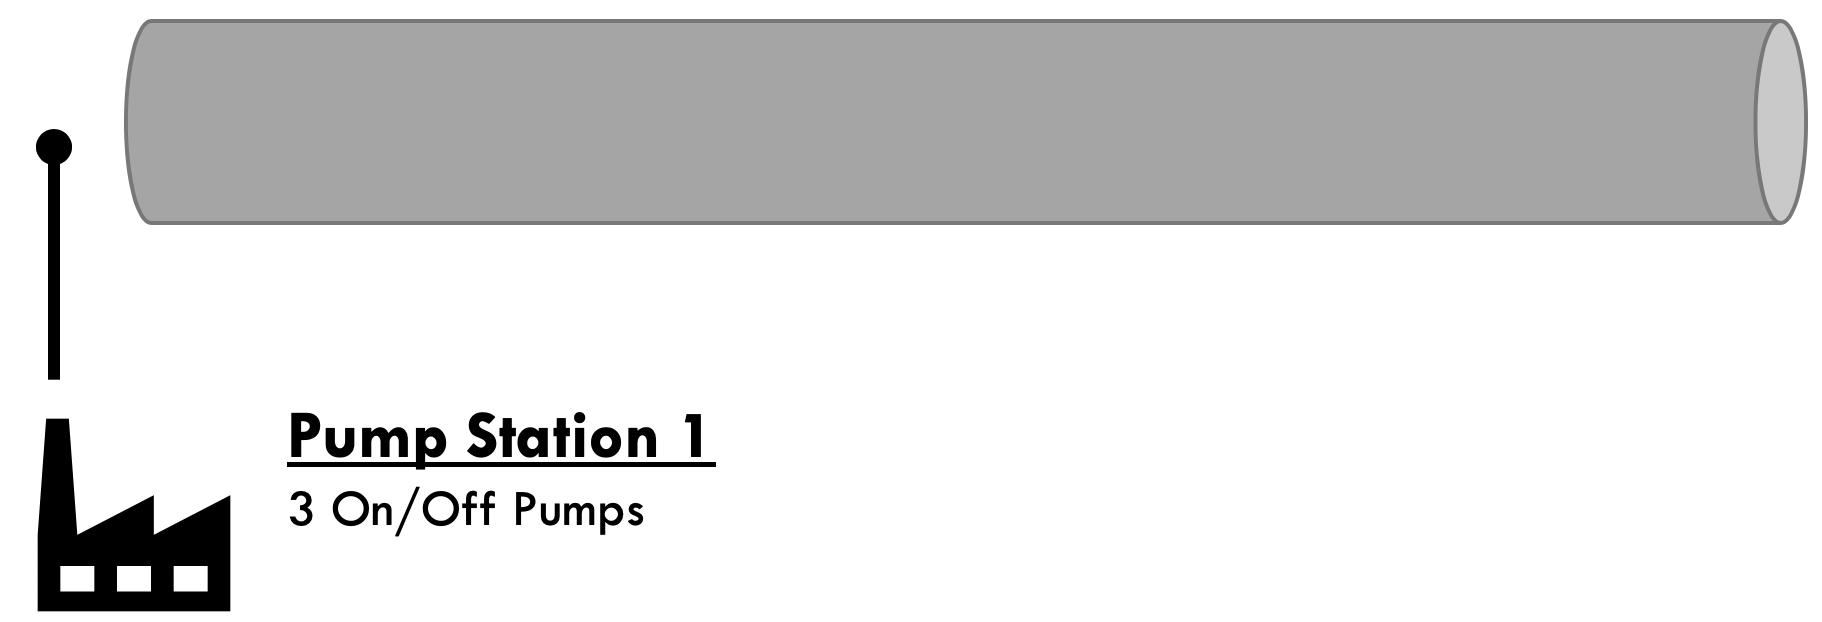
\includegraphics[scale=0.45]{images/08Line11.png}
    \caption{Schematic diagram of Line 11.}
    \label{fig:08Line11}
\end{figure}


\subsection{Line RM06A}
A schematic of line RM06A is shown in Figure \ref{fig:08RM06A}.  Line RM06A is a complex pipeline spanning 151 km and carries two products, a lighter sweet product and a heavier sour product. The two products are batched (i.e., rotate between sending each product) and each product is sent for approximately eight hours before switching to the other product. The American Petroleum Institute (API) gravity for the lighter and heavier products are roughly 40 and 20, respectively. For the rest of this chapter, the lighter and heavier product will be referred to as \textit{sweet crude} and \textit{sour crude}, respectively. The pipeline is typically operated between 1500 bbl/h to 3050 bbl/h. 

\begin{figure}[h]
    \centering
    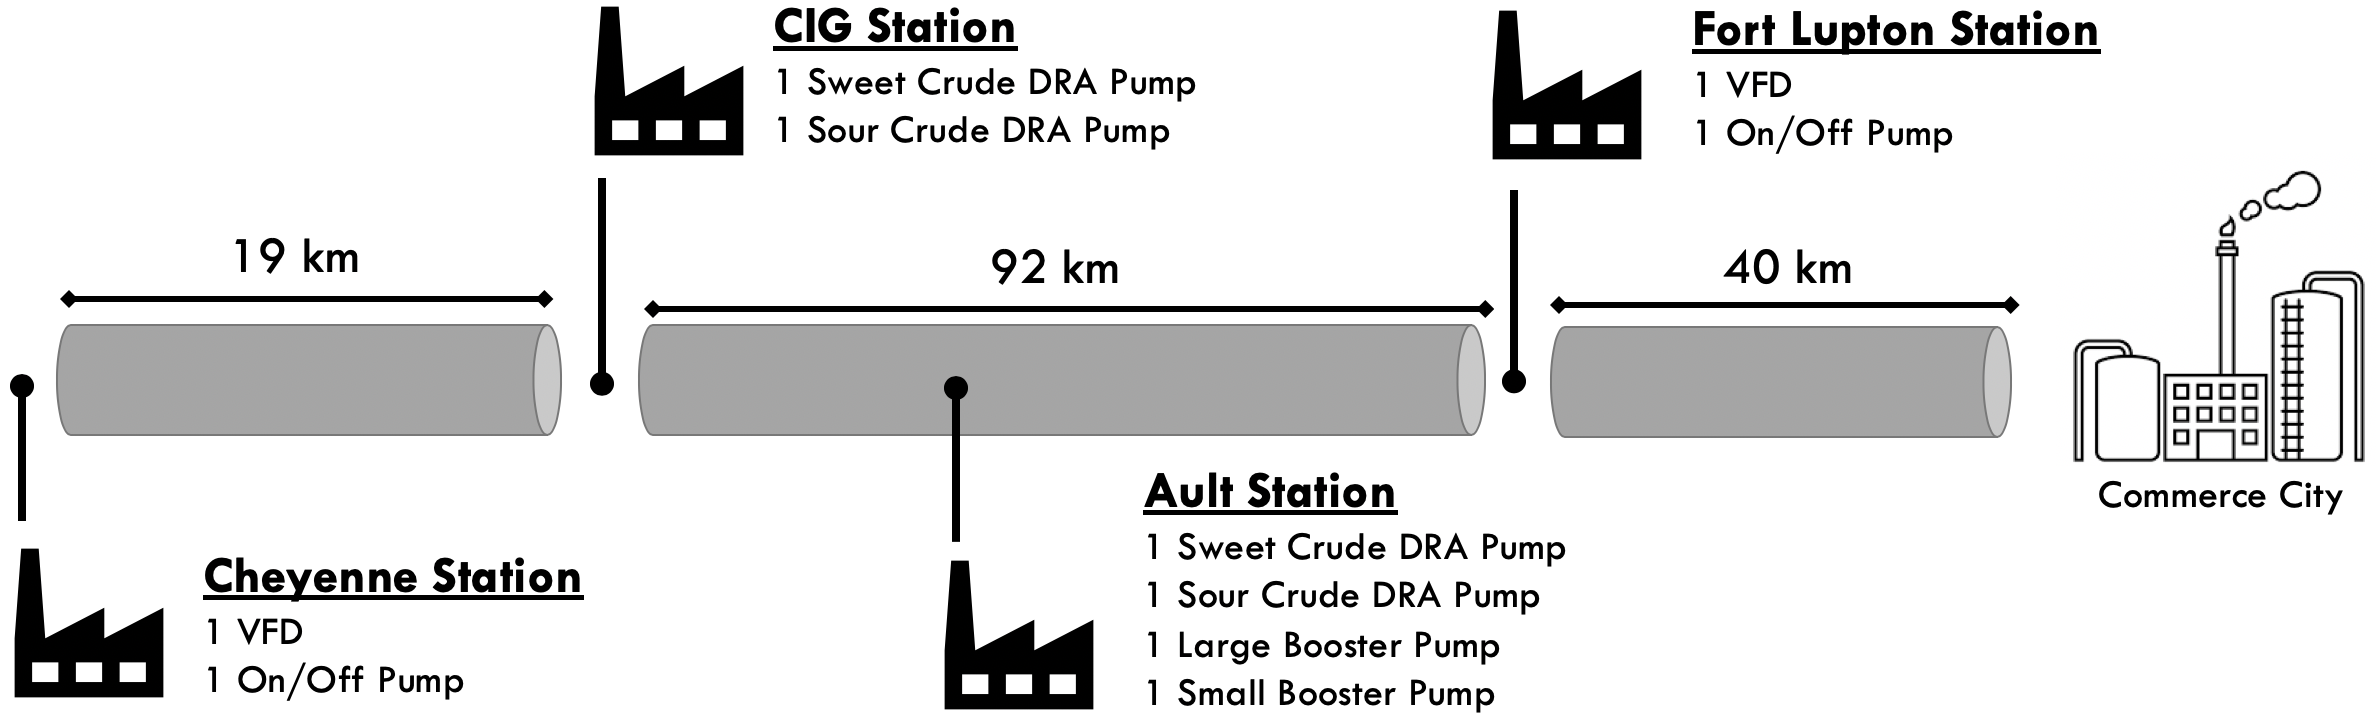
\includegraphics[scale=0.35]{images/08RM06A.png}
    \caption{Schematic diagram of Line RM06A.}
    \label{fig:08RM06A}
\end{figure}

Equipment wise, Line RM06A boasts eight pumps spread across four pump stations. Two pumps are variable frequency drives (VFD), while the rest are on/off pumps. Additionally, there are four drag reducing agent (DRA) injection pumps situated across the second and third pump stations. Each pump station contains a sour crude and sweet crude DRA pump. The sour and sweet crude uses different types of DRA.  The DRA is injected based on the product present at the pump station. 

\section{Anomaly Detection}
\subsection{Data Pre-processing}
\subsection{Data Set Creation}
\subsubsection{Generative Modelling}
\subsection{Model Identification}
\subsection{Conceptual Software Design}

\section{Real Time Optimization}
Modern control systems typically consists of three layers: real time optimization (RTO), supervisory control and regulatory control.  From the top, real time optimization is evaluated the least frequently, and performs a steady state optimization of the process.  The outputs of RTO are the ideal set points for all equipment given an operating objective.  Next, the supervisory control layer performs dynamic optimization to identify the most efficient input trajectory to achieve the set points from RTO. Supervisory control is evaluated faster than RTO, but slower than regulatory control. Model predictive control (MPC) and economic model predictive control (EMPC) are typical supervisory control frameworks. Finally, the regulatory controllers actuate physical equipment to achieve the input trajectory given by the supervisory control layer.  Common regulatory controllers are proportional-integral-derivative (PID) controllers.

The hierarchical structure of APC is shown in Figure \ref{fig:08APC}.

\begin{figure}[h]
    \centering
    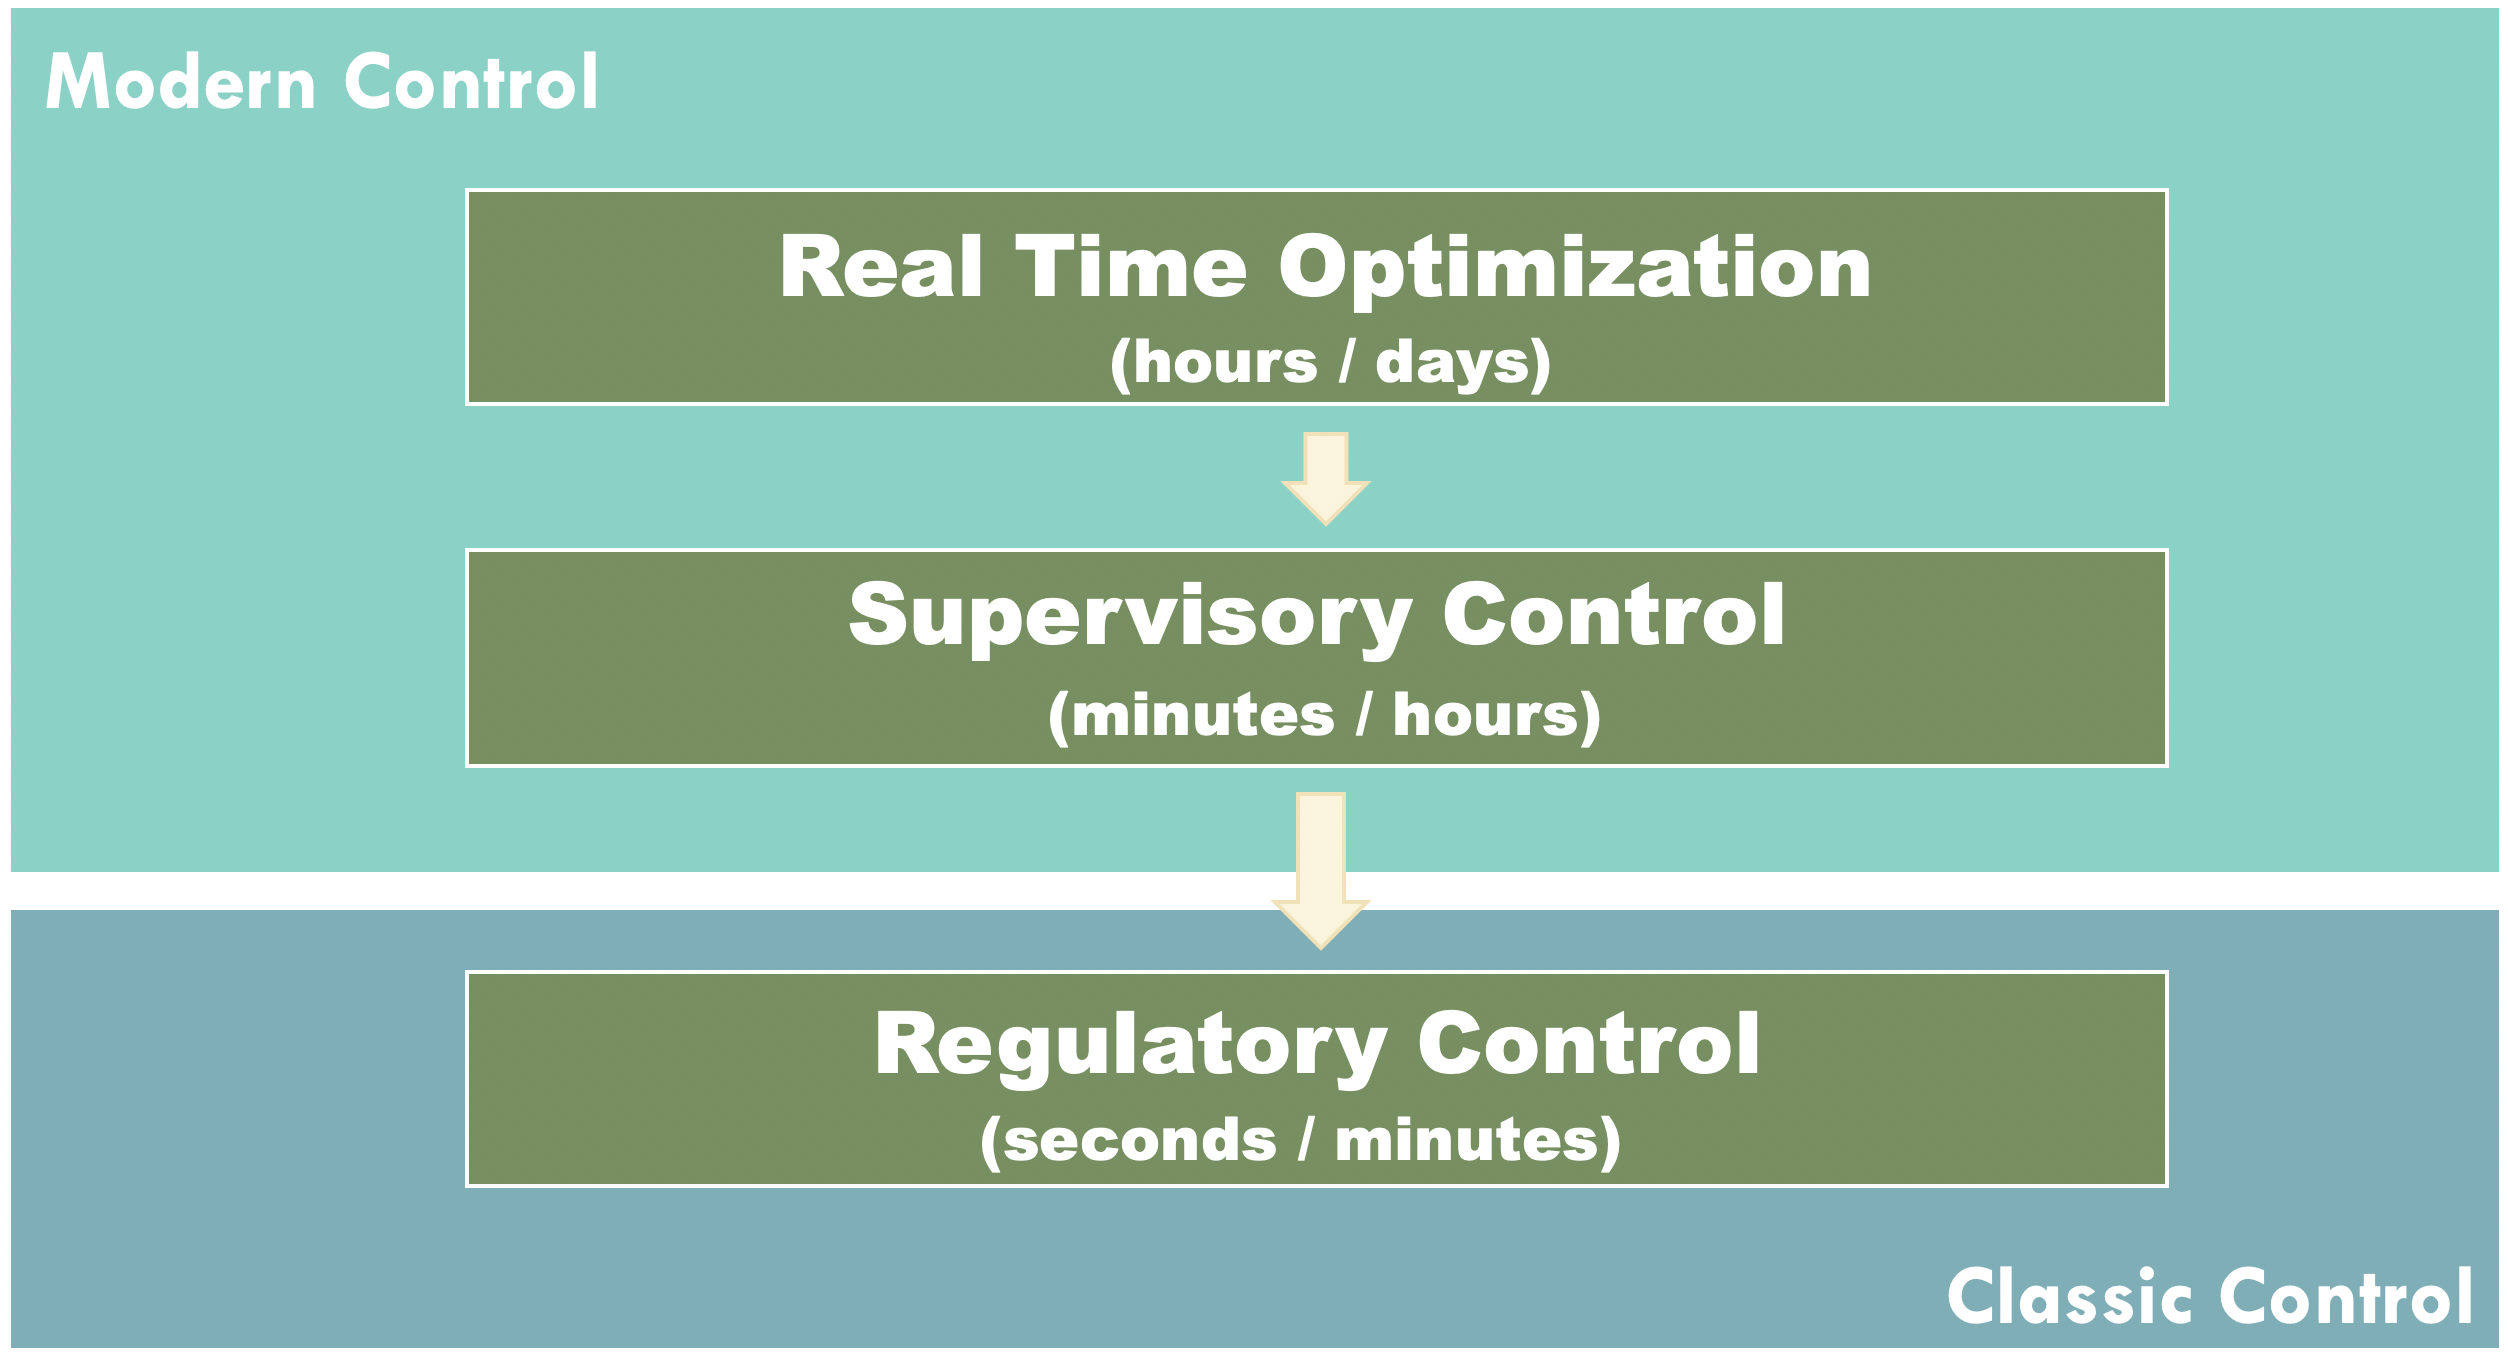
\includegraphics[scale=0.15]{images/08APC.png}
    \caption{Hierarchy of a typical control system.}
    \label{fig:08APC}
\end{figure}

\subsection{Problem Description}
Figure \ref{fig:08schedule} shows the communication framework of the pipeline operation. The goal of this pipeline is to meet the demands of the Commerce City refinery. To do so, a schedule with desired flow rates are sent to the operators from the scheduling team, and the operators are tasked to operate the pipeline at the given flow rate. Due to the complexity of this pipeline, different operators operate the pipeline differently depending on their own experience.  This difference introduces turbulence and unnecessary wear-and-tear onto the pipeline, increasing maintenance costs. Moreover, some operators are less experienced and operate the pipeline sub-optimally.

\begin{figure}[h]
    \centering
    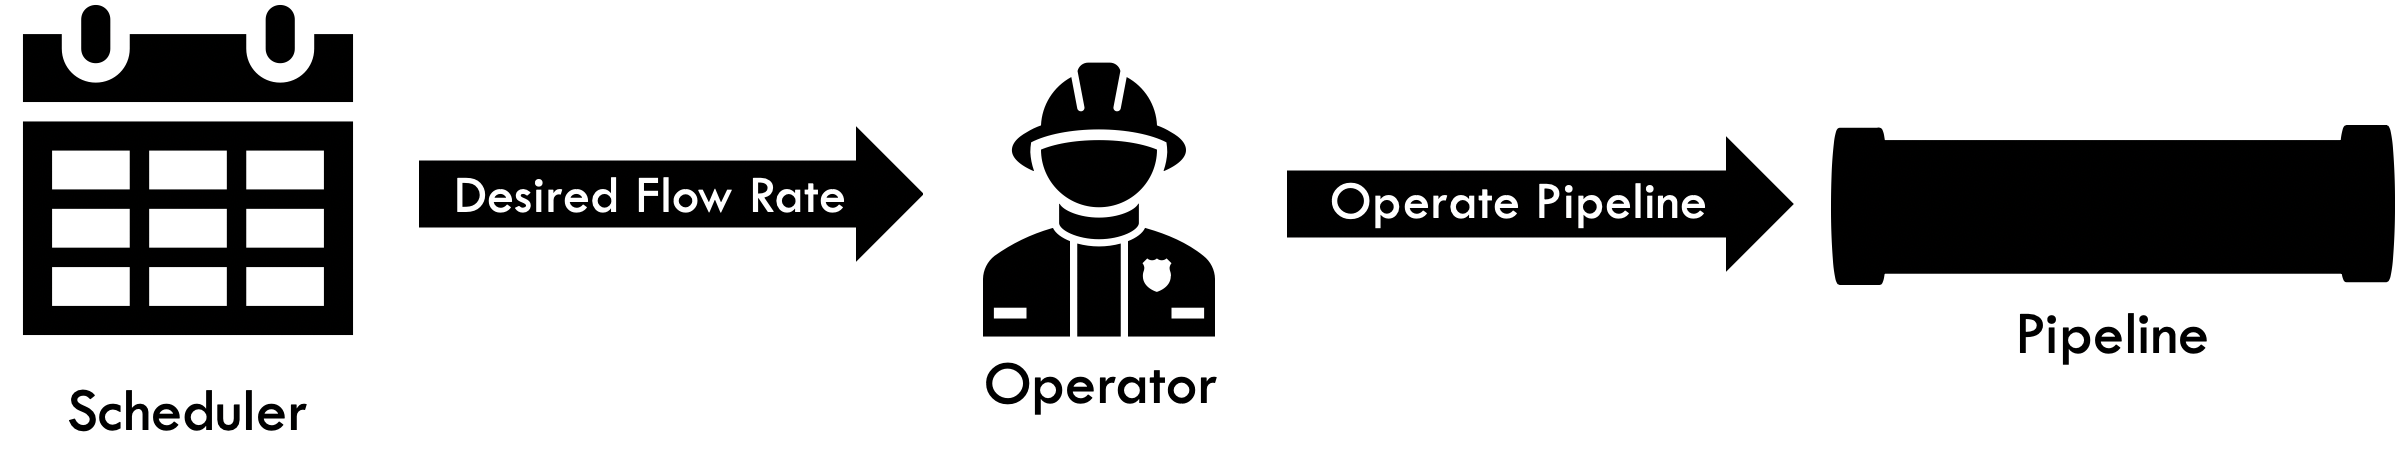
\includegraphics[scale=0.35]{images/08Schedule.png}
    \caption{Communication framework for operating line RM06A.}
    \label{fig:08schedule}
\end{figure}

To overcome this problem, machine learning was used to identify a model of the pipeline.  Then, a steady state optimization tool was built using mixed integer linear programming to give operators the \textbf{optimal} set-points for each equipment.  This system solves two problems: i) Introduces uniformity in operator behaviour for desired set-points. ii) Semi-automation of the pipeline, freeing up operators' time for other tasks.

The new communication framework for line RM06A is shown in Figure \ref{fig:08scheduleV2}.

\begin{figure}[h]
    \centering
    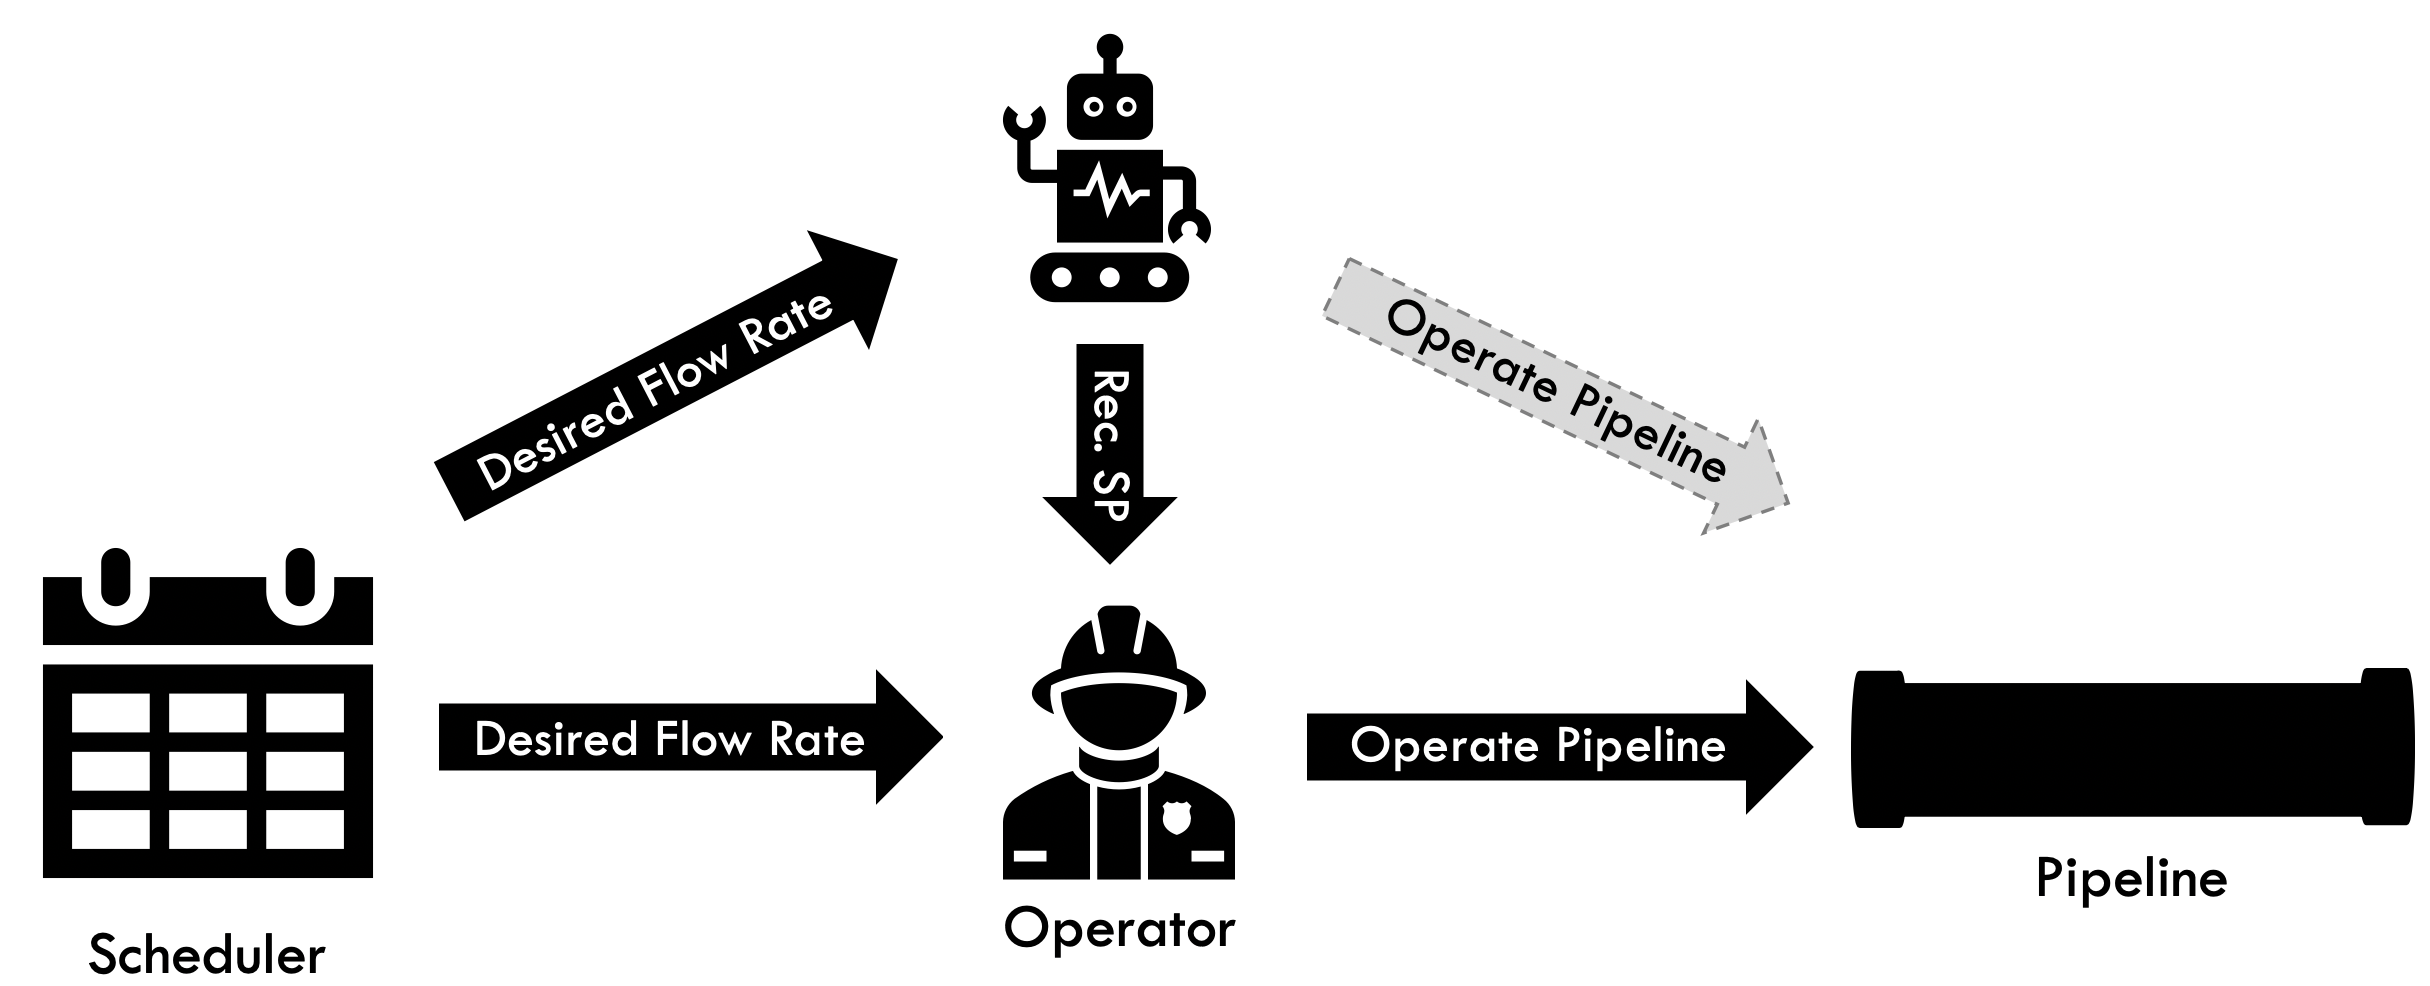
\includegraphics[scale=0.35]{images/08ScheduleV2.png}
    \caption{Proposed communication framework for operating line RM06A.}
    \label{fig:08scheduleV2}
\end{figure}

The rest of the section is organized as follows.  First, the data pre-processing step will be shown.  Then, the model identification phase will be introduced.  Following that, the optimization algorithm and all it's constraints for real-time optimization are presented.  Finally, the section is concluded with some conceptual software design regarding its implementation into a supervisory control and data acquisition (SCADA) system and the overall project impact will also be shown.

\subsection{Data Pre-processing}
Two data sets were initially provided by Suncor.  The details are shown in Table \ref{tab:08data}. Model identification and optimization evaluations were conducted for both datasets; however, the steps are very similar.  Because the 2019 algorithm will go into live production whereas the 2018 data was used primarily as a proof of concept, only the 2019 algorithm steps will be shown in detail.

\begin{table}[h]
    \centering
    {\setstretch{1.2}
    \begin{tabular}{ c | c }
        Date of Collection     &      Data Dimension      \\
        \hline
        June 2017 - June 2018  &    $525,601 \times 899$   \\
        Dec. 2018 - March 2019 &    $159,851 \times 738$   \\
    \end{tabular}}
    \caption{Suncor data details.}
    \label{tab:08data}
\end{table}

Data pre-processing can be broken down into three phases: Filtering by subject matter experts, automated data pre-processing, and manual data pre-processing.  An iterative procedure followed phase three where the subject matter experts worked alongside the machine learning scientists to give suggestions on which variables should be included/excluded in the final model.

\subsubsection{Filtering by Subject Matter Experts}
The first phase of data pre-processing was conducted by the subject matter experts at Suncor.  The original data set contained all data corresponding to the pipeline.  Variables such as alarm limits, fire detector status, monitor on/off status, etc., have low predictive power and were removed.  After this phase, the number of variables reduced from 738 to 124.  

The distribution of the remaining variables along the pipeline can be seen in Table \ref{tab:08Ph1Data}.

\begin{table}[h]
    \centering
    {\setstretch{1.2}
    \begin{tabular}{ c | c | c | c | c | c | c}
             &  Cheyenne & CIG & Ault & Fort Lupton & Comm. City & Other      \\
        \hline
        \# of Variables  &  24  &  21  &  21  &  33  &  22  &  3  \\
    \end{tabular}}
    \caption{Distribution of variables along line RM06A after phase 1 data pre-processing.}
    \label{tab:08Ph1Data}
\end{table}

\subsubsection{Automated Data Pre-processing}
Next, the data set was automatically filtered using the following methods:

\begin{itemize}
    \item \textbf{Missing data removal}: Remove \textit{rows} of data containing missing data.
    \item \textbf{Data imbalance analysis}: Remove boolean variables that contain 97\% or more of a single class.  Heavily imbalanced variables create model biases towards the majority class \cite{data_preprocessing}.
    \item \textbf{Collinear analysis}: Identify variables that are correlated over 90\%. Correlation, $r_{xy}$ is given in Equation \ref{eq:08correlation}. After corrlated variables are identified, one variable is kept while the rest are removed.  This is done to avoid redundant parameters \cite{data_preprocessing}.
    \begin{equation}
        r_{xy} = \frac{\sum(x_i - \bar{x})(y_i - \bar{y})}{\sqrt{\sum(x_i - \bar{x})^2\sum(y_i-\bar{y})^2}}
        \label{eq:08correlation}
    \end{equation}
    
\end{itemize}

After performing the above methods, the data set reduced from 124 to 65. The distribution of the new data set is shown in Table \ref{tab:08Ph2Data}.
\begin{table}[h]
    \centering
    {\setstretch{1.2}
    \begin{tabular}{ c | c | c | c | c | c | c}
             &  Cheyenne & CIG & Ault & Fort Lupton & Comm. City & Other      \\
        \hline
        \# of Variables  &  10  &  11  &  11  &  18  &  12  &  3  \\
    \end{tabular}}
    \caption{Distribution of variables along line RM06A after phase 2 data pre-processing.}
    \label{tab:08Ph2Data}
\end{table}

\subsubsection{Manual Data Pre-processing}
The data set is then manually pre-processed to remove or modify data from badly behaving sensors and irregular operating conditions.  In this phase, only the number of training examples are reduced.

For this pipeline, both sweet and sour crude are transported in a cyclical fashion due to the hydraulic dynamics of the pipeline. Otherwise, the sour crude is too heavy to be transported for sustainable periods. However, downstream demand for each product can disrupt this operating cycle.  From Figure \ref{fig:08API}, it can be seen that there were extended periods of time where only sweet or sour crude were being transported, and was caused by the lack of demand downstream.  Such scenarios deviate from normal operations and were removed from the data.

\begin{figure}[h]
     \centering
     \begin{subfigure}[b]{1.0\textwidth}
         \centering
         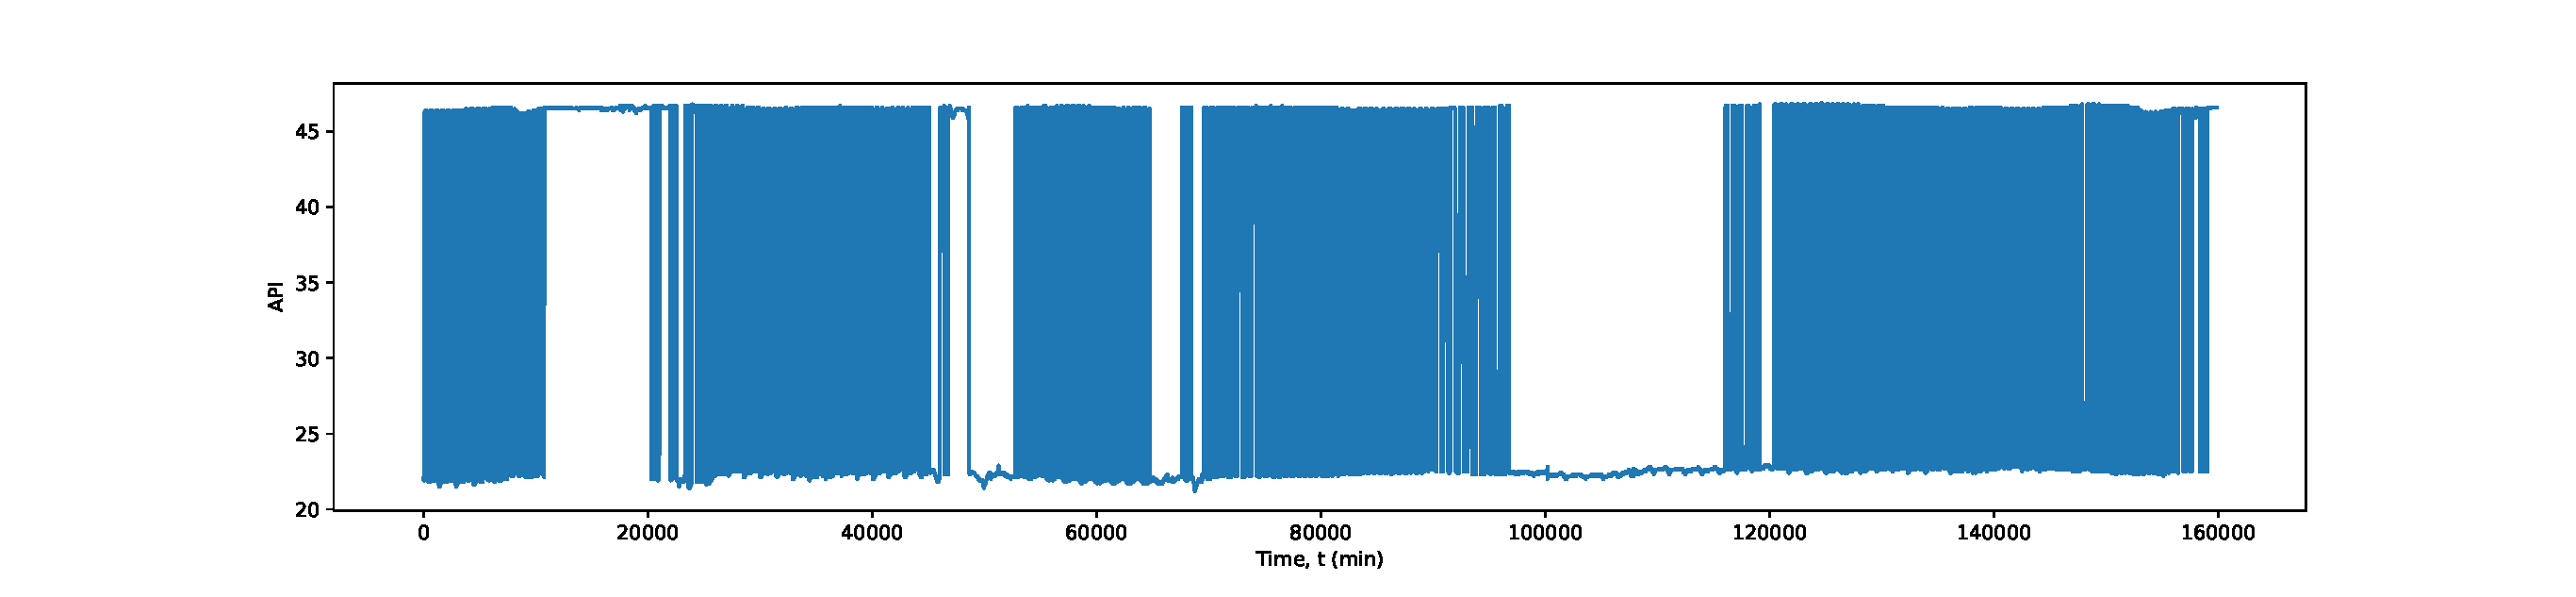
\includegraphics[width=\textwidth]{images/08NonFilteredDensity.eps}
         \caption{API data before abnormal condition removal.}
         \label{fig:08APIBefore}
     \end{subfigure}
     \hfill
     \begin{subfigure}[b]{1.0\textwidth}
         \centering
         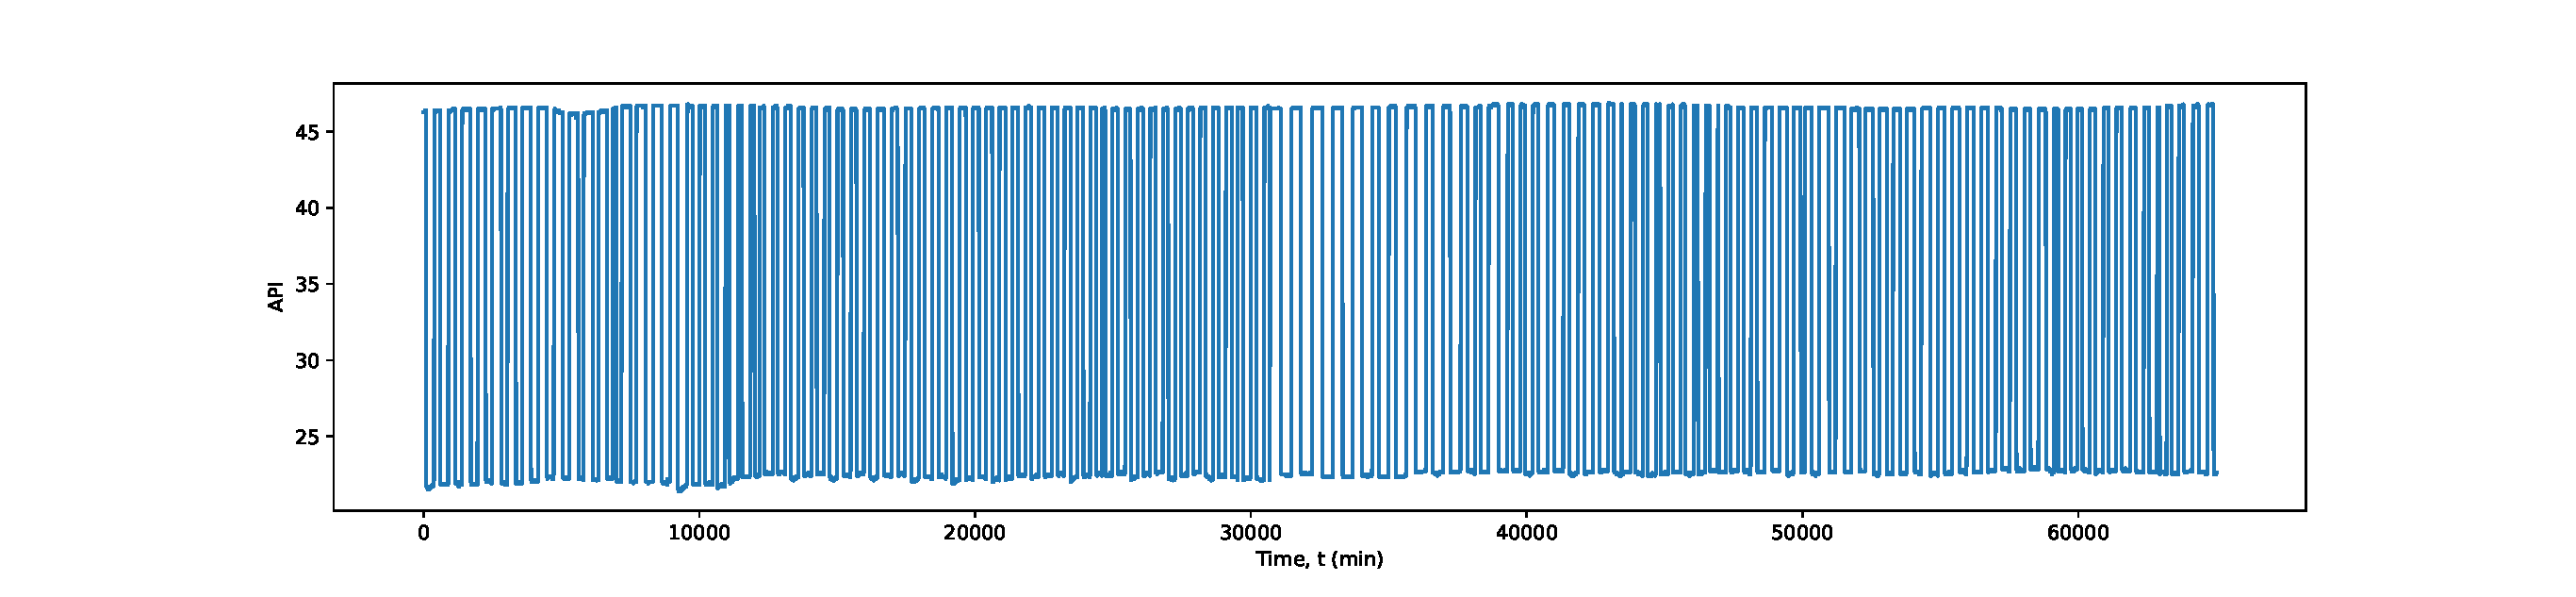
\includegraphics[width=\textwidth]{images/08FilteredDensity.eps}
         \caption{API data after abnormal condition removal.}
         \label{fig:08APIAfter}
     \end{subfigure}
        \caption{API data before and after removing abnormal operating conditions.}
        \label{fig:08API}
\end{figure}

Moreover, there is a time delay for the flow rate to react to a DRA set point change because the new DRA concentration must be transported throughout the line before its effect can be fully realized.  DRA is assumed to be catastrophically destroyed when passing through a pump; thus, DRA is only required to coat the pipeline between pump stations for its full effect to be exploited.  For CIG, it must coat the pipeline between CIG to Ault.  For Ault, the pipeline spanning between Ault and Fort Lupton must be coated.  Given the flow rate of the pipeline, it will take approximately ten hours to sufficiently coat the majority of the pipeline. Hence, data corresponding to transitional periods are removed. At times, transitional times may take longer; however, removing additional data will reduce the available data for model identification.  

Pre- and post-processed DRA parts per million (ppm) measurements are shown in Figure \ref{fig:08DRA}. DRA ppm is measured continuously for the control of the DRA injection pumps. However, the measurement is unreliable and corrupted with noise. Because DRA set points are rarely changed, an exponentially weighted moving average (EWMA) was applied to the DRA ppm readings for increased measurement reliability.  The EWMA formula and bias correction are given in Equations \ref{eq:08EWMA} and \ref{eq:08Bias_Correction}, respectively: 
\begin{equation}
    v_t = \beta v_{t - 1} + (1 - \beta) \theta_t, \; v_0 = 0
    \label{eq:08EWMA}
\end{equation}
\begin{equation}
    v_t \leftarrow \frac{v_t}{1 - \beta^t}, \forall v \in V
    \label{eq:08Bias_Correction}
\end{equation}
where $v_{t}$ is the exponentially weighted value at time $t$.  $\beta$ is the exponentially weighing factor.  Larger $\beta$ results in smoother results.  $\theta_t$ is the original value at time $t$. $V$ is a vector representing the exponentially weighted values before bias correction.

The objective of the machine learning model was to predict the flow rate at Commerce City.  However, there is a natural time delay between the time an equipment status changed and the corresponding impact on downstream flow rate.  Because the pipeline is fully loaded and the product is incompressible, pressure changes upstream will be propagated downstream at close to the speed of sound \cite{fluid_mechanics}.  Table \ref{tab:08TimeToCC} shows the time required for pressure to propagate down the pipeline starting from each pump station.  The pump data for each pump station was shifted accordingly to account for this time delay.  
\begin{table}[h]
    \centering
    {\setstretch{1.2}
    \begin{tabular}{ p{6cm} | c | c | c | c}
             &  Cheyenne & CIG & Ault & Fort Lupton \\
        \hline
        Time to Commerce City at speed of sound in liquids (1480 m/s) \cite{fluid_mechanics}
        &  1.7 min  &  1.5 min  &  1.0 min  &  0.45 min  \\
    \end{tabular}}
    \caption{Time required for pressure changes at each pump station to be realized at Commerce City.}
    \label{tab:08TimeToCC}
\end{table}
\begin{figure}
     \centering
     \begin{subfigure}[b]{0.9\textwidth}
         \centering
         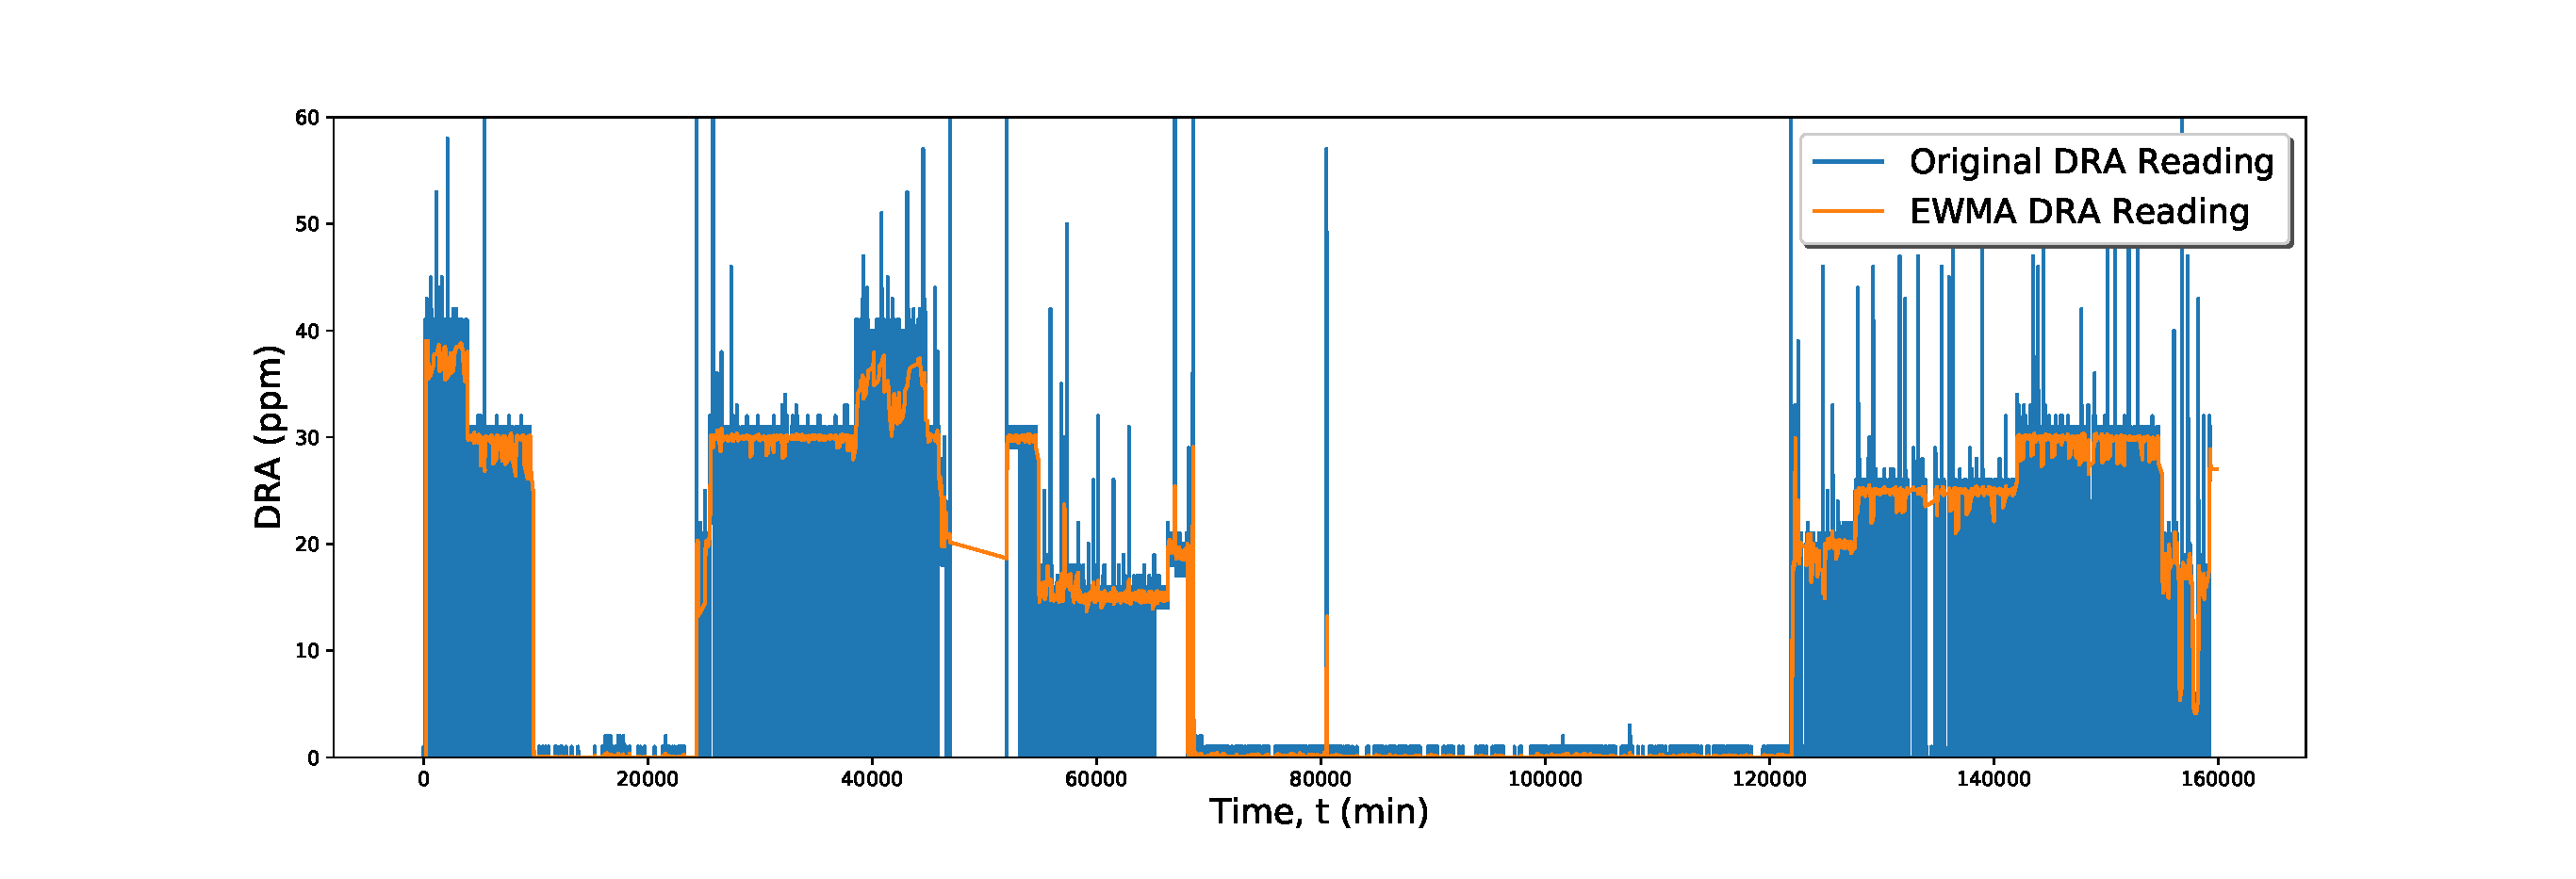
\includegraphics[width=\textwidth]{images/08CIGSour.eps}
         \caption{CIG sour DRA sensor reading.}
         \label{fig:08CIGSour}
     \end{subfigure}
     \begin{subfigure}[b]{0.9\textwidth}
         \centering
         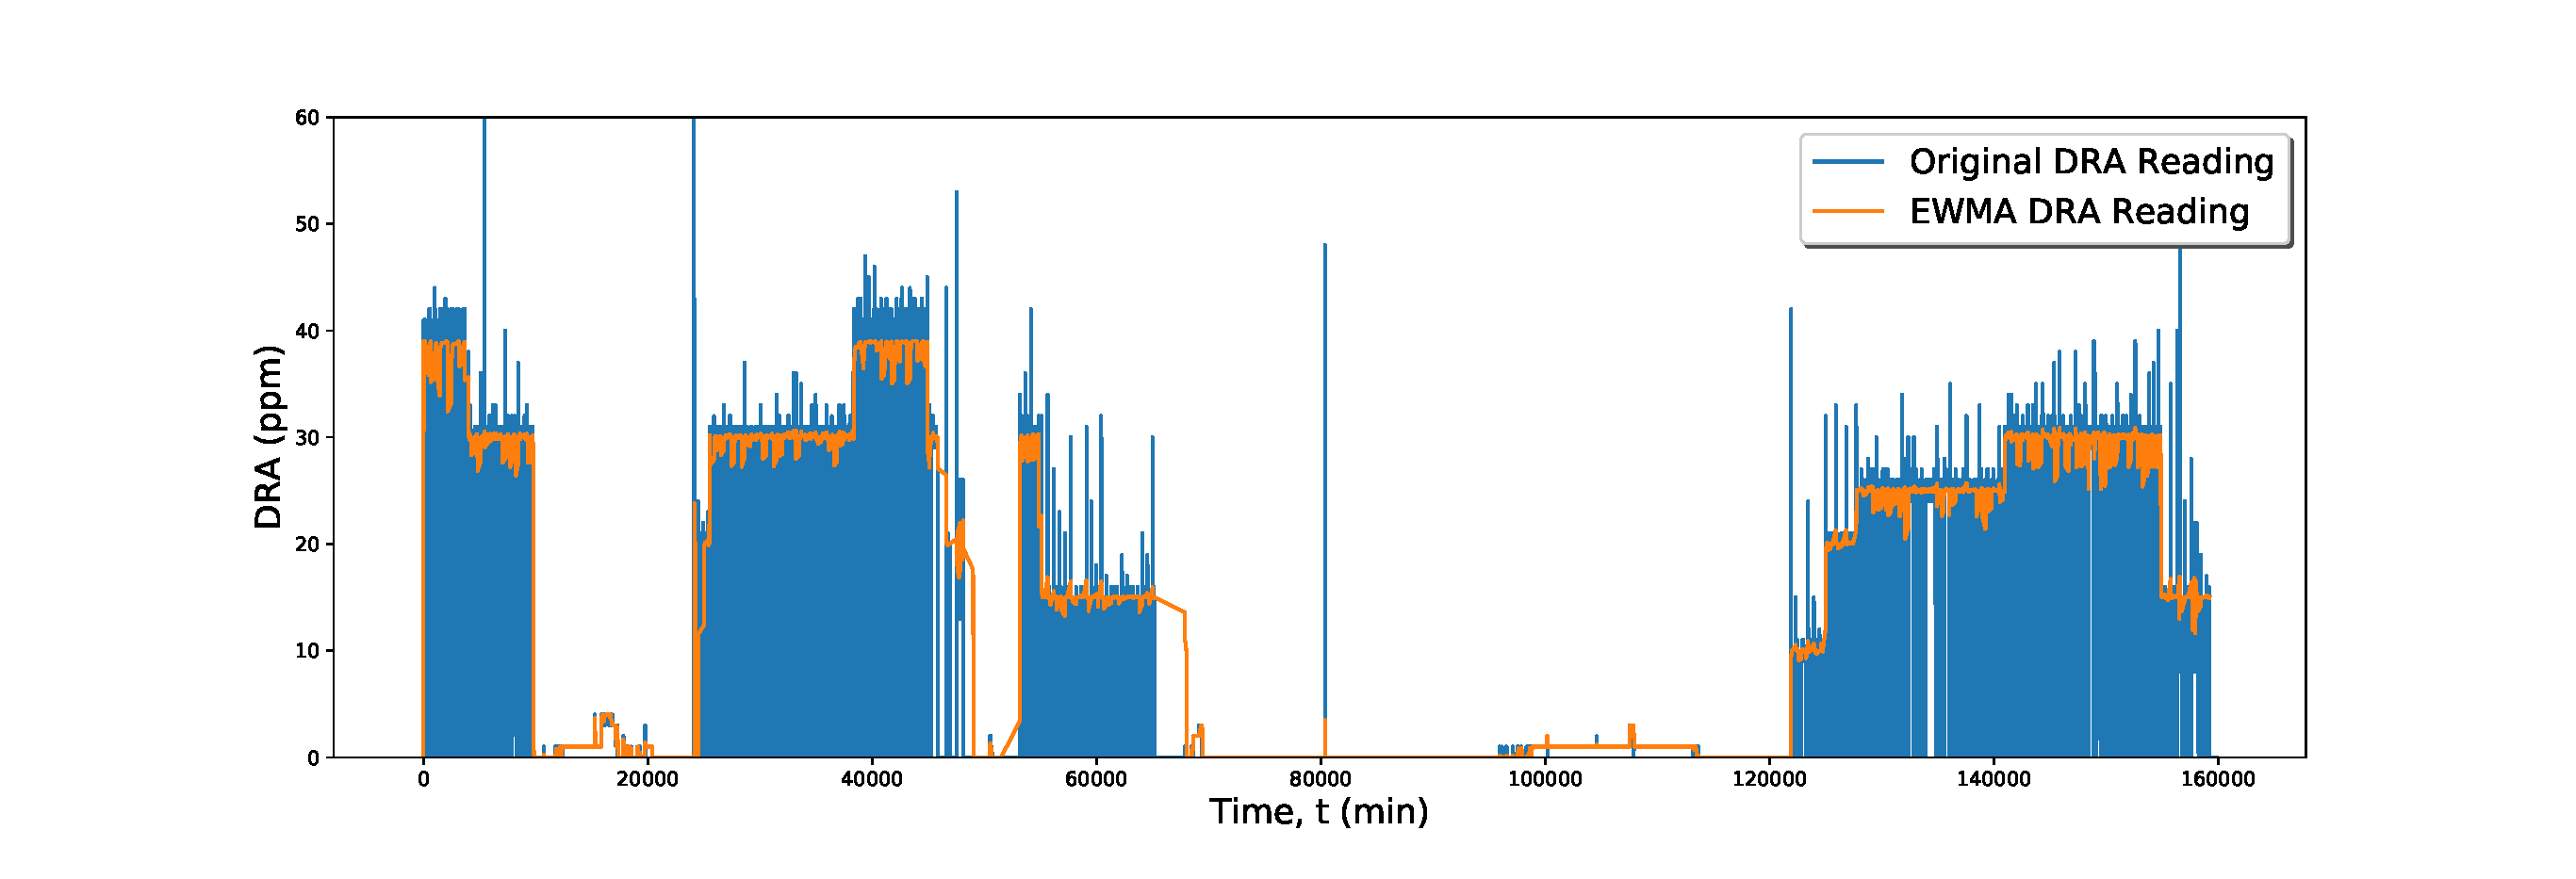
\includegraphics[width=\textwidth]{images/08CIGSweet.eps}
         \caption{CIG sweet DRA sensor reading.}
         \label{fig:08CIGSweet}
     \end{subfigure}
     \begin{subfigure}[b]{0.9\textwidth}
         \centering
         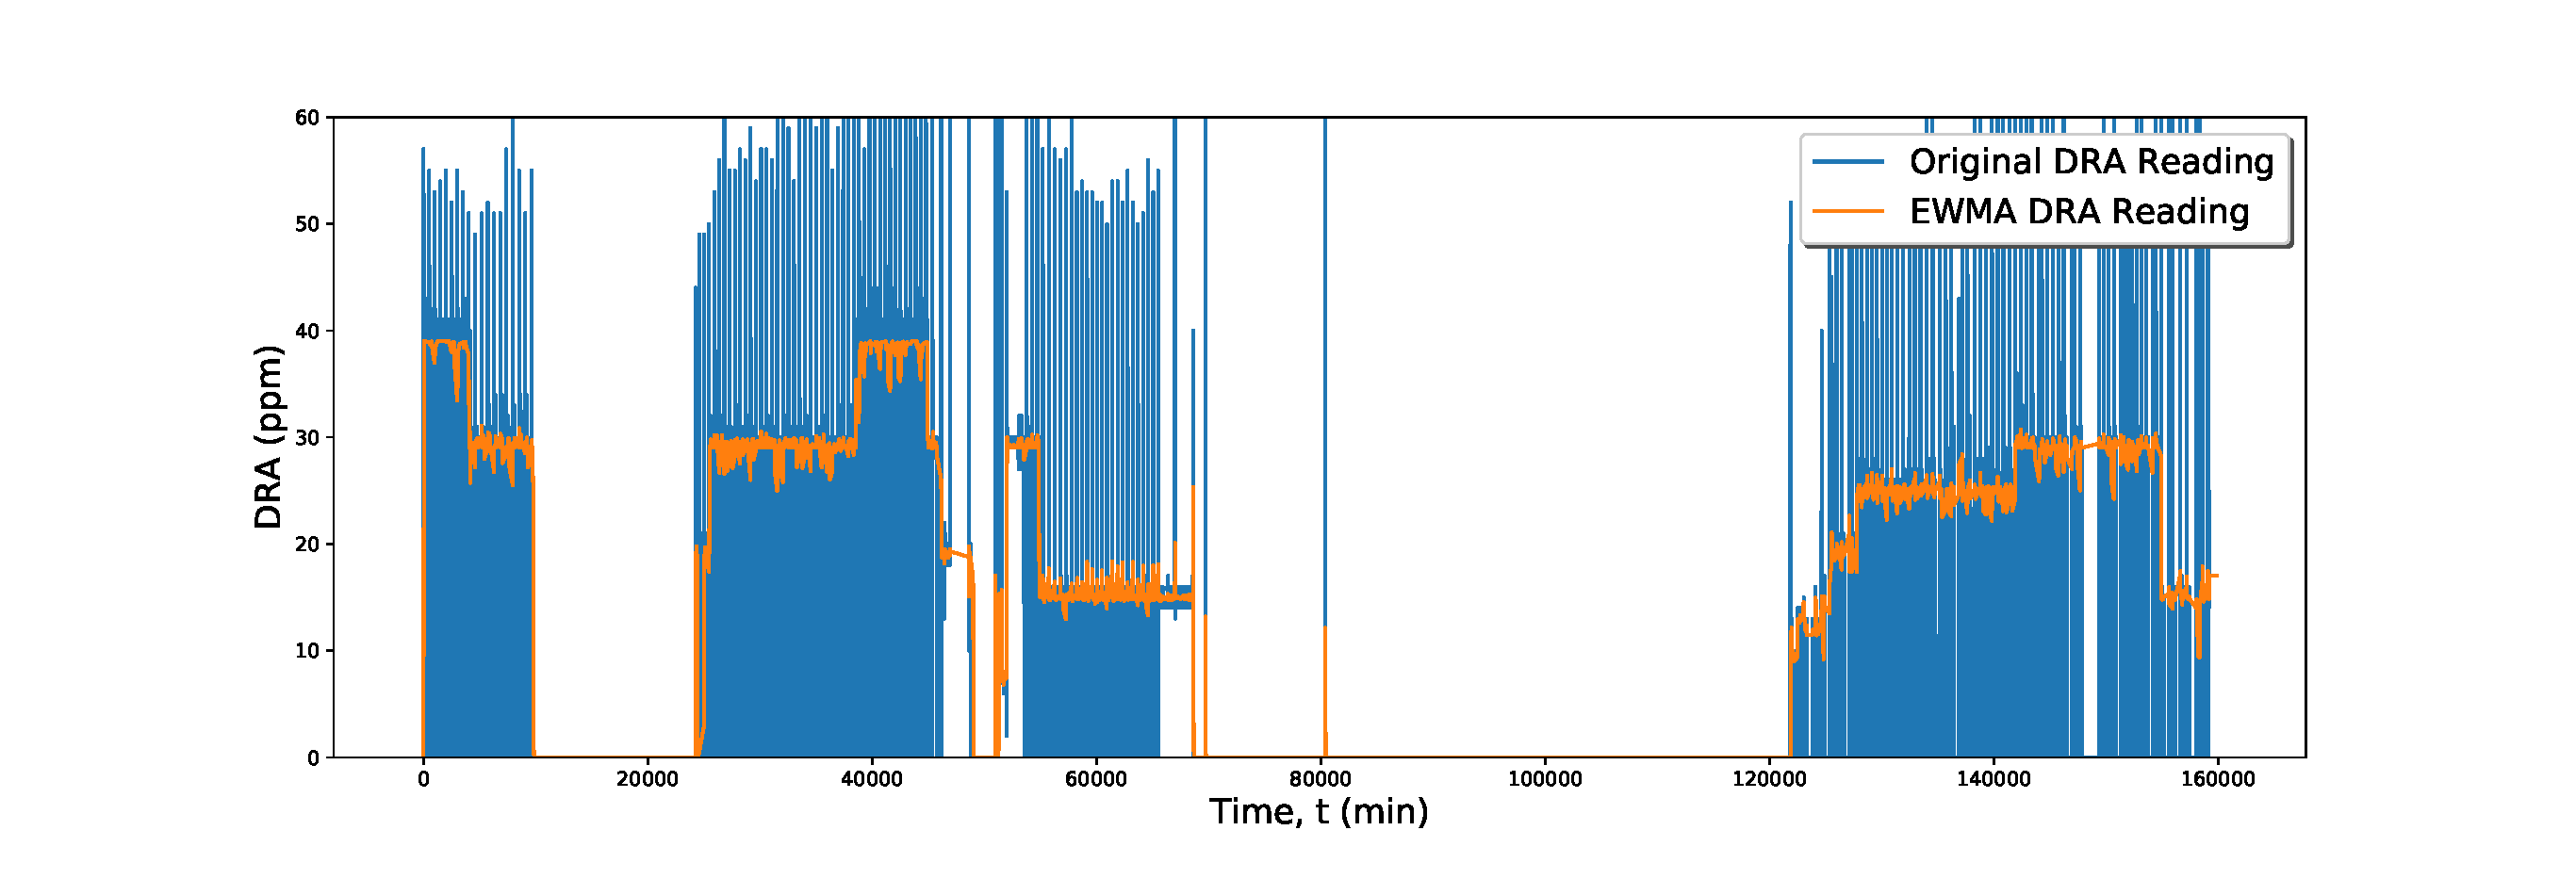
\includegraphics[width=\textwidth]{images/08AultSour.eps}
         \caption{Ault sour DRA sensor reading.}
         \label{fig:08AultSour}
     \end{subfigure}
     \begin{subfigure}[b]{0.9\textwidth}
         \centering
         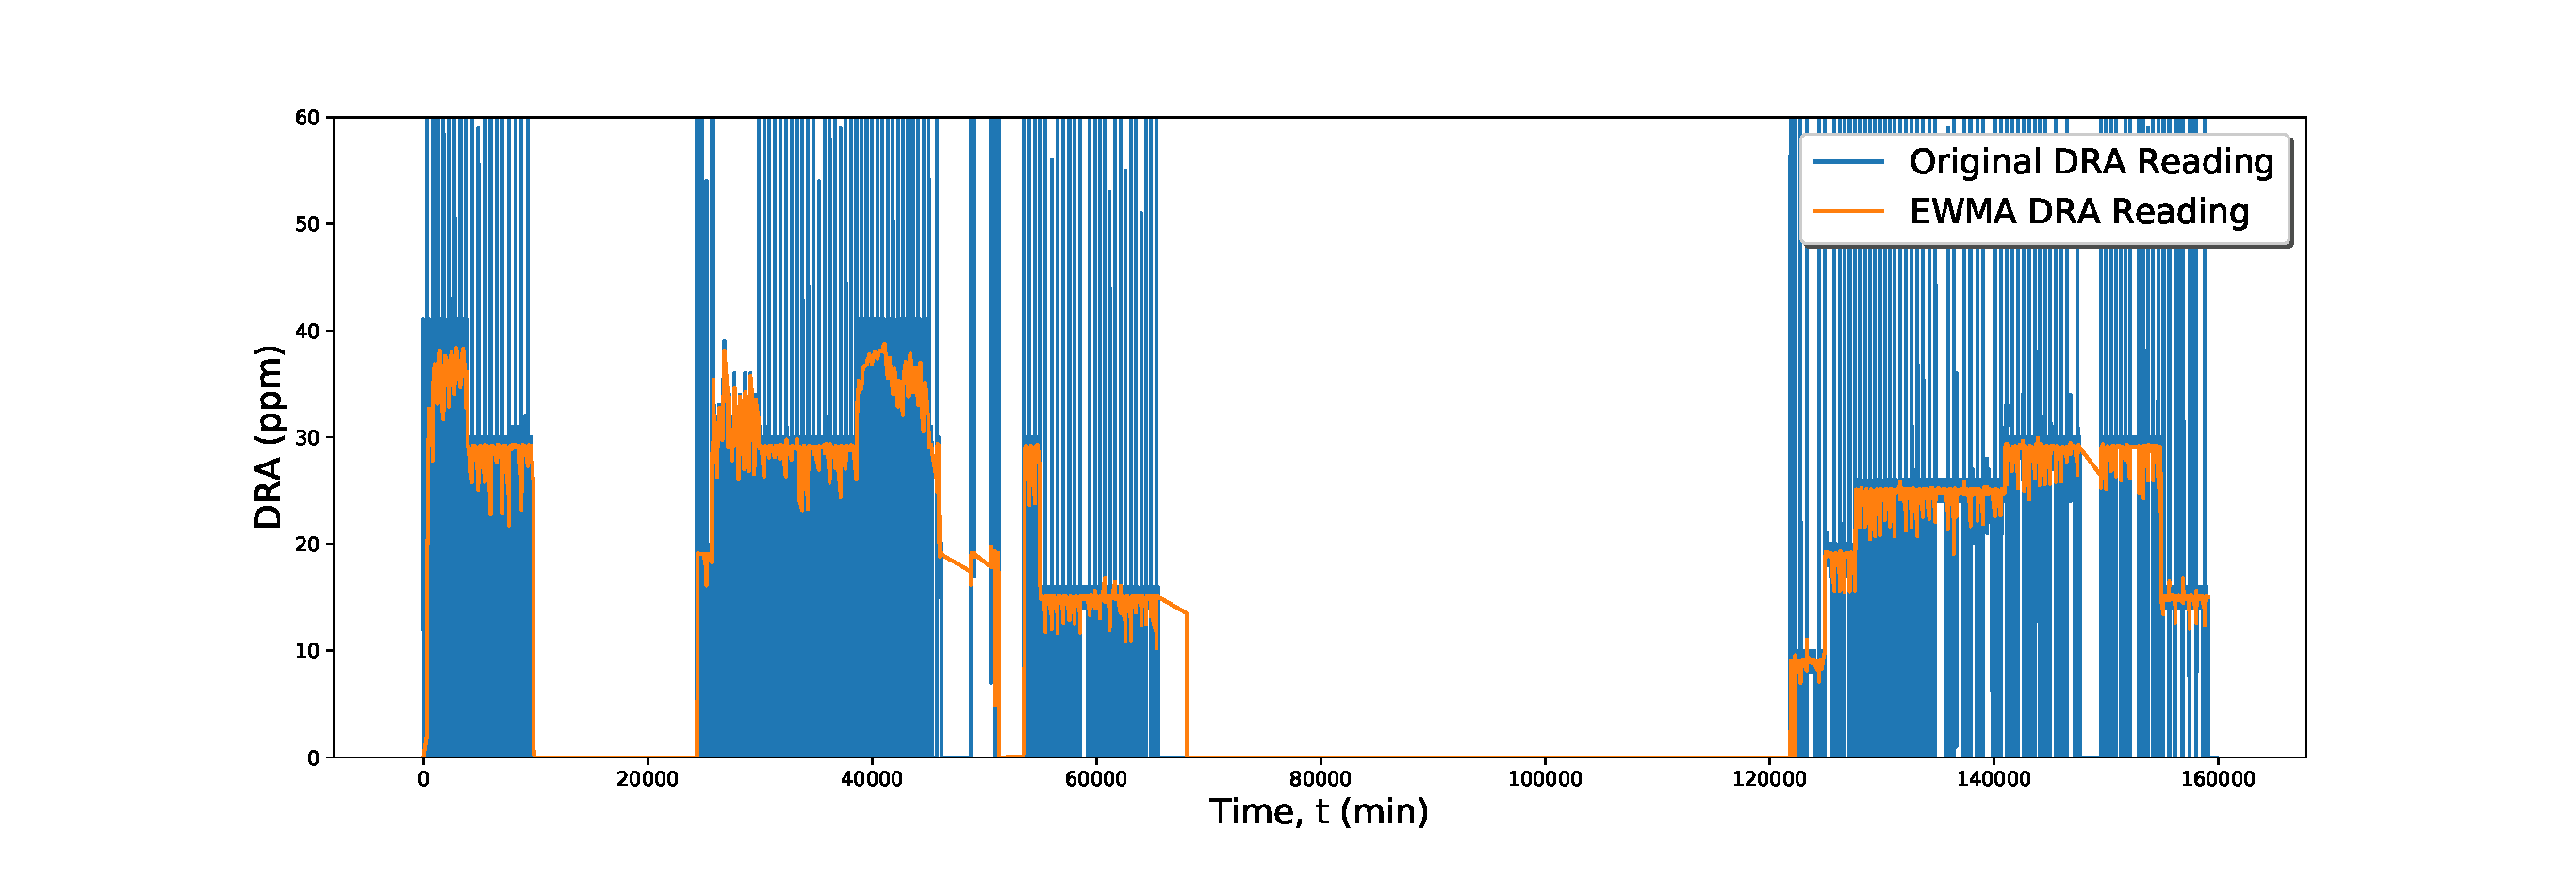
\includegraphics[width=\textwidth]{images/08AultSweet.eps}
         \caption{CIG sweet DRA sensor reading.}
         \label{fig:08AultSweet}
     \end{subfigure}
        \caption{Pre- and post-processed DRA sensor readings.}
        \label{fig:08DRA}
\end{figure}

A comprehensive list of the manual data pre-processing procedures is as follows:
\begin{enumerate}
    \item Shift data to accommodate the time delay at Commerce City.
    \item Smooth DRA data using exponentially weighted moving average given in Equation \ref{eq:08EWMA}.  
    \item Remove first 10 hours data corresponding to DRA set point changes.
    \item Remove data points where flow is under 800 bbl/hr.
    \item Remove data when only sweet or sour crude was sent through the pipeline.
\end{enumerate}

The final data set contained 65 variables and 97,470 data points.

\subsection{Model Identification}
\subsubsection{Feature Selection}
For each pump station, there was a variety of sensors measuring the same process variables.  For example, VFD pumps have four readings each: On/off status, RPM, HZ, and current. Many variables relating to one equipment is redundant; thus, only one variable was selected when redundancy existed. Additionally, some sensors were behaving abnormally.

In normal operations, the density fluctuates between 10 - 50 API, depending on the type of crude present in the pipeline.  After analysis, the Fort Lupton densitometer was behaving abnormally compared to other densitometer and is shown in Figure \ref{fig:08Density}.  After confirming with Suncor that the densitometer was behaving abnormally, the variable was removed.  
\begin{figure}[h]
     \centering
     \begin{subfigure}[b]{0.48\textwidth}
         \centering
         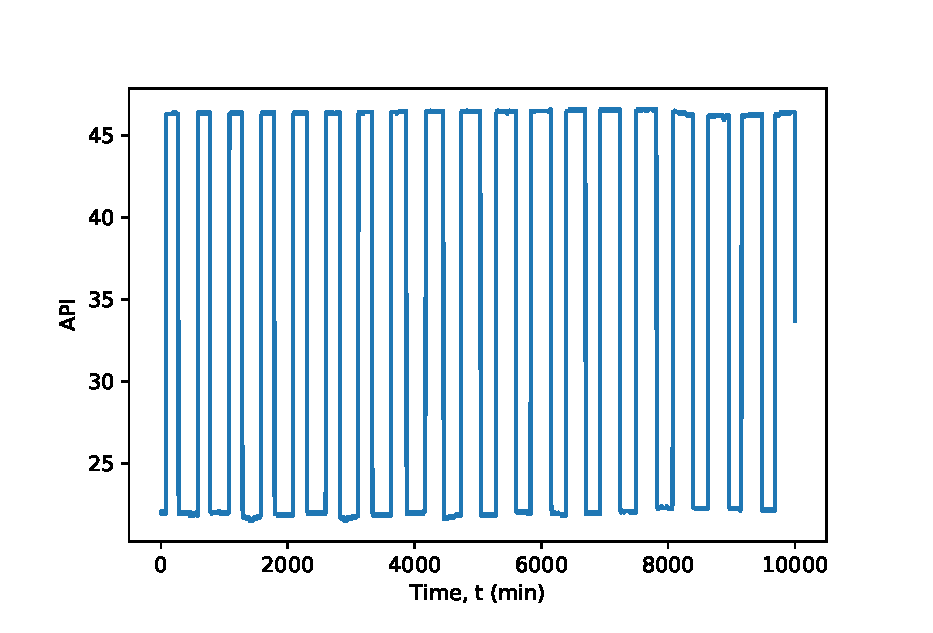
\includegraphics[width=\textwidth]{images/08CheyDensity.eps}
         \caption{Cheyenne API data for 10,000 mins.}
         \label{fig:08GoodDensity}
     \end{subfigure}
     \hfill
     \begin{subfigure}[b]{0.48\textwidth}
         \centering
         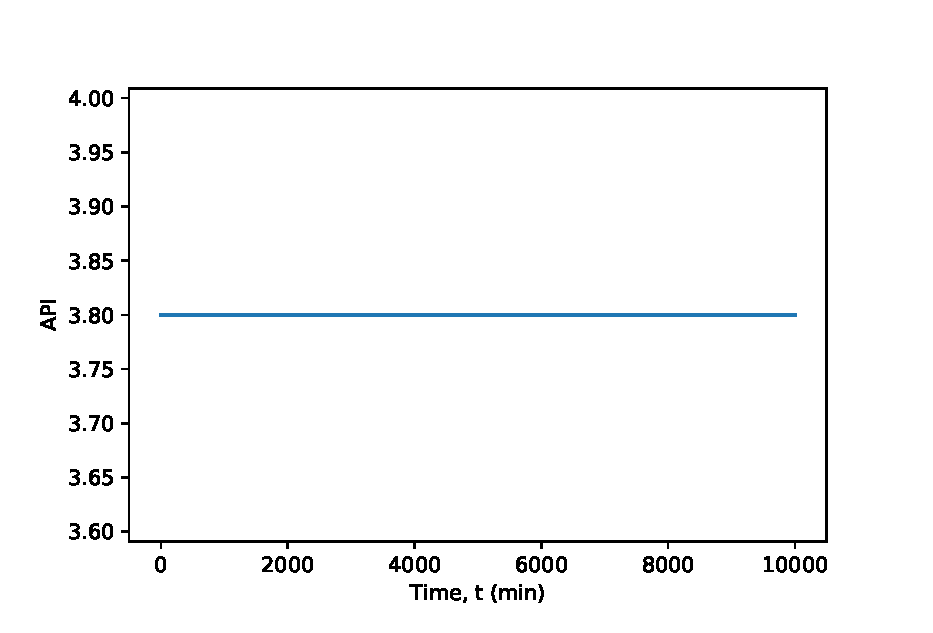
\includegraphics[width=\textwidth]{images/08FLDensity.eps}
         \caption{Fort Lupton API data for 10,000 mins.}
         \label{fig:08BadDensity}
     \end{subfigure}
        \caption{Comparison of normal and abnormal density readings.}
        \label{fig:08Density}
\end{figure}

Table \ref{tab:08featselect} shows the features selected for each pump station. The predicted variable was the flow rate (bbl/h) at Commerce City.
\begin{table}[h]
    \centering
    {\tiny
    {\setstretch{1.2}
    \begin{tabular}{ c | c | c | c | c}
        Cheyenne                       & CIG                      & Ault                        & Fort Lupton                    & Commerce City \\
        \hline
        $u_5$: Boos. Pump Status       &  $u_1$: Sweet DRA (ppm)  &  $u_3$: Sweet DRA (ppm)     &  $u_{8}$: Boos. Pump Status   &  $x_{8}$: Inlet Temp. (°C) \\
        
        $u_9$: VFD Current (Amp)       &  $u_2$: Sour DRA (ppm)   &  $u_4$: Sour DRA (ppm)      & $u_{10}$: VFD Current (Amp)      & \\
        
        $x_{4}$: Inlet Temp. (°C)     &  $x_{5}$: Inlet Temp. (°C) &  $u_6$: Small Pump Status &  $x_{7}$: Inlet Temp. (°C)  & \\
        
        $x_{1}$: API                   &  $x_{2}$: API          &  $u_7$: Large Pump Status   &             
        & \\
        
                                       &                          &  $x_{6}$: Inlet Temp. (°C)  &             
        & \\
        
                                       &                          &  $x_{3}$: API               &       
        & \\
        
    \end{tabular}}}
    \caption{Features selected for machine learning models.}
    \label{tab:08featselect}
\end{table}

\subsubsection{Feature Scaling}
Figure \ref{fig:08featscale} shows the contour of a normalized and non-normalized cost function. It can be seen that the optimization of a non-normalized cost function can be significantly hindered depending on where the optimization is initialized.

\begin{figure}[h]
    \centering
    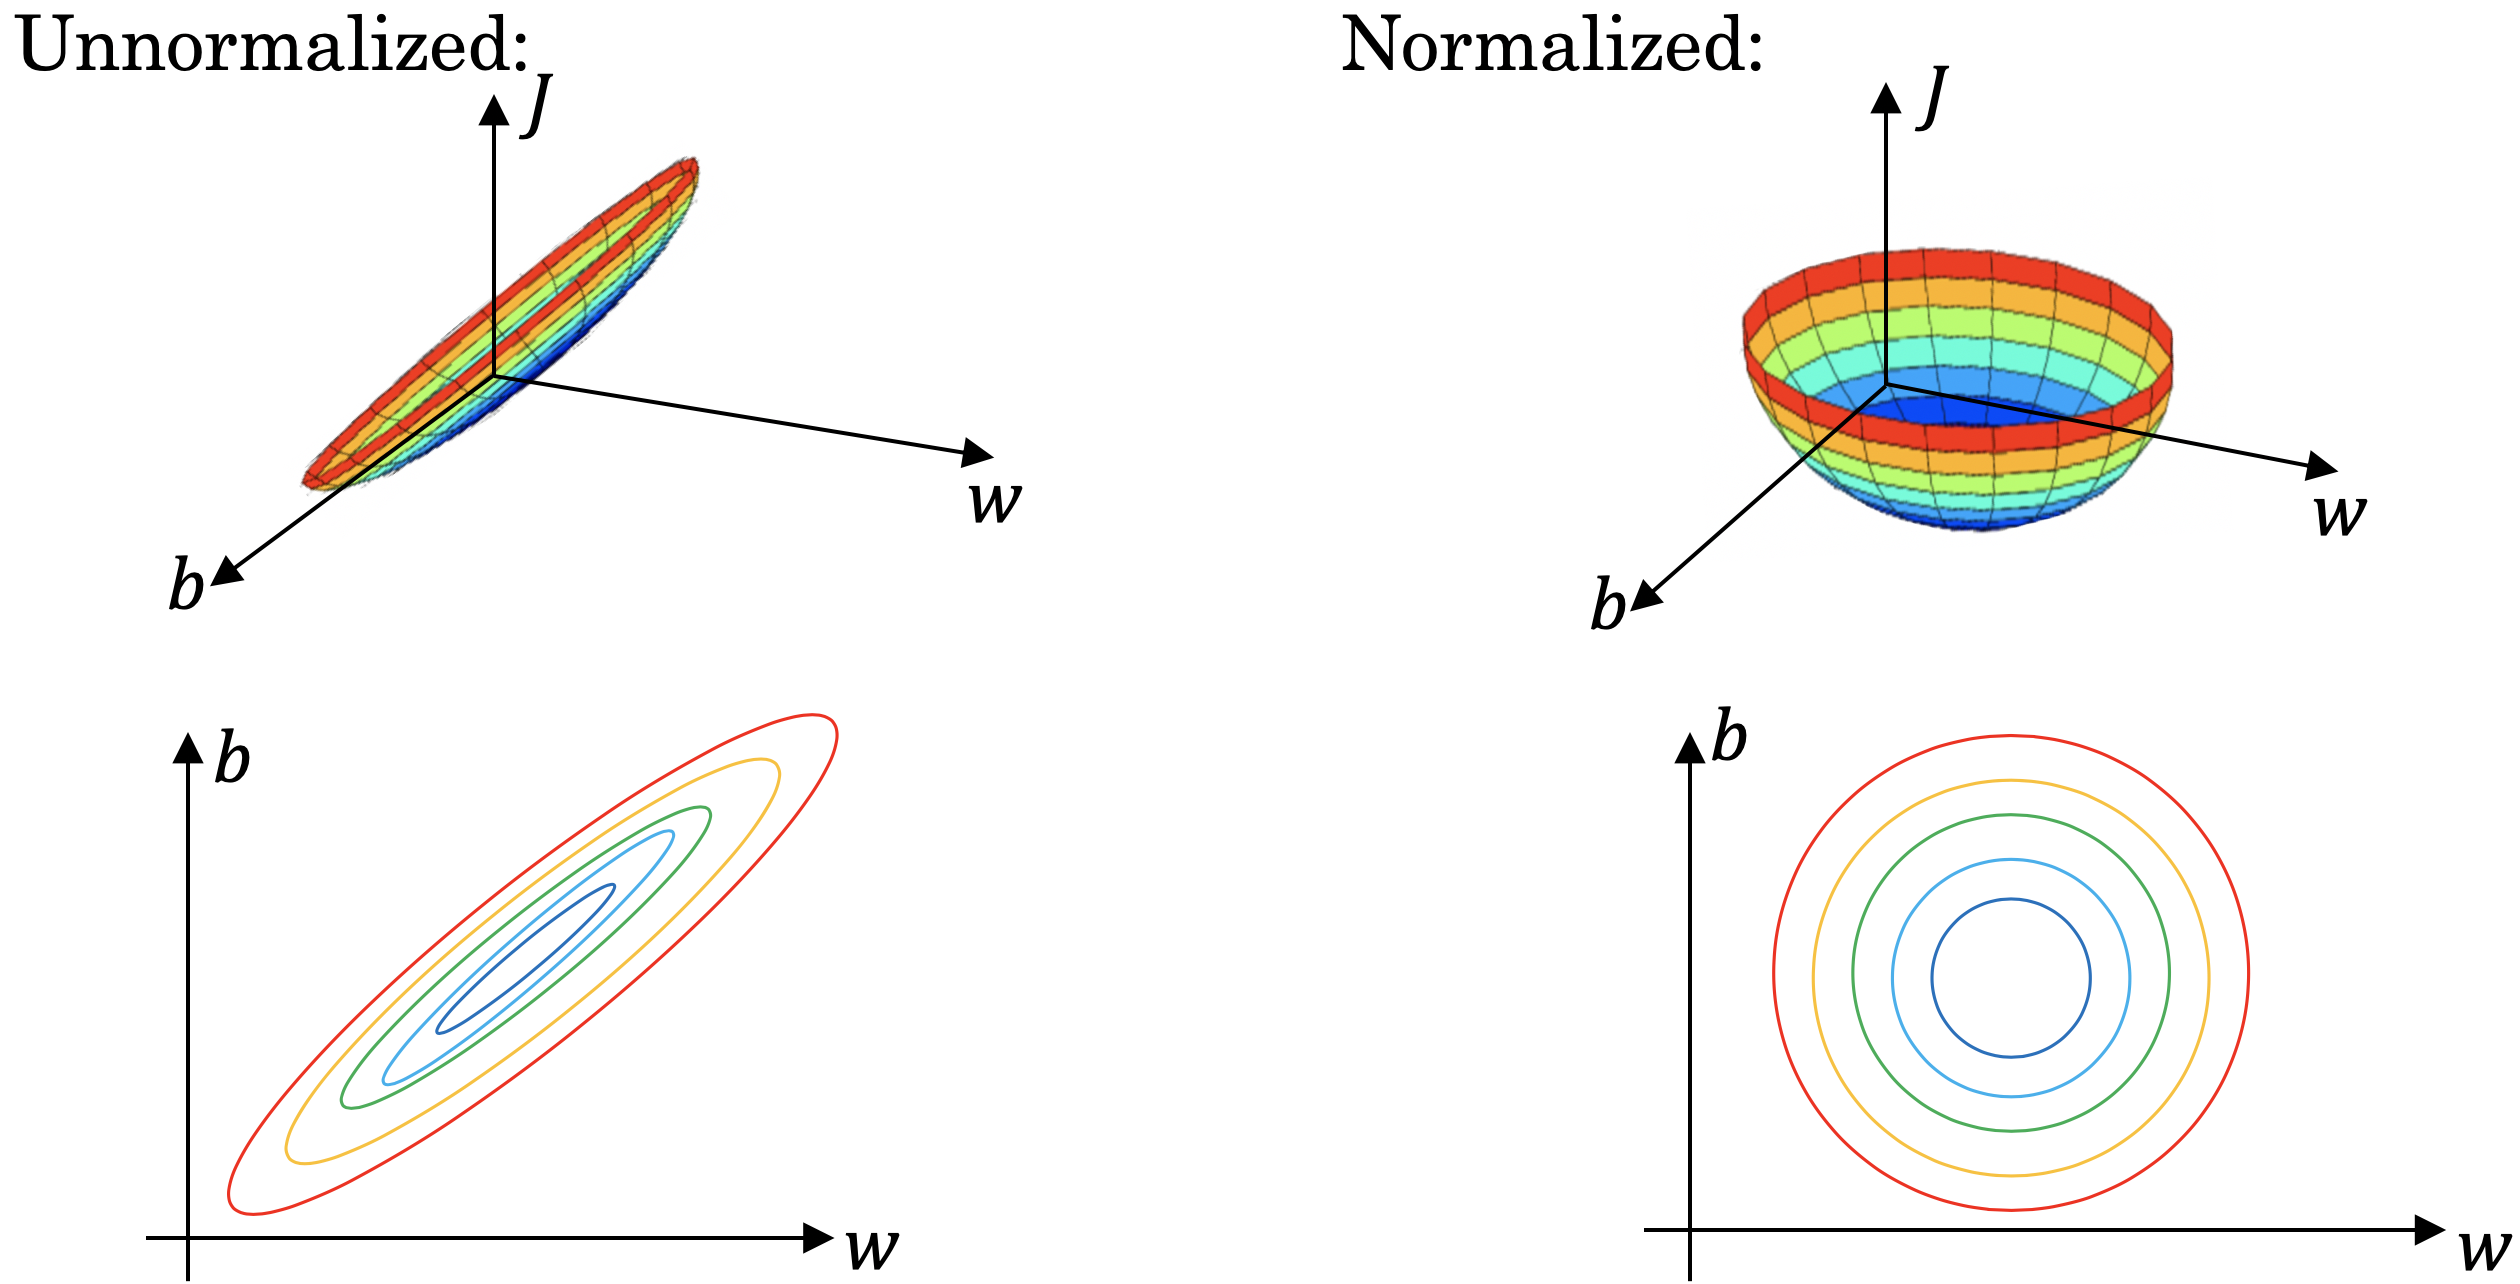
\includegraphics[width=.8\textwidth]{images/08featscale.png}
    \caption{Coutour of normalized and non-normalized cost functions. Original images from \cite{deeplearning_course}.}
    \label{fig:08featscale}
\end{figure}

To avoid this problem, the min-max normalization is applied to each variable and is given by:
\begin{equation}
    x^{norm} = \frac{x - x^{min}}{x^{max} - x^{min}}
    \label{eq:08normalization}
\end{equation}
where $x^{norm}$ is the normalized values.  Here, $x^{min}$ and $x^{max}$ are the minimum and maximum values of each variable, respectively.  By applying this normalization, all data will be bounded between $x_i \in [0, 1]$ and the elongation issue of the cost function will be resolved.

\subsubsection{Exploratory Data Analysis}
Exploratory data analysis was then conducted to gain insights into the data set.  First, the distribution of the flow rate was explored and shown in Figure \ref{fig:08flowrate_dist}.  It can be seen that the flow rate follows a bi-modal distribution corresponding to two different operating strategies: a high demand strategy and a low demand strategy.

\begin{figure}[h]
    \centering
    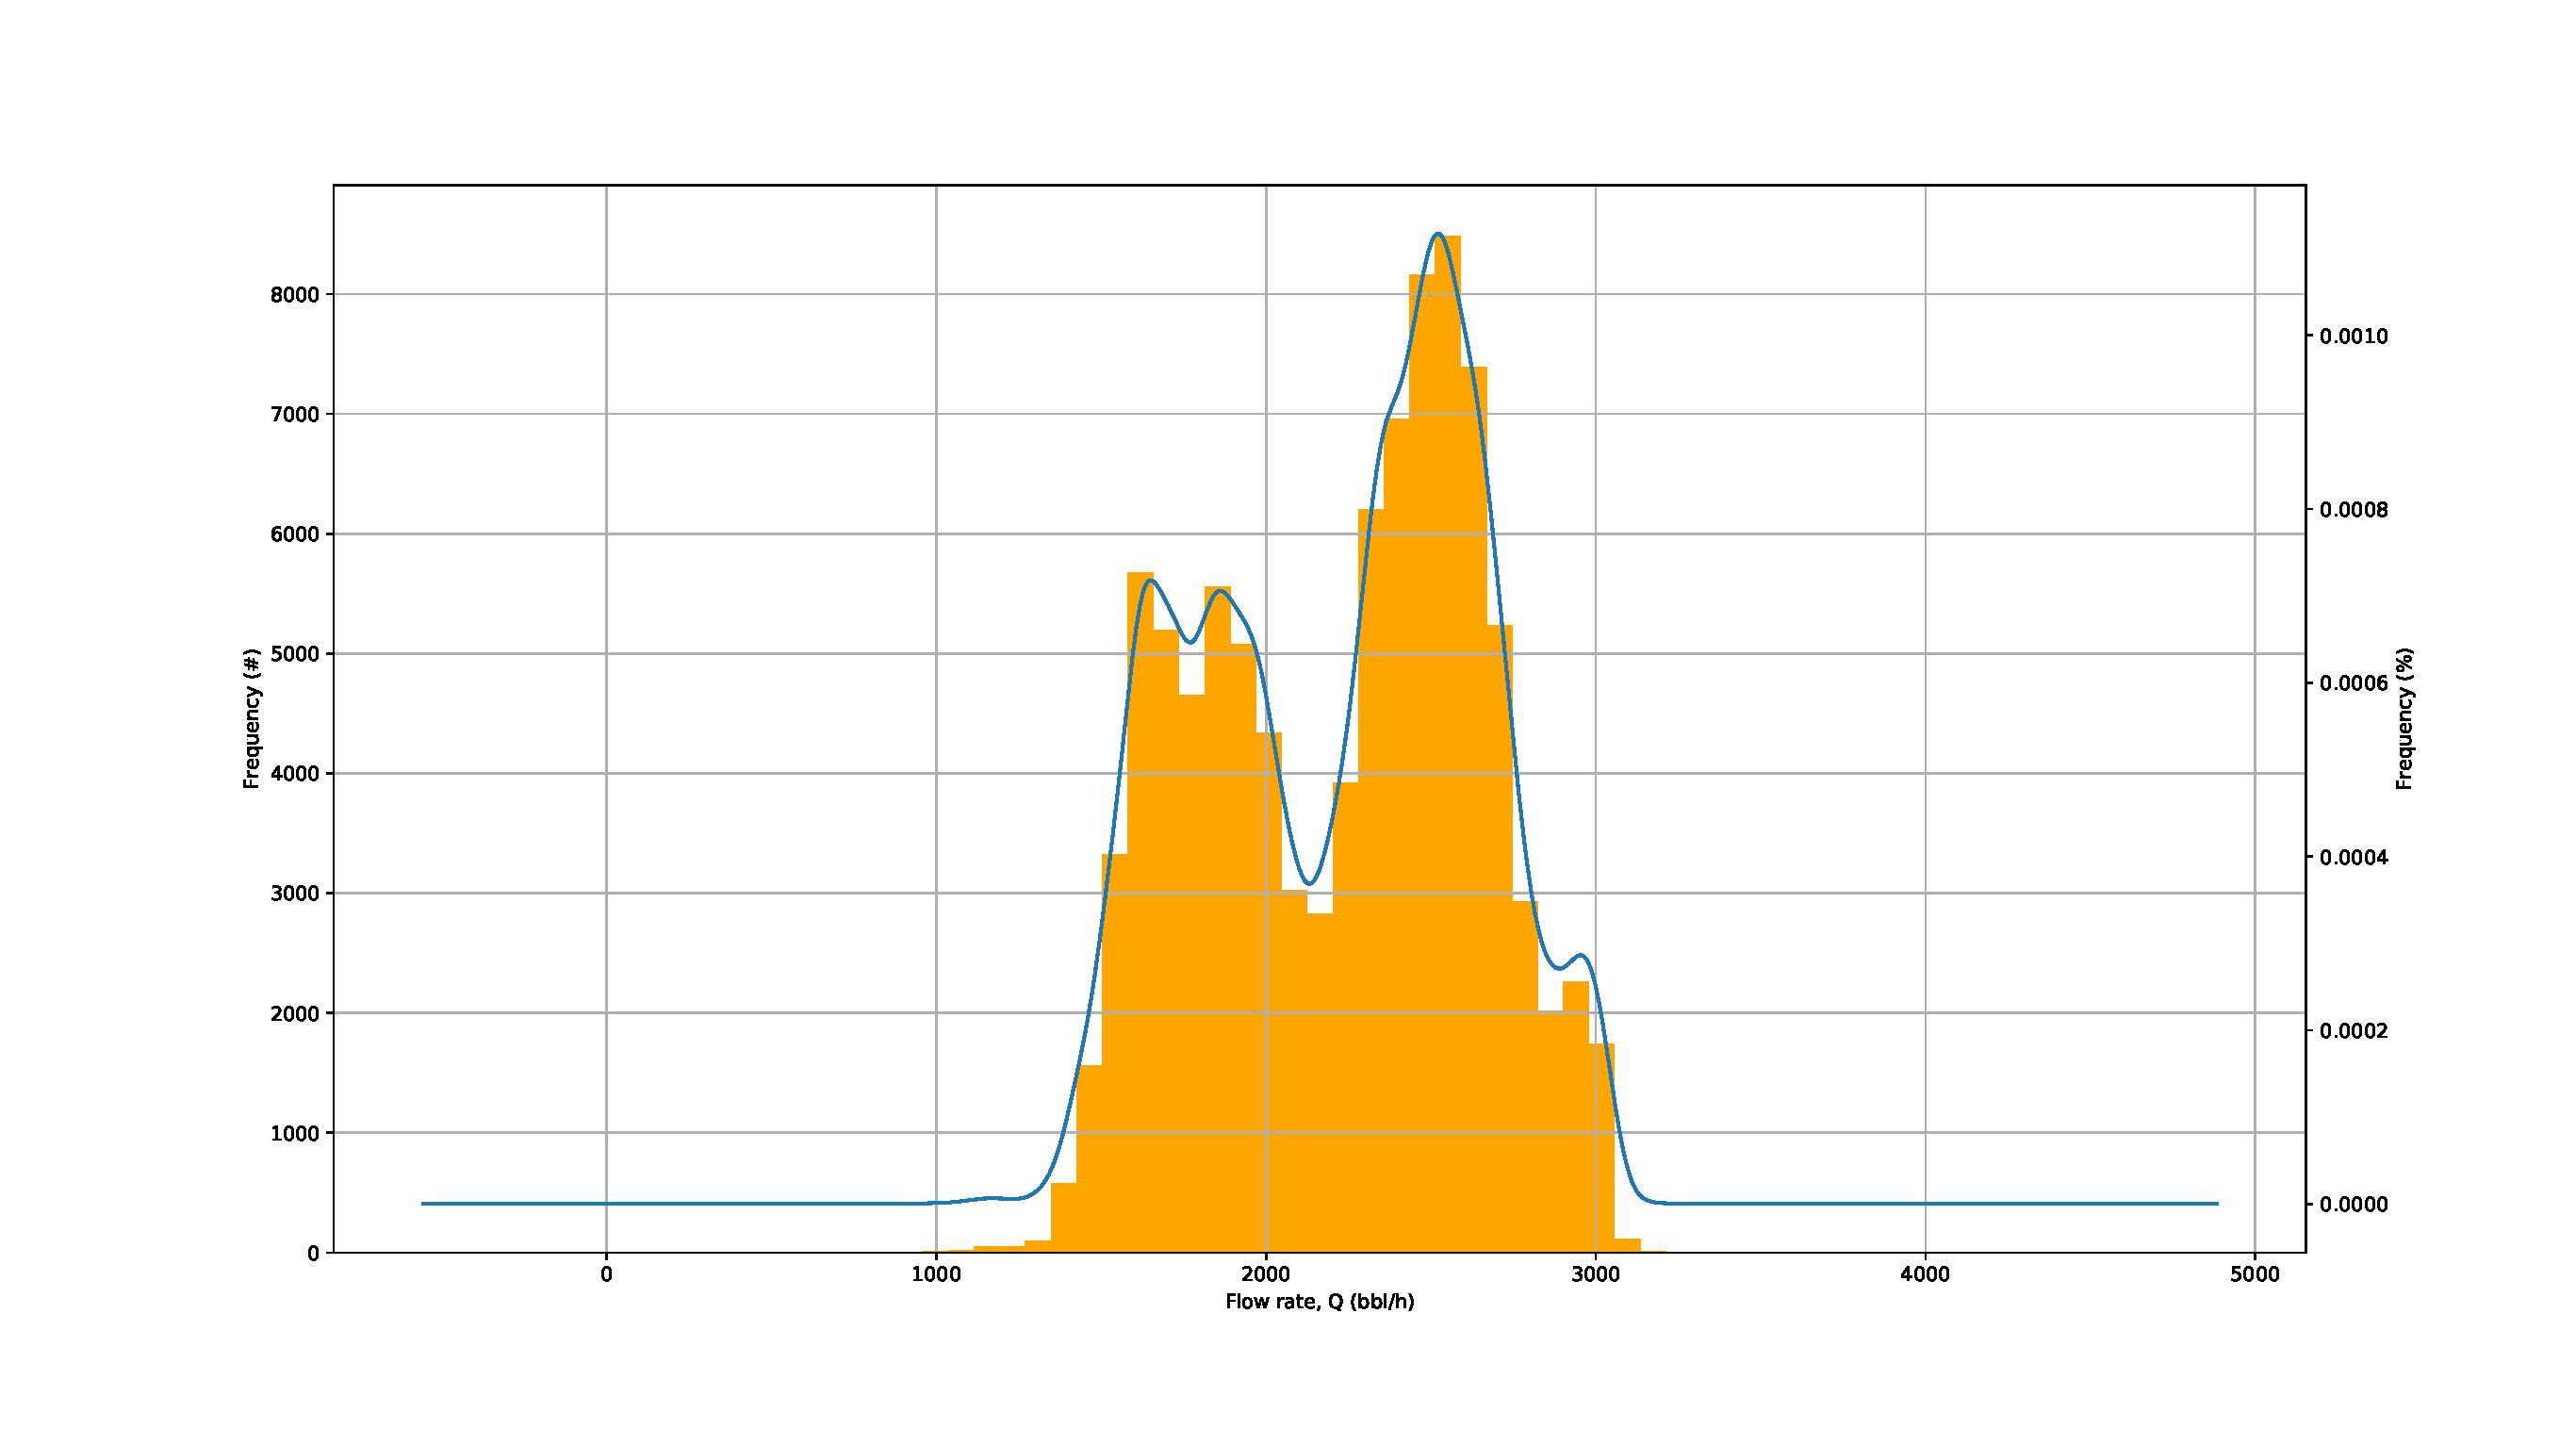
\includegraphics[scale=0.35]{images/08Flowrate_KDE.eps}
    \caption{Flow rate distribution of the pre-processed data set.}
    \label{fig:08flowrate_dist}
\end{figure}

To segregate the two Gaussian distributions, DBSCAN was used.  DBSCAN is a density-based algorithm for discovering clusters in large spatial data \cite{DBSCAN}. DBSCAN also scales much better to big data compared to affinity propagation or Gaussian mixture models due to the latter being iterative methods.
DBSCAN contains two hyper parameters, $\epsilon$ and $min \; points$.  The steps of DBSCAN is as follows:
\begin{enumerate}
    \item Normalize the data using Equation \ref{eq:08normalization} so each variable is weighted similarily.
    \item Create an $n-$dimensional sphere of radius $\epsilon$ around an initial data point.  Euclidean distance was used for the distance metric and is given by:
    \begin{equation}
        distance = \sqrt{(x_1^{(1)} - x_1^{(2)})^2 + (x_2^{(1)} - x_2^{(2)})^2 + ... + (x_m^{(1)} - x_m^{(2)})^2}
    \end{equation}
    where superscripts $1$ and $2$ denotes the first and second data points.
    \item If there are more than $min \; points$ in this sphere, then all points within this sphere belong to the same cluster.
    \item Expand the cluster by recursively applying the above criteria to the edge points of the cluster.
    \item If the cluster can no longer be expanded, apply steps 2 - 4 to a new data point currently not belonging to a cluster.
    \item If there are less than $min \; points$ in this sphere, then the data point is ignored and we proceed to the next data point.
    \item Outlier data points are ones that fail to belong to any cluster.
\end{enumerate}
The resultant segregation created by DBSCAN using hyper parameters 1.13 and 10,000 for $\epsilon$ and $min \; points$ is shown in Figure \ref{fig:08DBSCAN}. The first cluster (black) contained 56,738 data points while the second cluster (green) contained 36,779 data points.  The remaining 3953 data points (blue) were identified as outliers.
\begin{figure}[h]
    \centering
    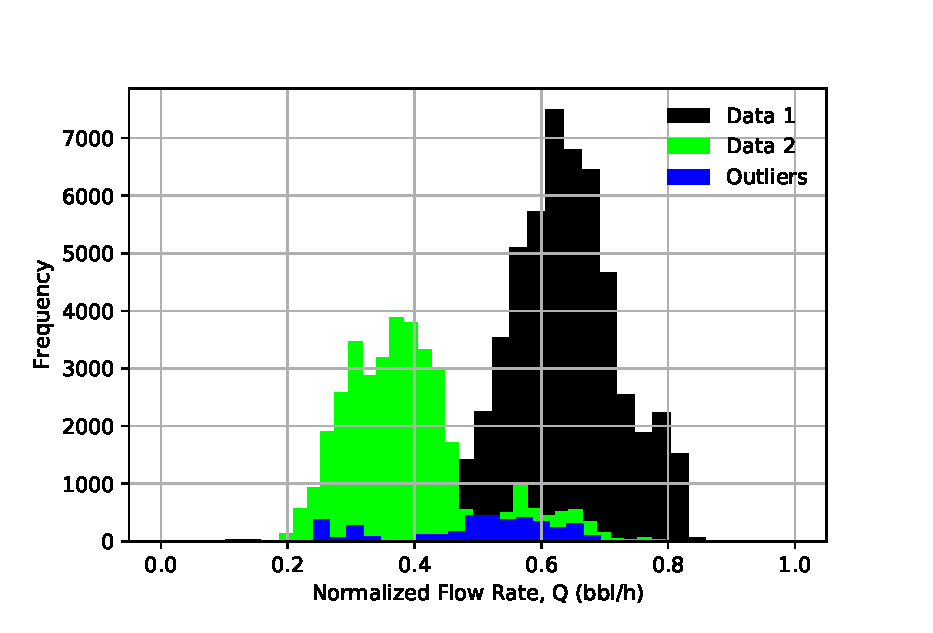
\includegraphics[scale=0.8]{images/08DBSCAN.eps}
    \caption{Clusters identified after applying the density-based scan.}
    \label{fig:08DBSCAN}
\end{figure}

The average operating conditions of each cluster is shown in Figure \ref{fig:08cluster_variables}. The main differences are the flow rate, DRA usage, and pump usage.  Cluster 1 had 32\% higher average flow rate.  Cluster 1 also used substantially more DRA compared to cluster 1, where almost no DRA was used. Furthermore, the Cheyenne booster pump, Ault booster pump 1, Fort Lupton boooster pump, and Fort Lupton VFD were only used in cluster 1.  Ault booster pump 2 was only used in cluster 2.
\begin{figure}
    \centering
    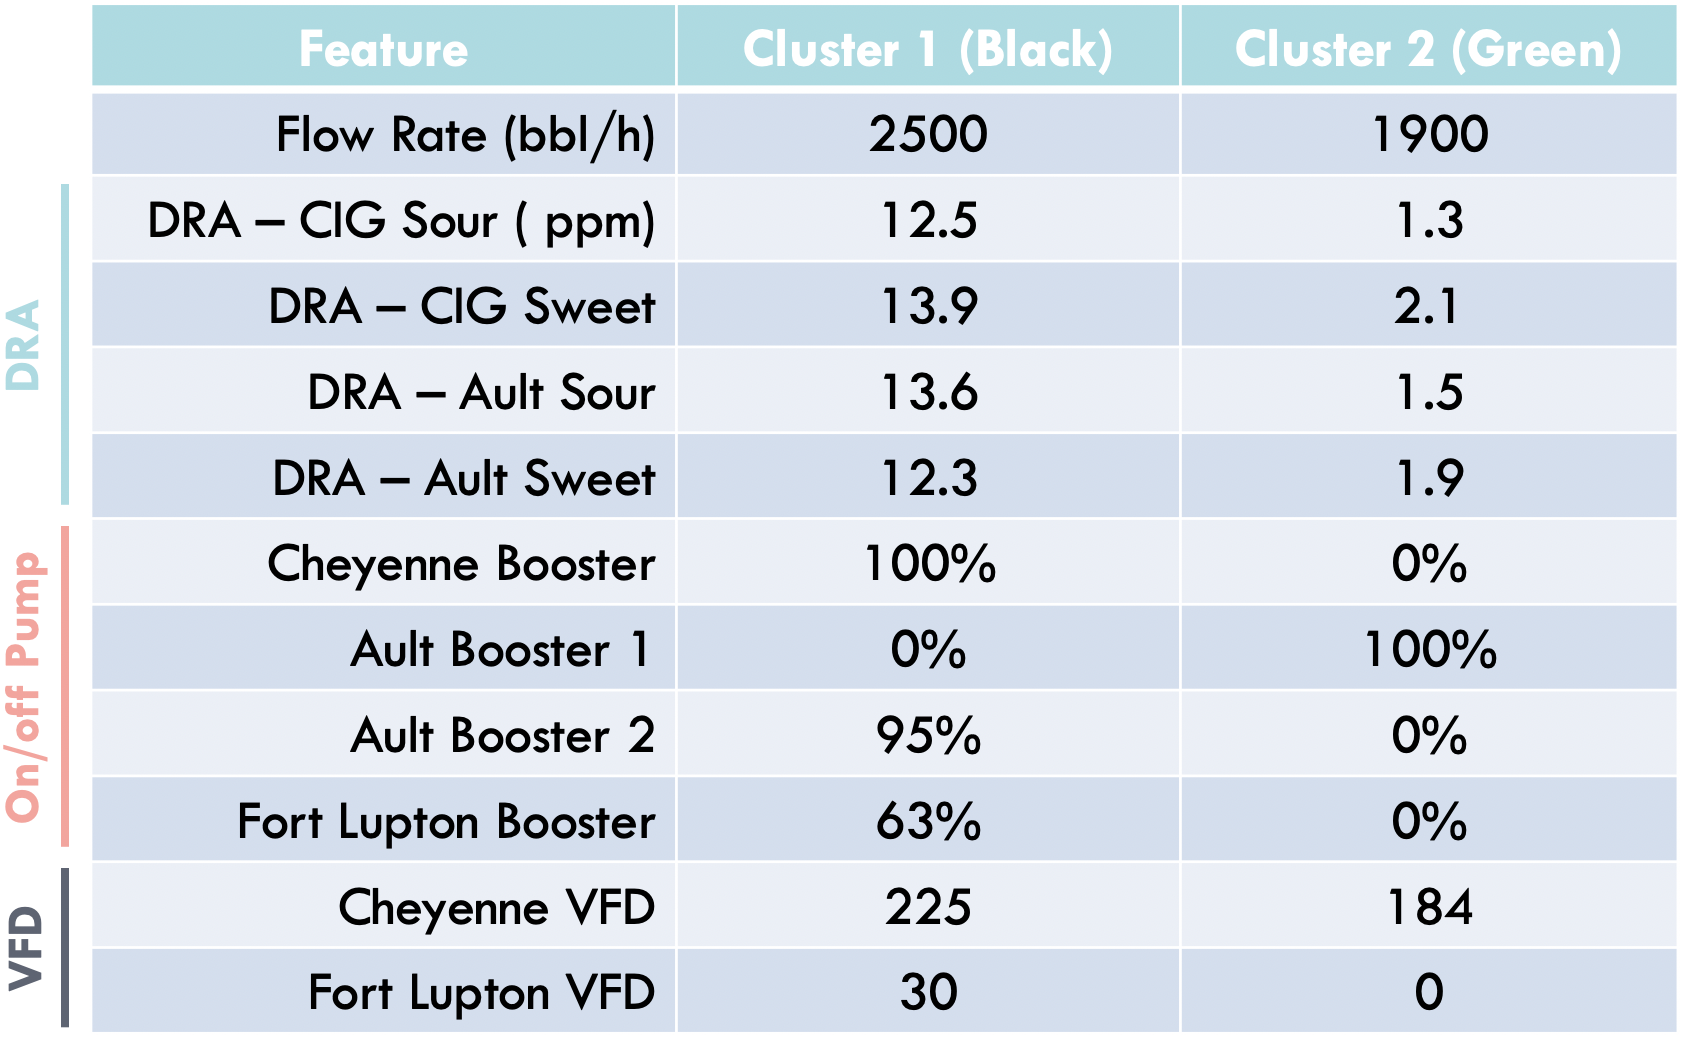
\includegraphics[width=0.8\textwidth]{images/08AvgChar.png}
    \caption{Average operating variables for the two operating conditions.}
    \label{fig:08cluster_variables}
\end{figure}

\subsubsection{Data Partitioning}
The data set was split into three sections for machine learning: training, validation, and testing.  The partition and description of each section is described in Table \ref{tab:08datapart}. The training data set was used to identify the machine learning model(s).  Then, the model was validated on unseen data via the validation data set (sometimes called development data).  The error of the model on the validation data set, $e_{validation}$, should be similar to the training data error, $e_{train}$, to ensure that the model did not overfit to the training data. Finally, the model will be tested on the testing data to explore the performance of the model in live production.  Testing data will always be the last 5\% of the data in the data set.
\begin{table}[h]
    \centering
    {\setstretch{1.2}
    \begin{tabular}{ c | c | p{9cm}}
                            & \% of Data        &  Description \\
        \hline
        Training            &  90\%             
        &  Used to identify the machine learning model        \\
        
        Validation          &  5\%              
        &  Validates the performance of the machine learning model         \\
        
        Testing             &  5\%             
        &  Used to test performance of machine learning model on unseen data       \\             
    \end{tabular}}
    \caption{Features selected for machine learning models.}
    \label{tab:08datapart}
\end{table}

\subsubsection{Cost Function}

The mean squared error (MSE) cost function was used for all predictive models and is given by:
\begin{equation}
    J(W) = \frac{1}{n}\sum\limits^n_{i=1}(\hat{y}_i - y_i)^2
    \label{eq:08MSE}
\end{equation}
where $n$ is the number of samples in the current optimization step.  $\hat{y}_i$ and $y_i$ are the $i^{th}$ predicted and actual labels, respectively. Here, $J$ is the loss. The MSE cost function was selected due to its convex nature \cite{deeplearning_course}.

To ensure adequate performance on the validation and testing data, the model must avoid overfitting to the training data.  This was done by reducing the model complexity through removing or reducing individual variables' impact on the model.  This study used a ridge regularization to reduce model complexity:
\begin{equation}
    J(W) = \frac{1}{n}\sum\limits^n_{i=1}(\hat{y}_i - y_i)^2 + \lambda \sum\limits^n_{j=1} W_j^2
    \label{eq:08MSE_wR}
\end{equation}
where $\lambda$ is the regularization penalty.  Here, as $\lambda \rightarrow \infty$, $W \rightarrow 0$.  That is, the larger $\lambda$ is, the stronger the weights are penalized. 

\subsubsection{Model Optimization}

The adaptive momentum (ADAM) gradient descent optimizer was used to update the weights and bias of the models.  The general gradient descent formulation is given by Equation \ref{eq:08GradientDescent} \cite{ADAM}.  
\begin{equation}
    \theta_j^{m+1} \leftarrow \theta_j^{m} - \alpha \frac{\partial J}{\partial \theta_j}
    \label{eq:08GradientDescent}
\end{equation}
where $\theta_j$ is the $j^{th}$ weight of the model.  Here, $m$ represents the $m^{th}$ update of gradient descent and $\alpha$ is the learning rate.  ADAM improves upon Equation \ref{eq:08GradientDescent} by computing an adaptive learning rate for each parameter. To do so, the exponentially decaying average of the past gradients and squared gradients of the weights and biases are computed and stored using Equations \ref{eq:08momentW} to \ref{eq:08squared_momentb}.
\begin{equation}
    V_{dW} = \beta_1 V_{dW} + (1 - \beta_1)dW
    \label{eq:08momentW}
\end{equation}
\begin{equation}
    V_{db} = \beta_1 V_{db} + (1 - \beta_1)db
    \label{eq:08momentb}
\end{equation}
\begin{equation}
    S_{dW} = \beta_2 S_{dW} + (1 - \beta_2)dW^2
    \label{eq:08squared_momentW}
\end{equation}
\begin{equation}
    S_{db} = \beta_2 S_{db} + (1 - \beta_2)db^2
    \label{eq:08squared_momentb}
\end{equation}
where $V$ and $S$ are the estimates of the gradient and squared gradients, respectively.  $V$ and $S$ are typically initiated as zero vectors and are heavily biased towards zero at initial steps.  Hence, the biases for the initial terms are corrected using:
\begin{equation}
    V_{dW}^{corrected} = \frac{V_{dW}}{1 - \beta_1^t}
\end{equation}
\begin{equation}
    V_{db}^{corrected} = \frac{V_{db}}{1 - \beta_1^t}
\end{equation}
\begin{equation}
    S_{dW}^{corrected} = \frac{S_{dW}}{1 - \beta_2^t}
\end{equation}
\begin{equation}
    S_{db}^{corrected} = \frac{S_{db}}{1 - \beta_2^t}
\end{equation}
Combining the above equations, the weights and biases are updated by:
\begin{equation}
    W_j \leftarrow W_j - \alpha \frac{V_{dW}^{corrected}}{S_{dW}^{corrected} + \epsilon}
\end{equation}
\begin{equation}
    b \leftarrow b - \alpha \frac{V_{db}^{corrected}}{S_{db}^{corrected} + \epsilon}
\end{equation}
where $\epsilon$ is a small scalar to avoid division by zero. The authors proposed values of 0.9, 0.999 and $10^{-8}$ for $\beta_1$, $\beta_2$, and $\epsilon$, respectively.

Due to the size of the data, batch gradient descent where all data are used to compute the gradient at each step is computationally infeasible.  Thus, mini-batch gradient descent was used where smaller batches of data were sampled from the original data set to perform stochastic updates at each step.
\subsubsection{Performance Assessment}
The model performance were assessed using the following three ways:
\begin{enumerate}
    \item Root mean squared error (RMSE):
    \begin{equation}
        J = \sqrt{\frac{1}{n}\sum\limits^n_{i=1}(\hat{y}_i - y_i)^2}
        \label{eq:08RMSE}
    \end{equation}
    
    \item Mean absolute error (MAE):
    \begin{equation}
        J = \frac{1}{n}\sum\limits^n_{i=1}|\hat{y}_i - y_i|
        \label{eq:08MSE_Error}
    \end{equation}
    \item Coefficient of determination ($R^2$):
    \begin{equation}
        R^2 = 1 - \frac{\sum\limits^n_{i = 1}(\hat{y_i} - y_i)^2}{\sum\limits^n_{i = 1}(y_i - \bar{y_i})^2}
    \end{equation}
\end{enumerate}
Table \ref{tab:08performanceassessment} shows the advantages and disadvantages of each assessment metric.
\begin{table}[h]
    \centering
    {\setstretch{1.2}
    \begin{tabular}{ c | p{7cm} | p{7cm}}
         Method             & Advantages        &  Disadvantages \\
        \hline
        RMSE                &  Useful for identifying large errors                            &  Smaller errors are muted        \\
        
        MAE                 &  Easy to interpret as all errors have the same weight           &  Inferior to RMSE when large errors are undesirable \\
        
        $R^2$               &  Easy to understand, $-\infty \leq R^2 \leq 1$                                         &  Valid only for linear relationships       \\             
    \end{tabular}}
    \caption{Constrained least squares validation and test plots.}
    \label{tab:08performanceassessment}
\end{table}

%%%%%%%%%%%%%%%%%%%%%%%%%%%%%%%%%%%%%%%%%%%%%%%%%%%%%%%%%%%%%%%%%%%%%
%
% Least squares model
%
%%%%%%%%%%%%%%%%%%%%%%%%%%%%%%%%%%%%%%%%%%%%%%%%%%%%%%%%%%%%%%%%%%%%%
\subsubsection{Linear Modelling}
\noindent
\textit{Linear Regression} \\
Linear regression was the first regression method to be explored, and was selected as the benchmark due to its simplicity and linear nature. The model structure of linear regression is given as:
\begin{equation}
    \hat{y} = W_1^Tx + W_2^Tu + b
    \label{eq:08LS}
\end{equation}
where $x \in R^8$ is a vector of states, $u \in R^{10}$ is a vector of inputs and superscript $T$ denotes the transpose operation.

Hyper parameters of the linear regression are shown in Table \ref{tab:08LSHparameters}.
\begin{table}[h]
    \centering
    {\setstretch{1.2}
    \begin{tabular}{ c | c}
        Hyper Parameter                  &  Value       \\
        \hline
        Epochs                           &  800      \\
        Minibatch size                   &  8192     \\
        Learning rate, $\alpha$          &  0.001    \\
        Regularization, $\lambda$          &  0.001  \\
    \end{tabular}}
    \caption{Hyper parameters for linear regression.}
    \label{tab:08LSHparameters}
\end{table}

The performance assessment of the least squares model is shown in Table \ref{tab:08LSperformance}. Error on the test data was 5.8\% higher compared to the training and validation data.
\begin{table}[h]
    \centering
    {\setstretch{1.2}
    \begin{tabular}{ c | c | c | c}
                             &  Training data    &  Validation data   &    Test data      \\
        \hline
        MAE                  &  98               &    98              &  102     \\
        RMSE                 &  127              &   127              &  135    \\ 
        $R^2$                &  0.91             &   0.91             &  0.70   \\
    \end{tabular}}
    \caption{Performance assessment for the linear regression.}
    \label{tab:08LSperformance}
\end{table}

The model performance on the validation and test data sets are shown in Figures \ref{fig:08LSValidation} and \ref{fig:08LSTest}.
\begin{figure}[h]
     \centering
     \begin{subfigure}[b]{0.48\textwidth}
         \centering
         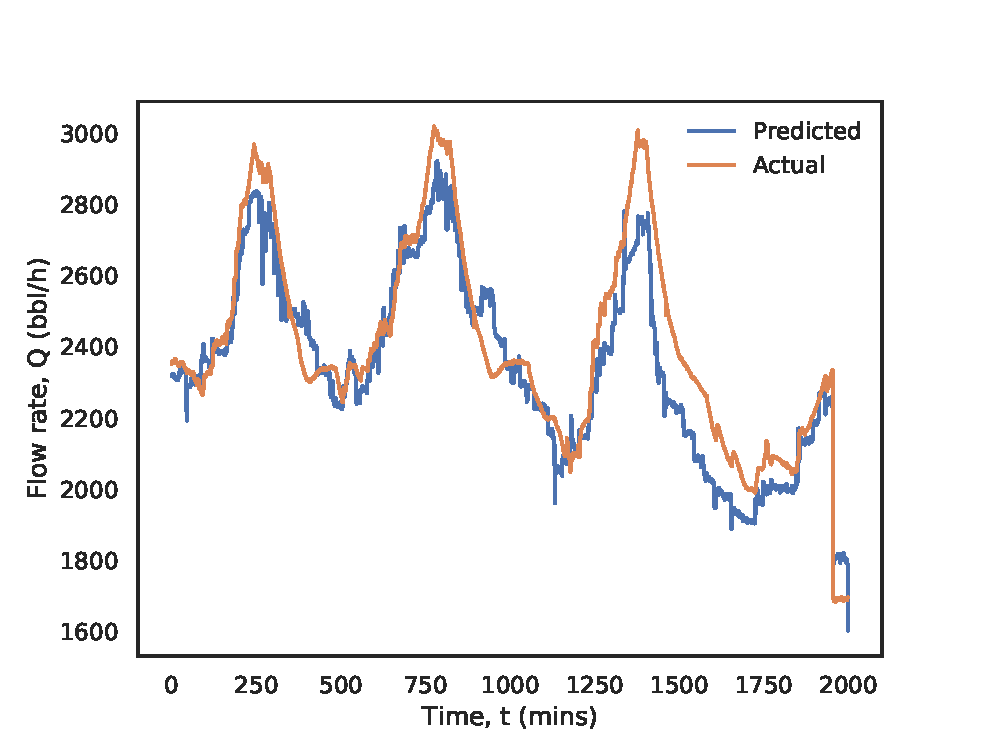
\includegraphics[width=\textwidth]{images/08ls_validation.eps}
         \caption{Predicted vs. actual flow rate for the validation data set.}
         \label{fig:08LSValidation}
     \end{subfigure}
     \hfill
     \begin{subfigure}[b]{0.48\textwidth}
         \centering
         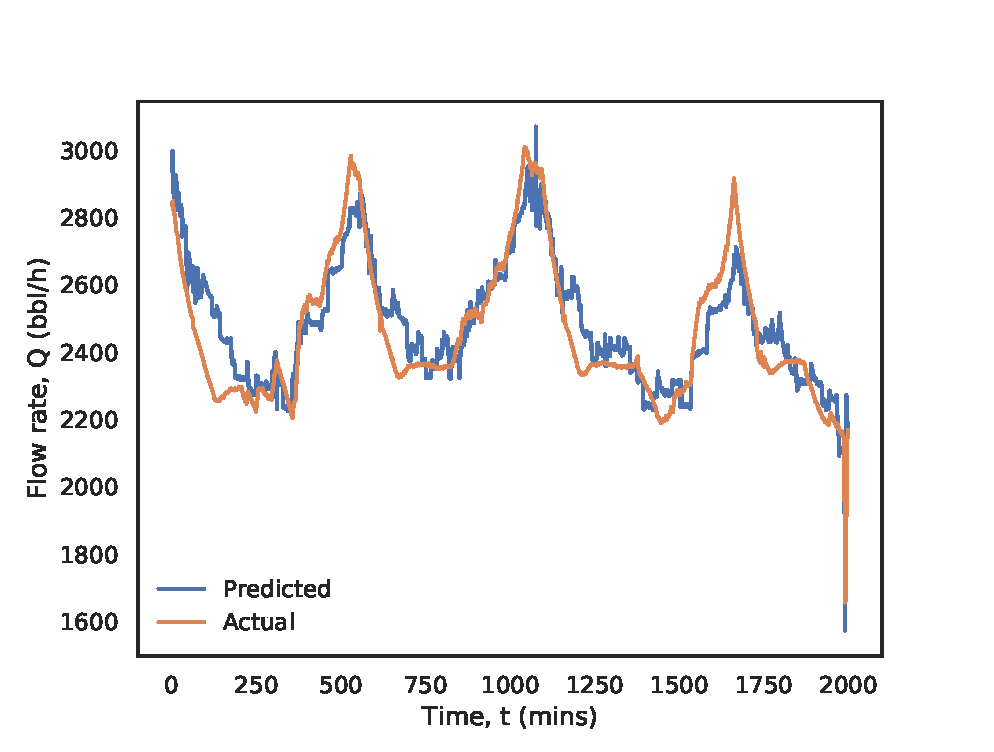
\includegraphics[width=\textwidth]{images/08ls_test.eps}
         \caption{Predicted vs. actual flow rate for the test data set.}
         \label{fig:08LSTest}
     \end{subfigure}
        \caption{Comparison of normal and abnormal density readings.}
        \label{fig:08LSPlots}
\end{figure}

The linear regression model is given in Equation \ref{eq:08LS}.  Weights for $x_{1} - x_{4}$ were very small and were omitted.
\begin{multline}
    \hat{y} = 0.10u_1 + 0.15u_2 + 0.13u_3 + 0.04u_4 + 0.04u_5 + 0.09u_6 + 0.12u_7 - 0.01u_8 \\
    + 0.49u_9 + 0.02u_{10} + 0.09x_{1} - 0.18x_{5} + 0.30x_{6} - 0.05x_{7} + 0.04x_{8}
    \label{eq:08LS_eq}
\end{multline}

From Equation \ref{eq:08LS}, it can be seen that turning on the booster pump at Fort Lupton results in a decrease in flow rate.  Theoretically, this is impossible and is most likely caused by noise in the data.  To increase the model's ability to reflect reality, engineering knowledge was injected into the model via constraining the weights of $u_1 - u_{10}$ to be strictly positive.

%%%%%%%%%%%%%%%%%%%%%%%%%%%%%%%%%%%%%%%%%%%%%%%%%%%%%%%%%%%%%%%%%%%%%
%
% Constrained LS
%
%%%%%%%%%%%%%%%%%%%%%%%%%%%%%%%%%%%%%%%%%%%%%%%%%%%%%%%%%%%%%%%%%%%%%

\noindent
\textit{Constrained Linear Regression} \\
\indent
The constrained linear regression used the same hyper parameters as shown in Table \ref{tab:08LSHparameters}.  Performance assessment of the constrained linear regression is shown in Table \ref{tab:08ConstLSPerformance}. Compared to the original linear regression, RMSE increased by 0.8\% for the training and validation data sets.  However, performance on the test set was improved by 8\%.  
\begin{table}[h]
    \centering
    {\setstretch{1.2}
    \begin{tabular}{ c | c | c | c}
                             &  Training data    &  Validation data   &    Test data      \\
        \hline
        MAE                  &  98               &    98              &  94     \\
        RMSE                 &  128              &   129              &  123    \\ 
        $R^2$                &  0.91             &   0.91             &  0.74   \\
    \end{tabular}}
    \caption{Performance assessment for the constrained linear regression.}
    \label{tab:08ConstLSPerformance}
\end{table}
The constrained linear regression performance on the validation and test data sets are shown in Figures \ref{fig:08CLSValidation} and \ref{fig:08CLSTest}. The weights were nearly identical to the unconstrained model; however, all negative weights on operating variables were removed.
\begin{figure}[h]
     \centering
     \begin{subfigure}[b]{0.48\textwidth}
         \centering
         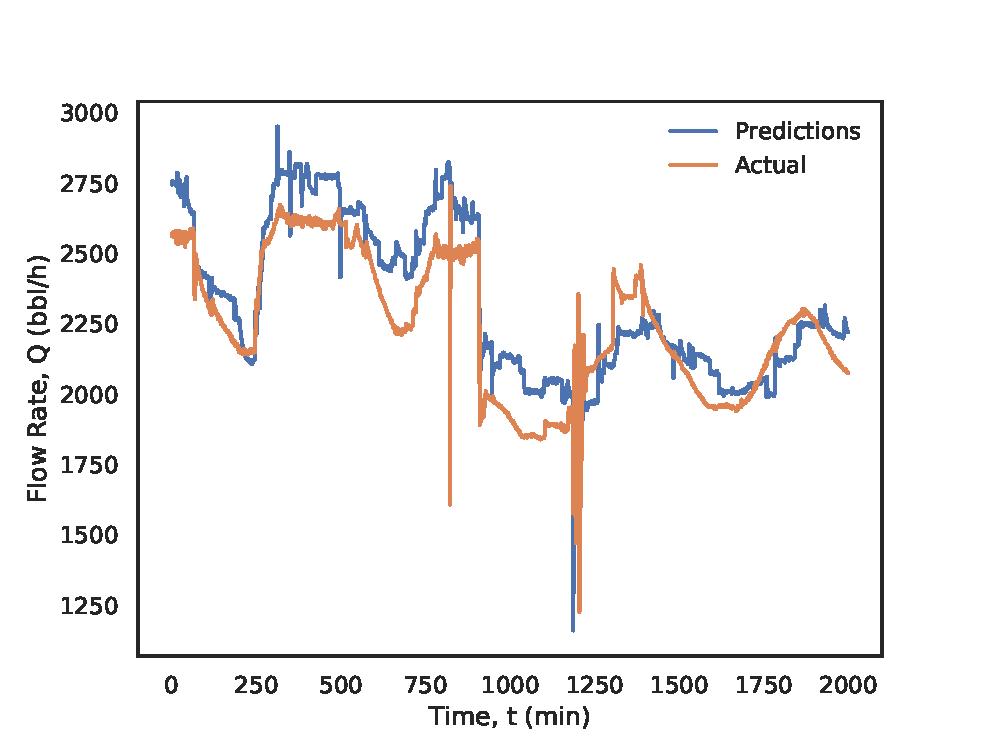
\includegraphics[width=\textwidth]{images/08ConstrainedLS_validation.eps}
         \caption{Predicted vs. actual flow rate for the validation data set.}
         \label{fig:08CLSValidation}
     \end{subfigure}
     \hfill
     \begin{subfigure}[b]{0.48\textwidth}
         \centering
         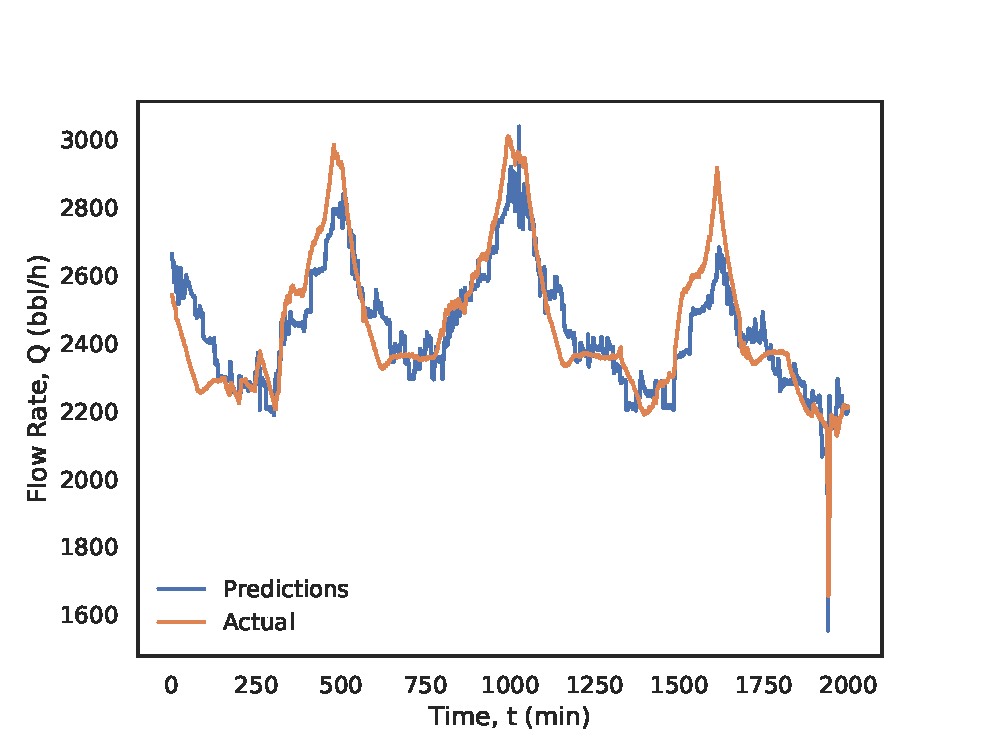
\includegraphics[width=\textwidth]{images/08ConstrainedLS_test.eps}
         \caption{Predicted vs. actual flow rate for the test data set.}
         \label{fig:08CLSTest}
     \end{subfigure}
        \caption{Constrained linear regression validation and test plots.}
        \label{fig:08CLSPlots}
\end{figure}

The constrained linear regression is given in Equation \ref{eq:08CLS}.  Weights for $x_{8}, x_{11} - x_{14}$ were very small and were omitted.
\begin{multline}
    \hat{y} = 0.10x_1 + 0.15x_2 + 0.13x_3 + 0.04x_4 + 0.04x_5 + 0.09x_6 + 0.11x_7 \\
    + 0.49x_9 + 0.02x_{10}  - 0.18x_{15} + 0.30x_{16} - 0.05x_{17} + 0.03x_{18}
    \label{eq:08CLS}
\end{multline}

\subsubsection{Non-linear Modelling}
To further increase the accuracy of the models, the following non-linear methods were explored for modelling the pipeline flow rate:
\begin{itemize}
    \item Polynomial models
    \begin{itemize}
        \item Quadratic model
        \item Square-root model
    \end{itemize}
    \item Feed-forward neural networks
    \begin{itemize}
        \item Small neural network (3 layers, 20 nodes per layer)
        \item Medium neural network (6 layers, 30 nodes per layer)
        \item Large neural network (8 layers, 40 nodes per layer)
    \end{itemize}
    \item Linear parameter-varying model
\end{itemize}

Performance assessment of the non-linear models will use MAE and RMSE. In non-linear models, $R^2$ is not valid due to $SS_R + SS_E \neq SS_{Total}$ and was not provided \cite{generic_stats}.
%%%%%%%%%%%%%%%%%%%%%%%%%%%%%%%%%%%%%%%%%%%%%%%%%%%%%%%%%%%%%%%%%%%%%
%
%  Quadratic and Sqrt models
%
%%%%%%%%%%%%%%%%%%%%%%%%%%%%%%%%%%%%%%%%%%%%%%%%%%%%%%%%%%%%%%%%%%%%%
\noindent
\textit{Polynomial Models} \\
The quadratic and square-root model structures are given by Equations \ref{eq:08quad_model} and \ref{eq:08sqrt_model}, respectively:
\begin{equation}
    \hat{y} = W_1^T X^2 + W^T_2 X + b
    \label{eq:08quad_model}
\end{equation}
\begin{equation}
    \hat{y} = W_1^T X^{1/2} + W^T_2 X + b
    \label{eq:08sqrt_model}
\end{equation}
where $W_1 \in R^{18}$ are the weights for the squared and square rooted variables for the quadratic and square root models, respectively. Furthermore, $W_2 \in R^{18}$ are the weights for the original variables. The hyper parameters for both models are shown in Table \ref{tab:08poly_hp}.
\begin{table}[h]
    \centering
    {\setstretch{1.2}
    \begin{tabular}{ c | c}
        Hyper Parameter                  &  Value       \\
        \hline
        Epochs                           &  1000      \\
        Minibatch size                   &  8192     \\
        Learning rate, $\alpha$          &  0.001    \\
        Regularization, $\lambda$          &  0.001  \\
    \end{tabular}}
    \caption{Hyper parameters for polynominal regression.}
    \label{tab:08poly_hp}
\end{table}

The performance assessment of the quadratic and square root models are shown in Table \ref{tab:08quad_sqrt_performance}. Compared to linear regression, MAE and RMSE reduced by up to 10\% and 9\% when using the polynomial models, respectively. Moreover, performance of the square root model was about 3.5\% better than the quadratic model.
\begin{table}[h]
    \centering
    {\setstretch{1.2}
    \begin{tabular}{c|c|c|c|c|c|c|}
      & \multicolumn{2}{c|}{Training data} & \multicolumn{2}{c|}{Validation data} & \multicolumn{2}{c|}{Test data} \\ \cline{2-7} 
      & Quad             & Sqrt            & \multicolumn{1}{c|}{Quad}   & Sqrt   & Quad           & Sqrt          \\ \hline
    MAE   & 92               & 89              & 92                          & 89     & 89             & 91            \\
    RMSE  & 121              & 118             & \multicolumn{1}{c|}{121}    & 117    & 120            & 115           \\
    \end{tabular}}
    \caption{Performance assessment for the quad. and sqrt. model.}
    \label{tab:08quad_sqrt_performance}
\end{table}

The polynomial models' performance on the validation and test data are shown in Figures \ref{fig:08quad_validation} to \ref{fig:08sqrt_test}.  

\newpage
\begin{figure}[h]
     \centering
     \begin{subfigure}[b]{0.45\textwidth}
         \centering
         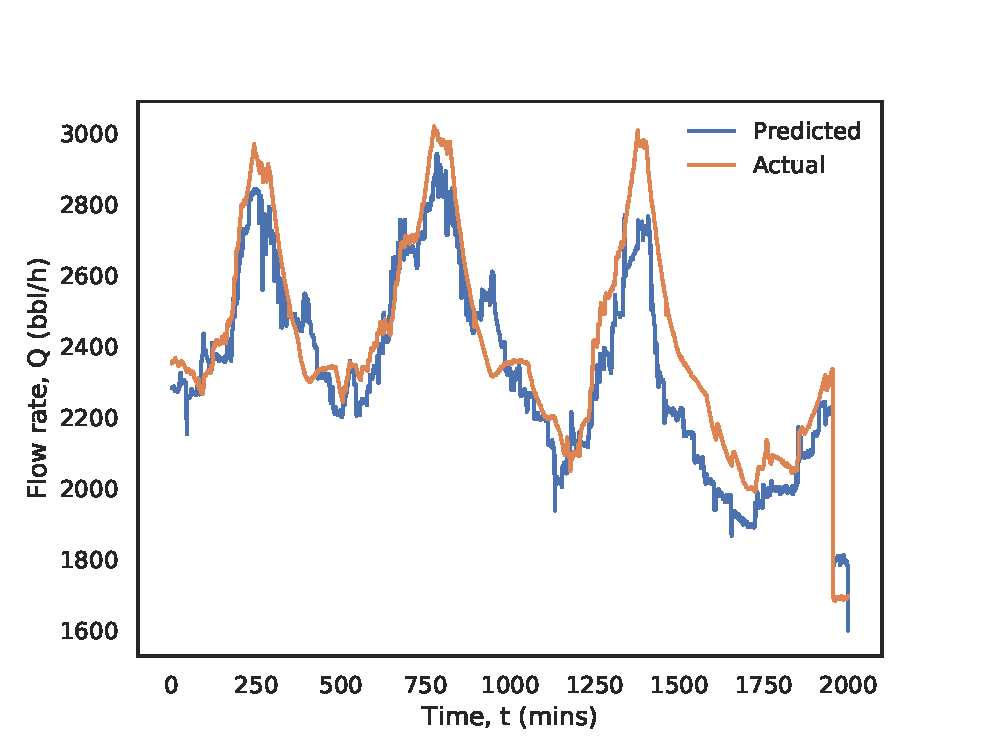
\includegraphics[width=\textwidth]{images/08quad_validation.eps}
         \caption{Predicted vs. actual flow rate for validation data using the quad. model.}
         \label{fig:08quad_validation}
     \end{subfigure}
     \begin{subfigure}[b]{0.45\textwidth}
         \centering
         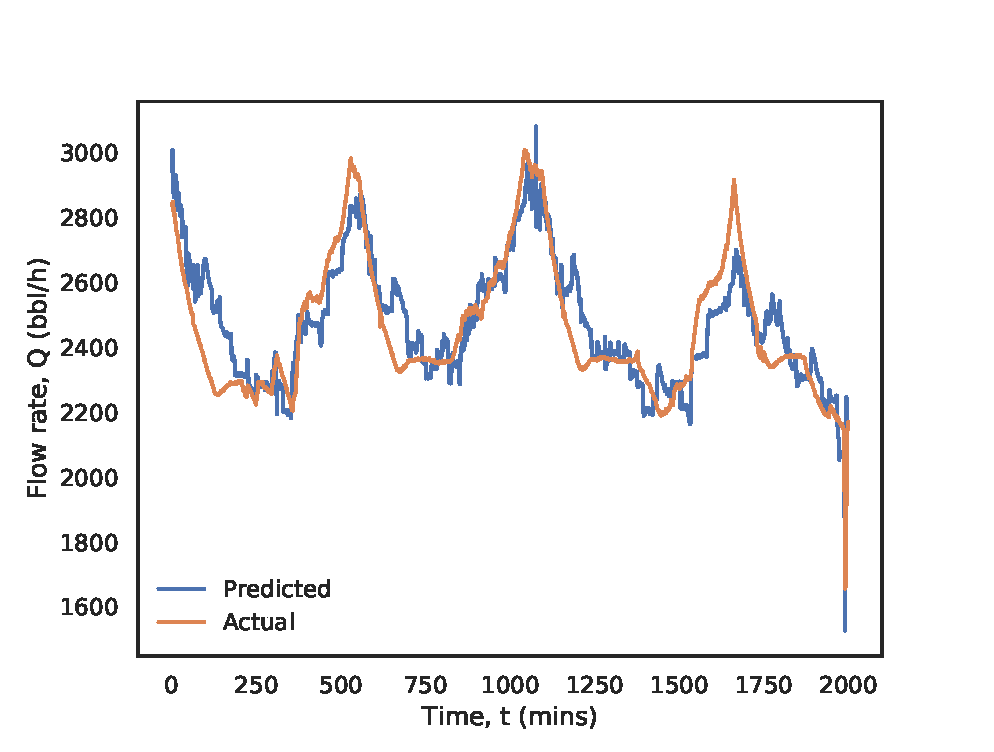
\includegraphics[width=\textwidth]{images/08quad_test.eps}
         \caption{Predicted vs. actual flow rate for the test data using the quadratic model.}
         \label{fig:08quad_test}
     \end{subfigure}
     \begin{subfigure}[b]{0.45\textwidth}
         \centering
         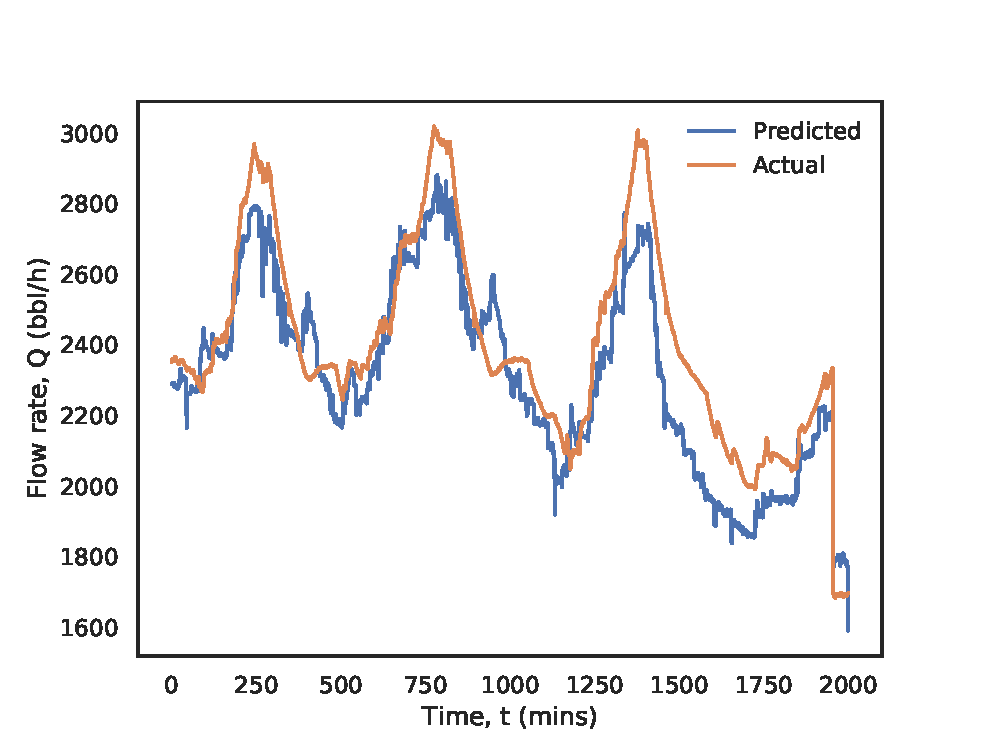
\includegraphics[width=\textwidth]{images/08sqrt_validation.eps}
         \caption{Predicted vs. actual flow rate for the validation data using the sqrt. model.}
         \label{fig:08sqrt_validation}
     \end{subfigure}
     \begin{subfigure}[b]{0.45\textwidth}
         \centering
         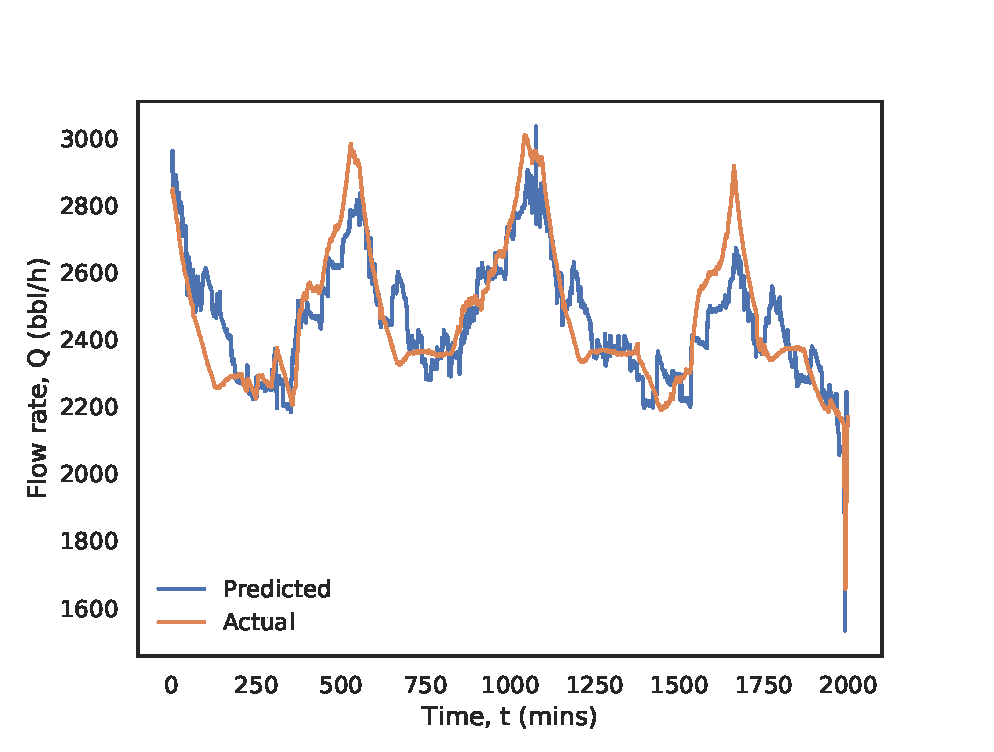
\includegraphics[width=\textwidth]{images/08sqrt_test.eps}
         \caption{Predicted vs. actual flow rate for the test data using the sqrt. model.}
         \label{fig:08sqrt_test}
     \end{subfigure}
        \caption{Polynomial regression validation and test plots.}
        \label{fig:08PolynomialPlots}
\end{figure}

%%%%%%%%%%%%%%%%%%%%%%%%%%%%%%%%%%%%%%%%%%%%%%%%%%%%%%%%%%%%%%%%%%%%%
%
% Neural Network Models
%
%%%%%%%%%%%%%%%%%%%%%%%%%%%%%%%%%%%%%%%%%%%%%%%%%%%%%%%%%%%%%%%%%%%%%
\noindent
\textit{Neural Network Models} \\
Neural networks are highly non-linear models that explore the individual and interaction effects of each variable with all other variables. The general structure of a neural network is shown in Figure \ref{fig:08NN}.  Neural networks are comprised of an input layer, some hidden layer(s), and an output layer.  The input layer consists of the input data, while the hidden layer(s) and output layer consists of fitted parameters, $W_{n_x \times n_b}$ and $b_{n_b \times 1}$. Here, $n_b$ and $n_x$ denotes the batch size and the dimension of the input layer, respectively. In Figure \ref{fig:08NN}, $x_m$ denotes the $m^{th}$ input variable.  The superscript and subscript of $a$ denotes the hidden layer number and the node number in the corresponding layer, respectively.  Subscript $m_1$ to $m_r$ denotes the number of nodes in hidden layers 1 to $r$, respectively.  Finally, superscript $o$ denotes the output layer.
\begin{figure}[h]
    \centering
    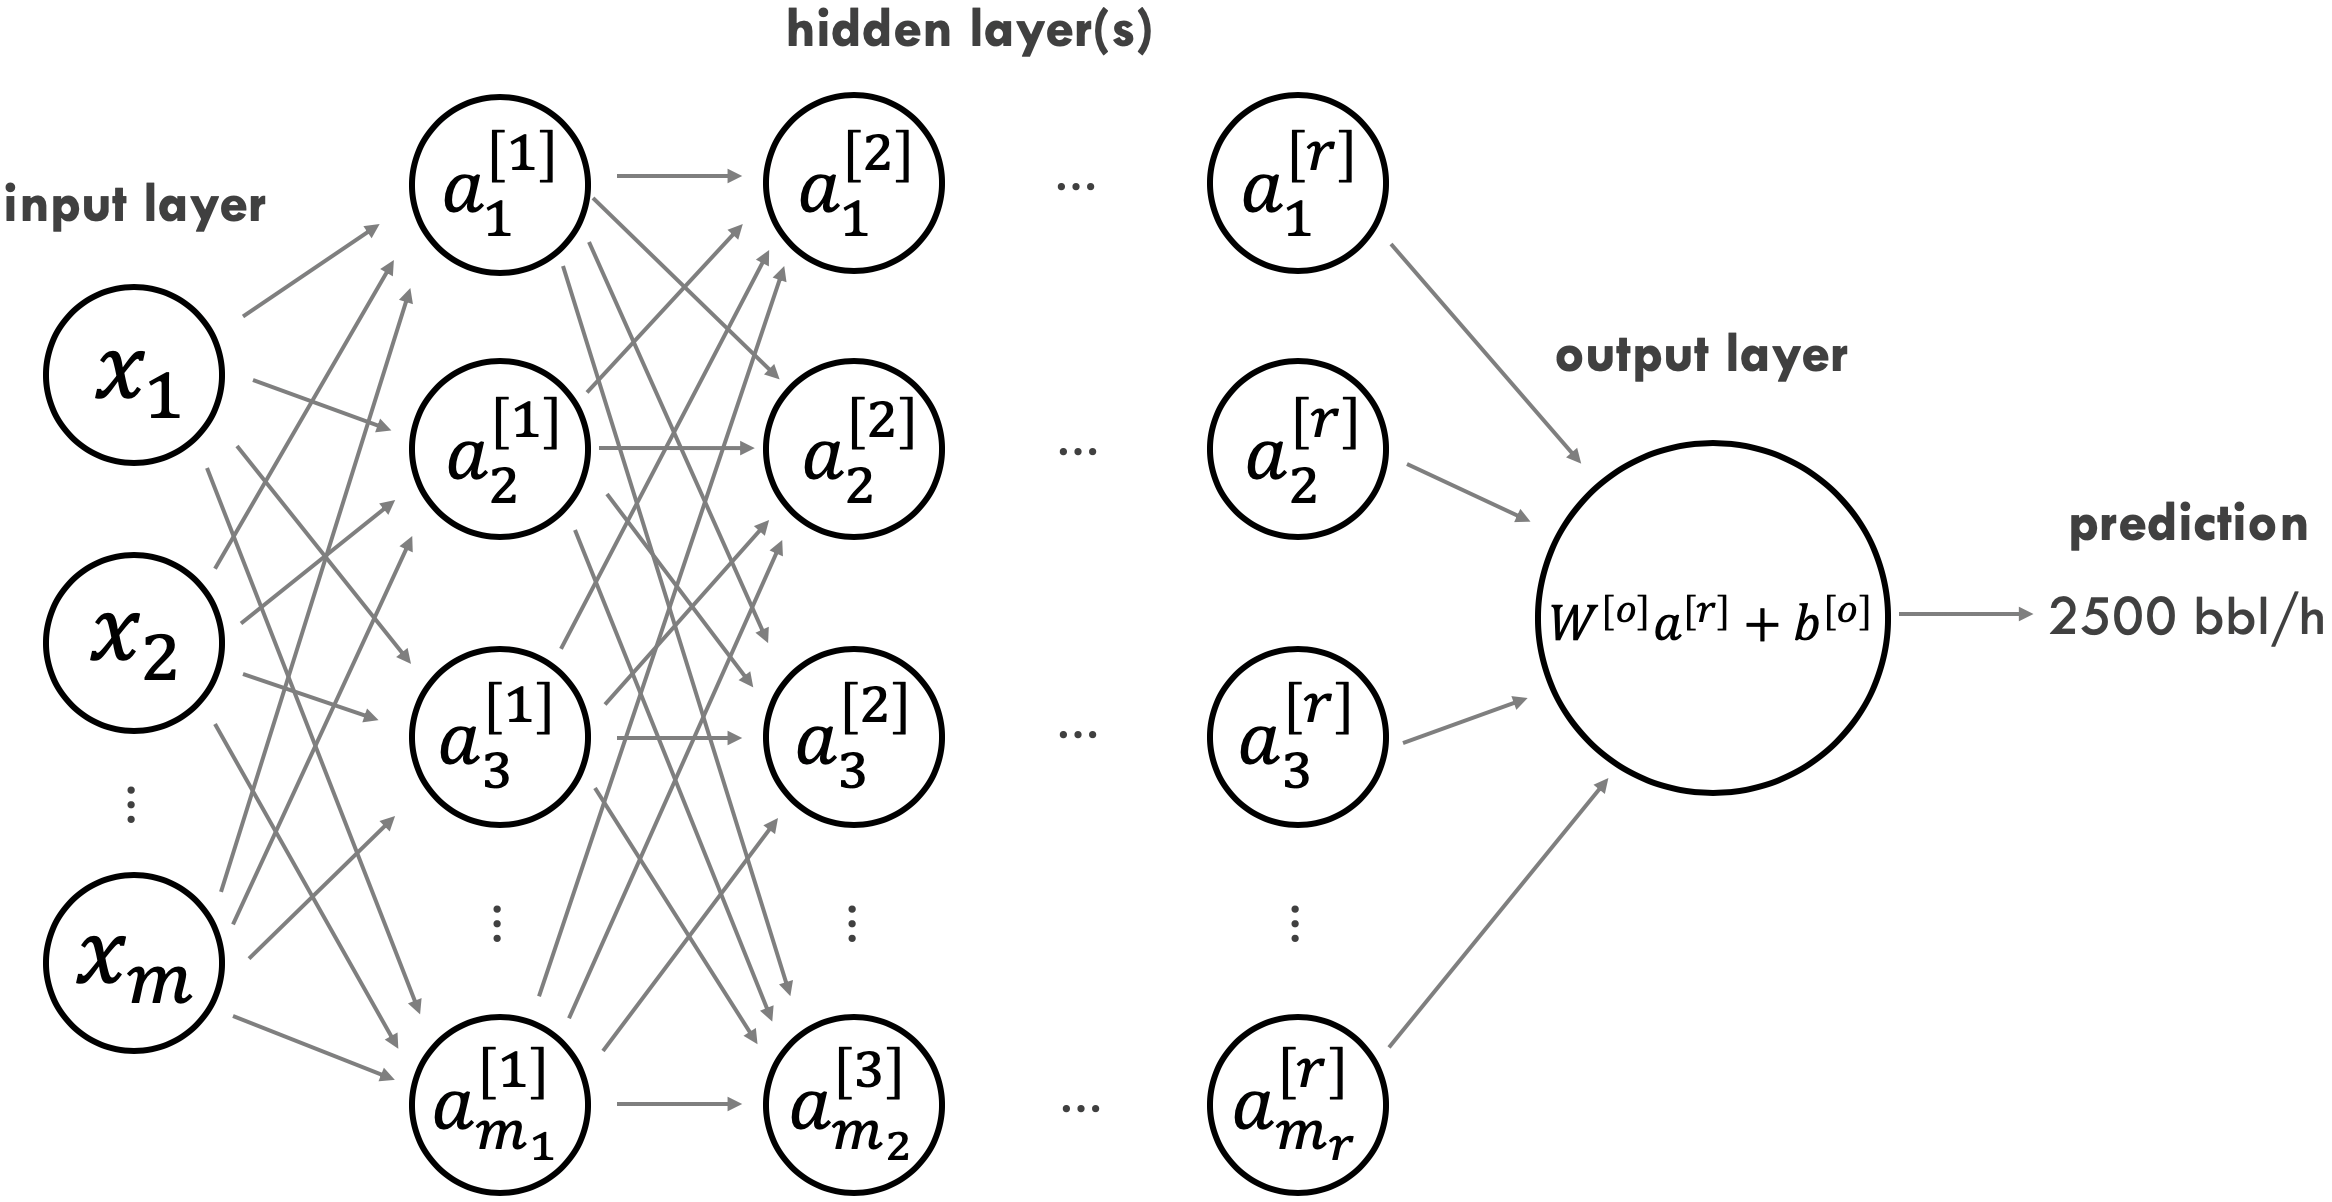
\includegraphics[width=0.9\textwidth]{images/08NN.png}
    \caption{Structure of a general neural network.}
    \label{fig:08NN}
\end{figure}

The details within a hidden layer's node is shown in Figure \ref{fig:08NNNode}. First, the outputs from the previous layer's nodes are inputted and multiplied by the weights of the current node.  The current node's bias is then added. If the current node is in the first layer, the outputs from the previous layer is replaced with the input variables. Afterwards, the output is sent to a rectified linear unit (ReLU) activation function given by:
\begin{equation}
    a^{[i]}_j=\begin{cases}
        y, & \text{if $y\geq0$}.\\
        0, & \text{otherwise}.
    \end{cases}
    \label{eq:08ReLU}
\end{equation}
where $i$ and $j$ denotes any hidden layer and any node number, respectively.  
\begin{figure}[h]
    \centering
    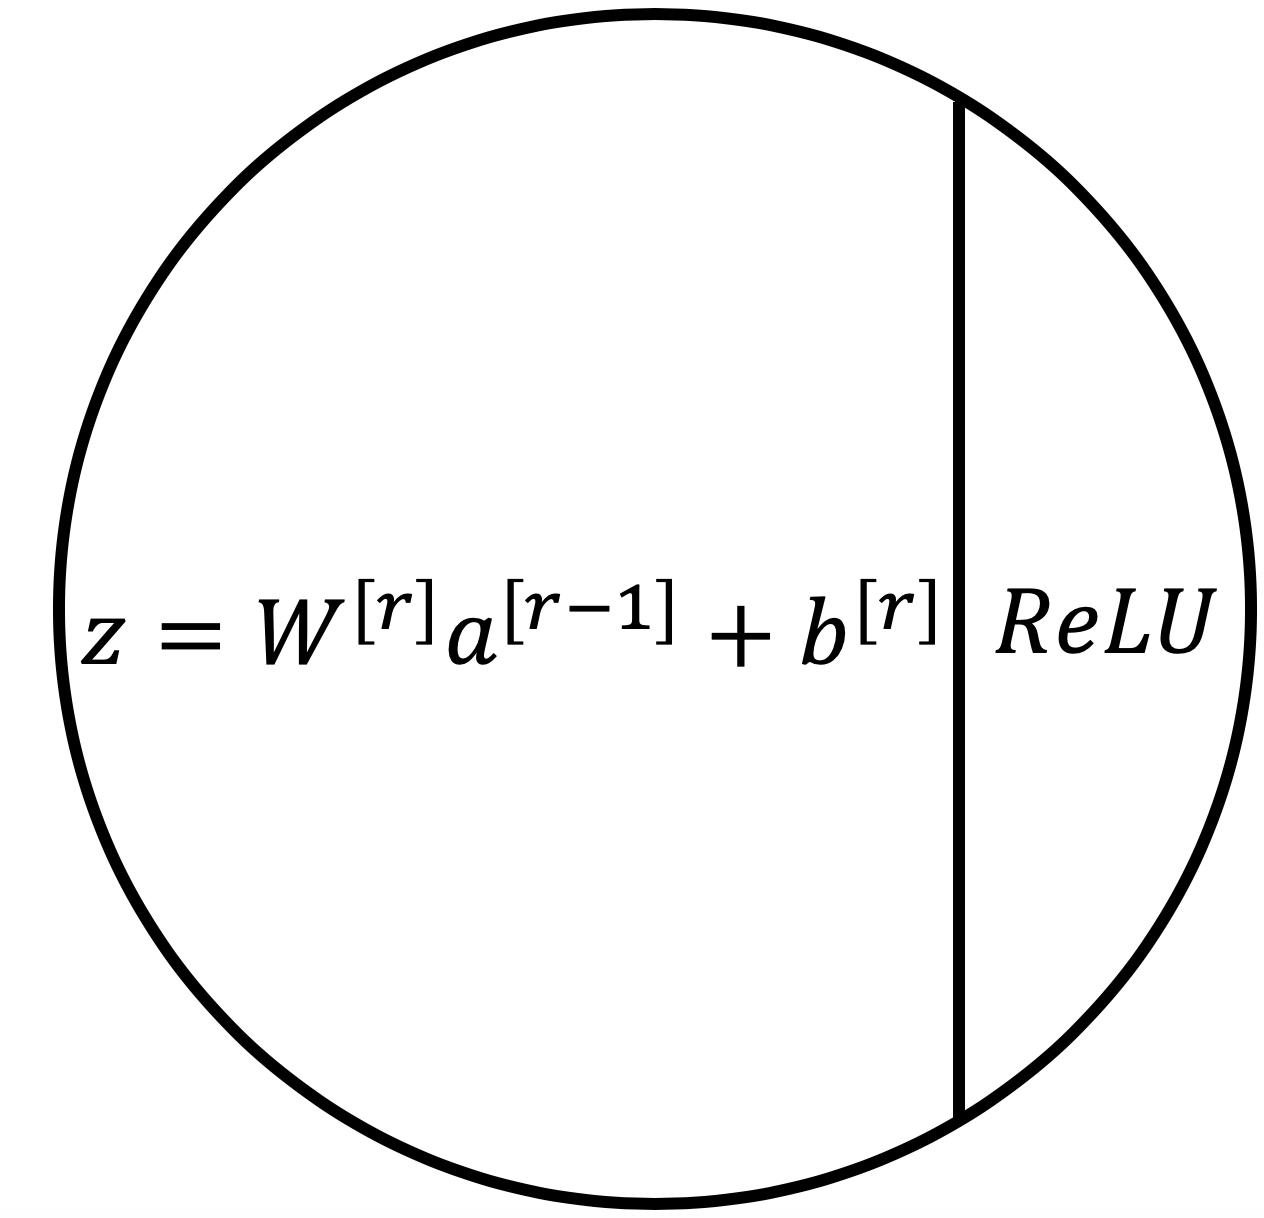
\includegraphics[width=0.3\textwidth]{images/08NNNode.png}
    \caption{Inside a hidden layer's node.}
    \label{fig:08NNNode}
\end{figure}

Mathematically, for one example $x$:
\begin{center}
    $z^{[1]}_j = W^{[1]}x + b^{[1]}$ \\
    $a^{[1]}_j = ReLU(z^{[1]}_j)$ \\
    $z^{[2]}_j = W^{[2]}a^{[1]}_j + b^{[2]}$ \\
    $a^{[2]}_j = ReLU(z^{[2]}_j)$ \\
    ... \\
    $z^{[r]}_j = W^{[r]}a^{[r - 1]}_j + b^{[r]}$ \\
    $a^{[r]}_j = ReLU(z^{[r]}_j)$ \\
    $y = W^{[o]}a^{[r]}_j + b^{[o]}$ \\  
\end{center}

The hyper parameters for each neural network is given in Table \ref{tab:08NN_hp}. $\lambda$ was increased as the neural network got more complex to reduce overfitting.  The ReLU activation function was chosen for computational efficiency and avoiding the exploding/vanishing gradient problem \cite{ReLU}.
\begin{table}[h]
    \centering
    {\setstretch{1.2}
    \begin{tabular}{ c | c | c | c}
        Hyper Parameter                            &  Small NN  &  Med. NN  & Large NN       \\
        \hline
        Epochs                                     &  700       & 1000      & 1200  \\
        Minibatch size                             &  8192      & 8192      & 8192  \\
        Learning rate, $\alpha$                    &  0.001     & 0.001     & 0.001 \\
        Regularization, $\lambda$                  &  0.001     & 0.003     & 0.005 \\
        Number of layers                           &  3         & 6         & 8     \\
        Neurons per layer                          &  20        & 30        & 40    \\
        Activation function for hidden layers      & ReLU       & ReLU      & ReLU  \\
    \end{tabular}}
    \caption{Hyper parameters for the feed-forward neural network.}
    \label{tab:08NN_hp}
\end{table}

Table \ref{tab:08_nn} shows the performance assessment of the small, medium and large neural networks.  In all cases, the training and validation data set performance was significantly better compared to the linear model; however, the performance was only slightly better on the test data set. On the training and validation data, the error went down by up to 61\%.  On the test data, error went down by up to 19\%. The difference may be caused by the test data being different from the training data.  Due to the complexity of neural network models, they perform exceptionally well on data that shares similar characteristics as the training data, but perform poorly otherwise. To close the gap in performance, a higher $\lambda$ could be used to reduce model complexity.  Moreover, smaller neural networks could also be explored to reduce model complexity.

\begin{table}[h]
\centering
{\setstretch{1.2}
\begin{tabular}{c|c|c|c|c|c|c|c|c|c|}
\multicolumn{1}{l|}{} & \multicolumn{3}{c|}{Training Data}                                               & \multicolumn{3}{c|}{Validation Data}                                             & \multicolumn{3}{c|}{Test Data}                                                   \\ \cline{2-10} 
\multicolumn{1}{l|}{} & \multicolumn{1}{c|}{Sm.} & \multicolumn{1}{c|}{Med.} & \multicolumn{1}{c|}{Lar.} & \multicolumn{1}{c|}{Sm.} & \multicolumn{1}{c|}{Med.} & \multicolumn{1}{c|}{Lar.} & \multicolumn{1}{c|}{Sm.} & \multicolumn{1}{c|}{Med.} & \multicolumn{1}{c|}{Lar.} \\ \hline
MAE                   & 48                       & 42                        & 38                        & 50                       & 45                        & 37                        & 87                       & 87                        & 91                        \\
RMSE                  & 66                       & 58                        & 57                        & 69                       & 61                        & 56                        & 117                      & 107                       & 118                       \\
\end{tabular}}
    \caption{Performance assessment of the neural network models.}
    \label{tab:08_nn}
\end{table}

The comparison of actual and predicted flow rates on the validation and test data for the neural nets are shown in Figures \ref{fig:08smallnn_valid} to \ref{fig:08largenn_test}.  

\begin{figure}[p]
     \centering
     \begin{subfigure}[b]{0.48\textwidth}
         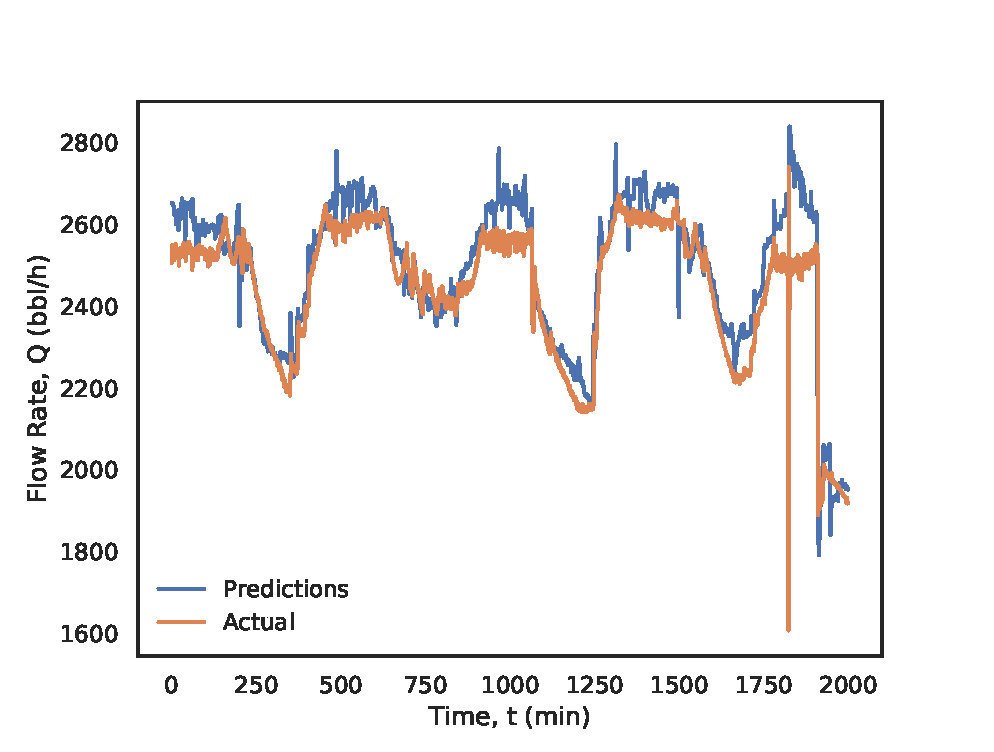
\includegraphics[width=\textwidth]{images/08smallnn_valid.eps}
         \caption{Predicted vs. actual flow rate for validation data using the small neural net.}
         \label{fig:08smallnn_valid}
     \end{subfigure}
     \begin{subfigure}[b]{0.48\textwidth}
         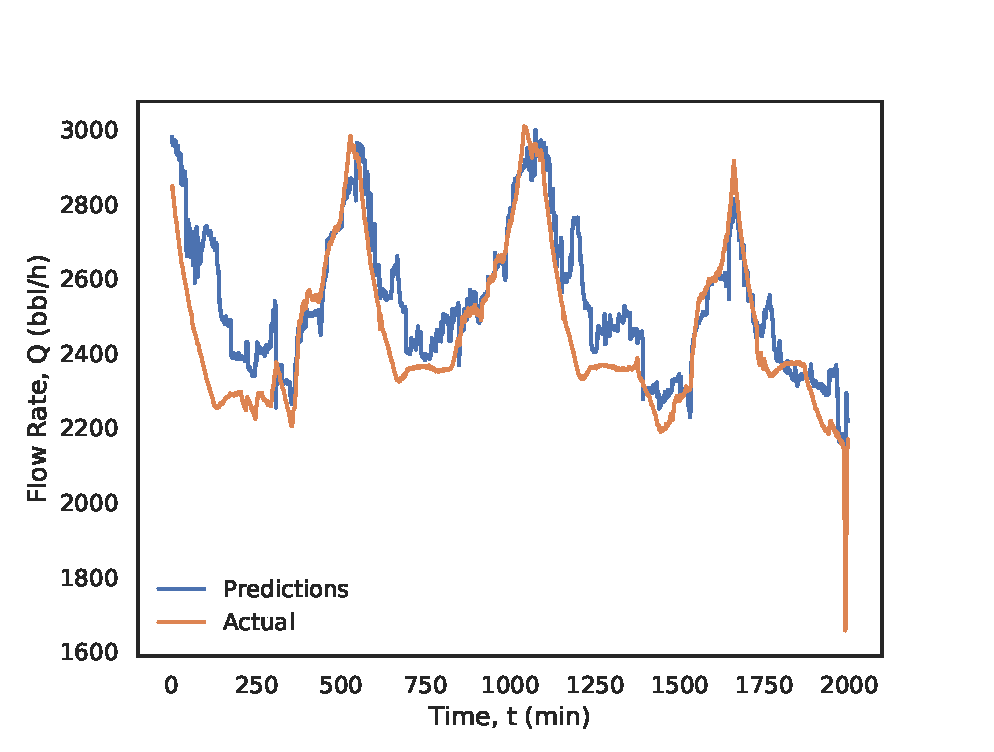
\includegraphics[width=\textwidth]{images/08smallnn_test.eps}
         \caption{Predicted vs. actual flow rate for the test data using the small neural net.}
         \label{fig:08smallnn_test}
     \end{subfigure}
     \begin{subfigure}[b]{0.48\textwidth}
         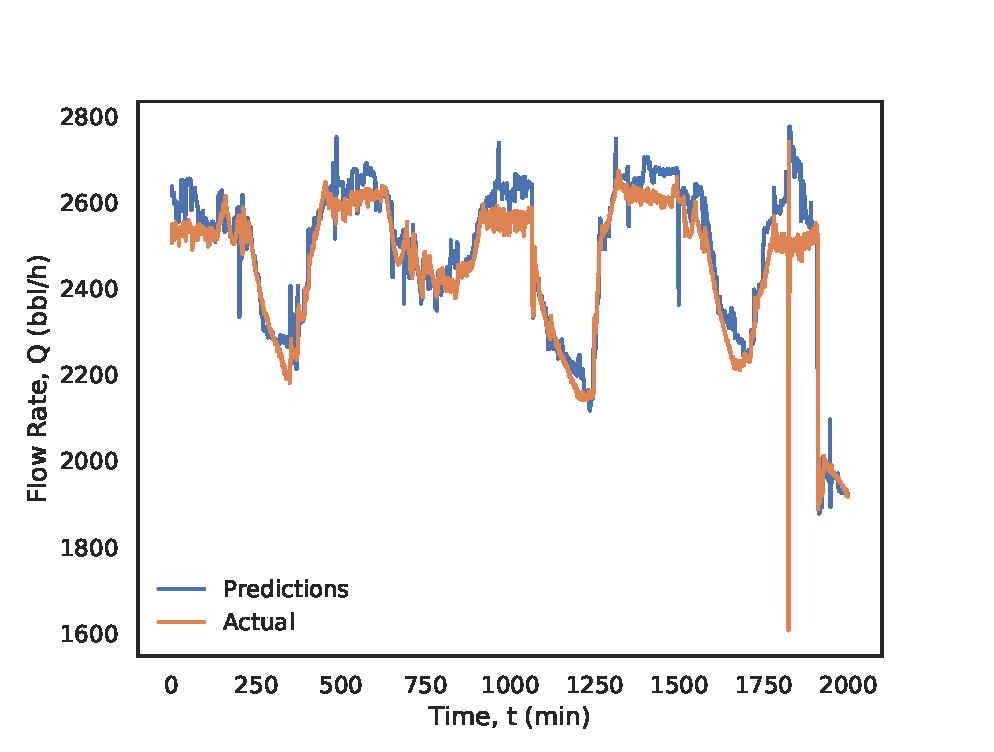
\includegraphics[width=\textwidth]{images/08mednn_valid.eps}
         \caption{Predicted vs. actual flow rate for the validation data using the med. neural net.}
         \label{fig:08mednn_valid}
     \end{subfigure}
     \begin{subfigure}[b]{0.48\textwidth}
         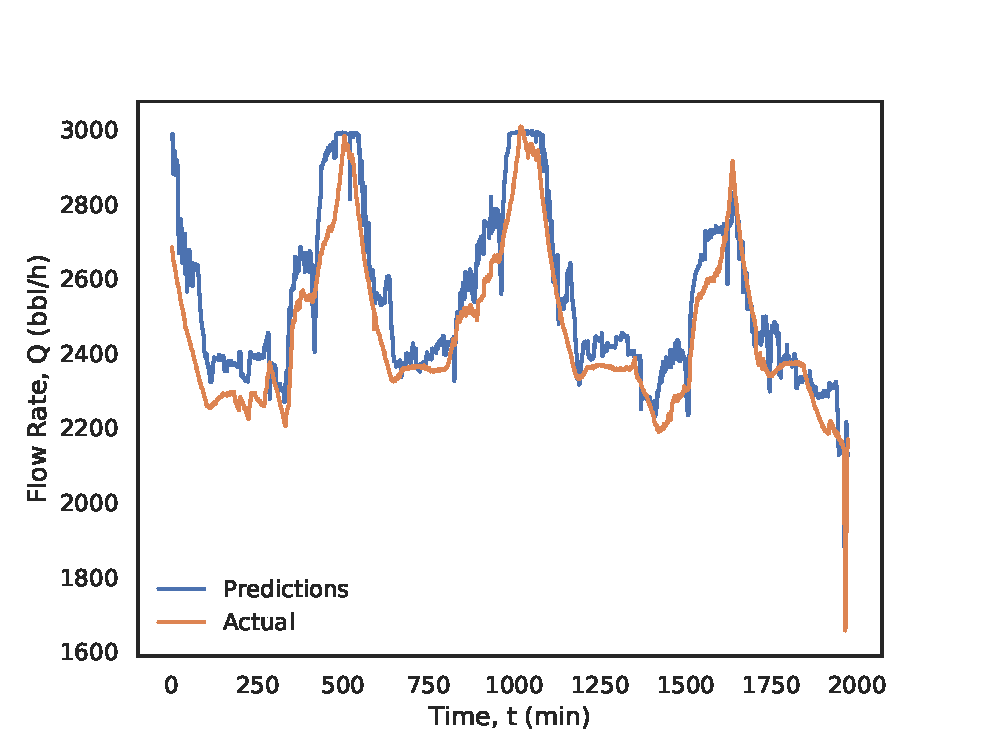
\includegraphics[width=\textwidth]{images/08mednn_test.eps}
         \caption{Predicted vs. actual flow rate for the test data using the med. neural net.}
         \label{fig:08mednn_test}
     \end{subfigure}
     \begin{subfigure}[b]{0.48\textwidth}
         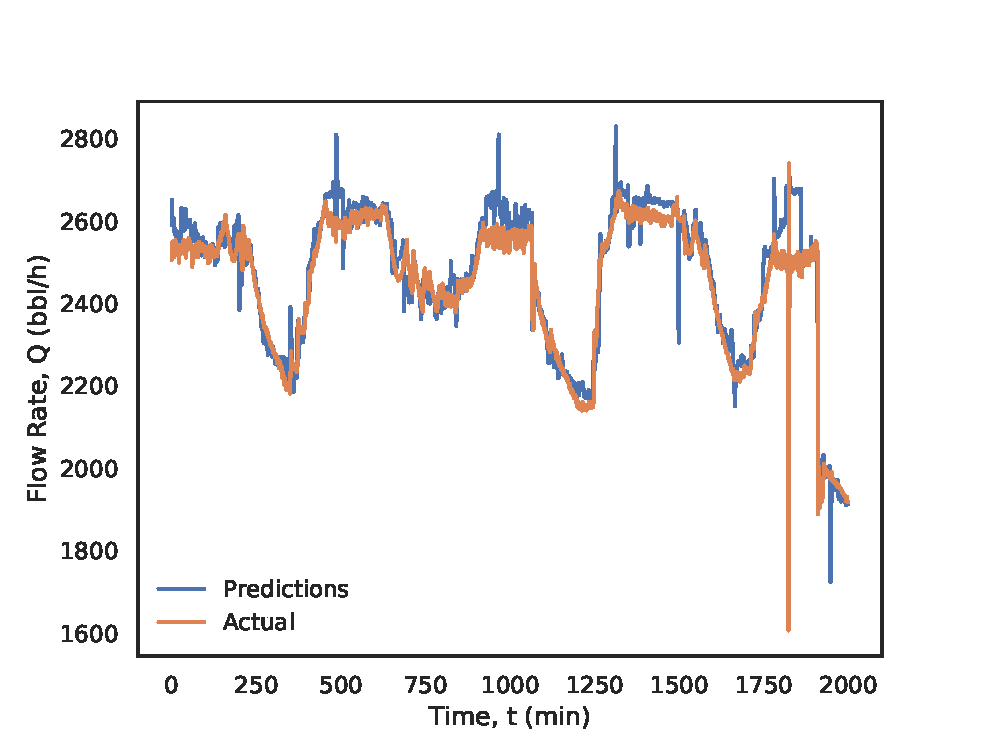
\includegraphics[width=\textwidth]{images/08largenn_valid.eps}
         \caption{Predicted vs. actual flow rate for the validation data using the large neural net.}
         \label{fig:08largenn_valid}
     \end{subfigure}
     \begin{subfigure}[b]{0.48\textwidth}
         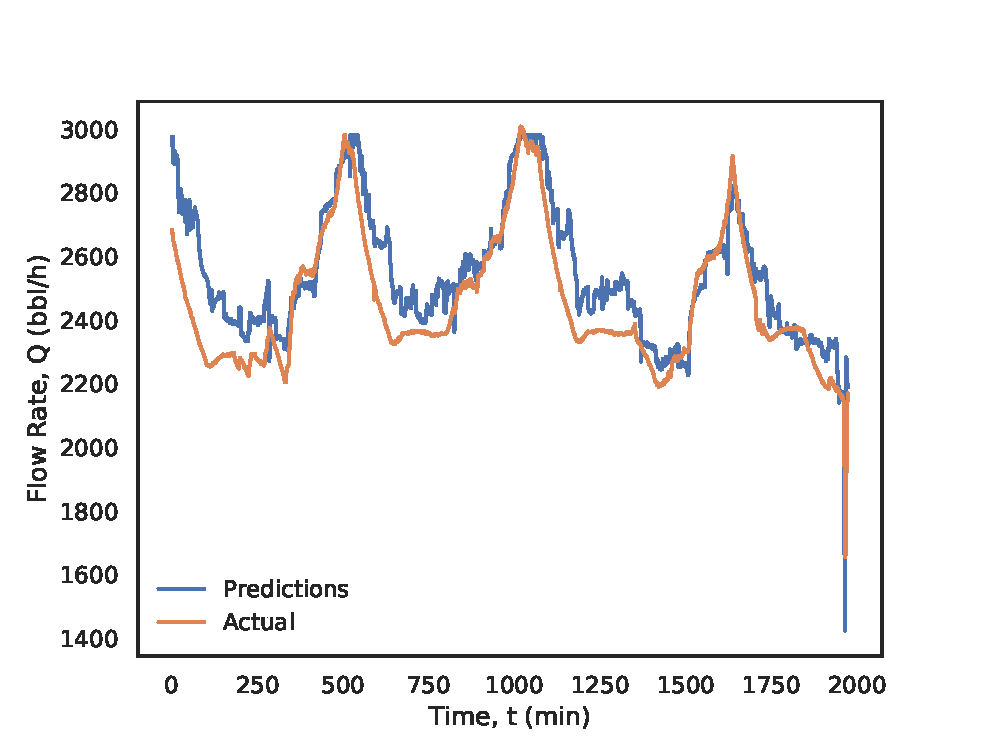
\includegraphics[width=\textwidth]{images/08largenn_test.eps}
         \caption{Predicted vs. actual flow rate for the test data using the large neural net.}
         \label{fig:08largenn_test}
     \end{subfigure}
        \caption{Feed-forward neural network validation and test plots.}
        \label{fig:08PolynomialPlots}
\end{figure}

%%%%%%%%%%%%%%%%%%%%%%%%%%%%%%%%%%%%%%%%%%%%%%%%%%%%%%%%%%%%%%%%%%%%%
%
% LPV MODELS
%
%%%%%%%%%%%%%%%%%%%%%%%%%%%%%%%%%%%%%%%%%%%%%%%%%%%%%%%%%%%%%%%%%%%%%
\noindent
\textit{Linear Parameter-varying Models} \\
Lastly, the linear parameter-varying model (LPV) was explored to model the pipeline. It is clear that the process is non-linear due to the increase in accuracy when switching to a non-linear model structure. LPV models were selected due to their non-linear nature while still retaining the interpretability of linear models. Furthermore, any non-linear model can be approximated by a set of linear models \cite{LPV}. The LPV model is given by:
\begin{equation}
    \begin{split}
        \hat{y} = W_{1, 1}^Tx + W_{1, 2}^Tu + b_1 \\
        \hat{y} = W_{2, 1}^Tx + W_{2, 2}^Tu+ b_2 \\
        ... \\
        \hat{y} = W_{n, 1}^Tx + W_{n, 2}^Tu + b_n \\
    \end{split}
    \label{eq:08LPV_structure}
\end{equation}
where $n \geq 1$ represents the number of linear models used to capture the data set. Here, $W_n$ and $b_n$ are the weights and biases corresponding to the $n^{th}$ model, respectively. For this study, $n=2$.  The models corresponded to the two clusters identified in Figure \ref{fig:08DBSCAN}.  Models 1 and 2 are identified from clusters 1 and 2, respectively.  The hyper parameters for models 1 and 2 are identical to the previous linear models, and are shown in Table \ref{tab:08LSHparameters}. During online implementation, the model will be selected based on the Euclidean distance between the features of the new data and the centroid of the two clusters.  However, if the distance exceeds 1.15 in both cases, the data will be labeled as anomalous.

The performance assessment of the two LPV models are shown in Table \ref{tab:08cluster1_cluster2_reg}. Overall, the LPV models were able to reduce modelling error compared to normal linear regression. Model 1 was only used to predict high flow rate scenarios. Nevertheless, its MAE and RMSE were still 8\% lower compared to the linear regression model used to predict for all data.  For model 2, the MAE and RMSE were up to 31\% lower. 

\begin{table}[h]
    \centering
    {\setstretch{1.2}
    \begin{tabular}{c|c|c|c|c|c|c|}
      & \multicolumn{2}{c|}{Training data} & \multicolumn{2}{c|}{Validation data} & \multicolumn{2}{c|}{Test data} \\ \cline{2-7} 
      & Cl. 1            & Cl. 2           & Cl. 1             & Cl. 2            & Cl. 1          & Cl. 2         \\ \hline
    MAE   & 90               & 66              & 90                & 67               & 96             & 85            \\
    RMSE  & 115              & 91              & 116               & 92               & 120            & 110           \\
    $R^2$ & 0.87             & 0.90            & 0.86              & 0.89             & 0.78           & 0.57         
    \end{tabular}}
    \caption{Performance assessment for clusters 1 and 2 regression models.}
    \label{tab:08cluster1_cluster2_reg}
\end{table}

The comparison of actual and predicted flow rates on the validation and test data for the LPV models are shown in Figures \ref{fig:08cluster1_valid} to \ref{fig:08cluster2_test}. In Figures \ref{cluster2_valid} and \ref{cluster2_test}, it can be seen that model 2 performs poorly on the data.  This might be caused by some unobserved variables that are only applicable for low flow rate operations.
\begin{figure}[h]
    \centering
     \begin{subfigure}[b]{0.48\textwidth}
         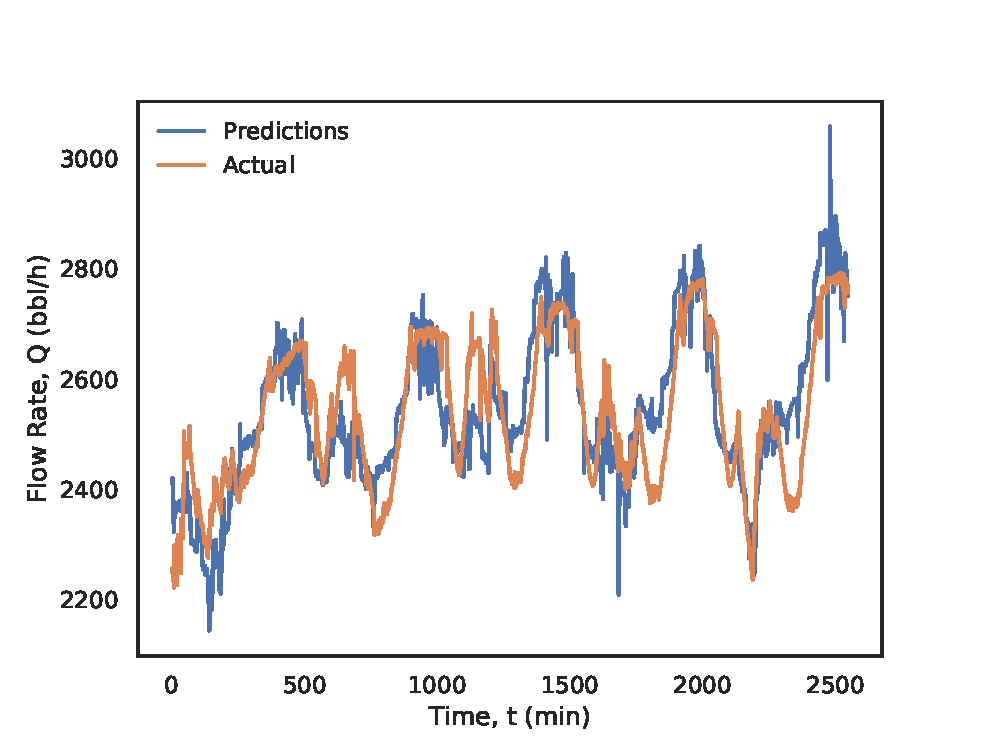
\includegraphics[width=\textwidth]{images/08cluster1_valid.eps}
         \caption{Predicted vs. actual flow rate for validation data using model 1.}
         \label{fig:08cluster1_valid}
     \end{subfigure}
     \begin{subfigure}[b]{0.48\textwidth}
         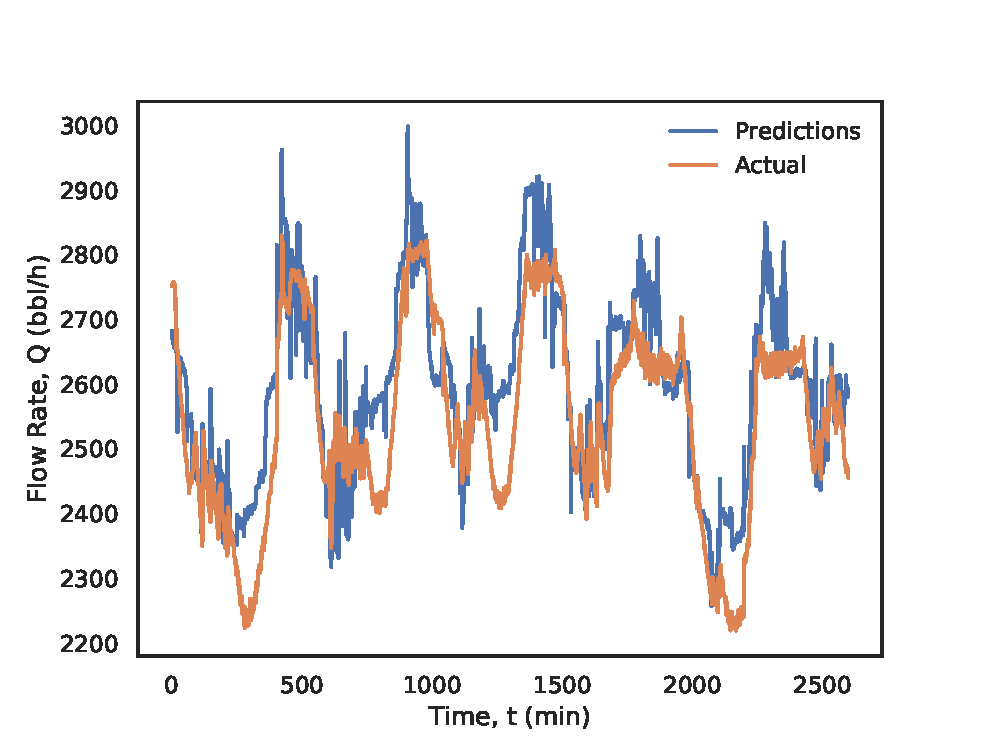
\includegraphics[width=\textwidth]{images/08cluster1_test.eps}
         \caption{Predicted vs. actual flow rate for the test data using model 1.}
         \label{fig:08cluster1_test}
     \end{subfigure}
     \begin{subfigure}[b]{0.48\textwidth}
         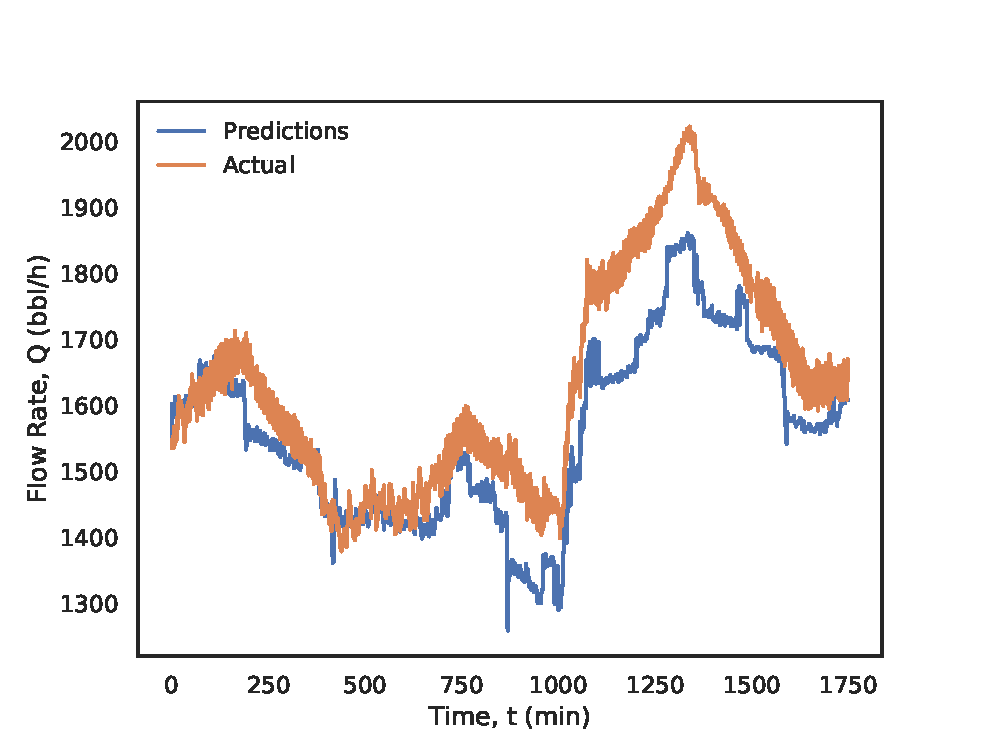
\includegraphics[width=\textwidth]{images/08cluster2_valid.eps}
         \caption{Predicted vs. actual flow rate for the validation data using model 2.}
         \label{fig:08cluster2_valid}
     \end{subfigure}
     \begin{subfigure}[b]{0.48\textwidth}
         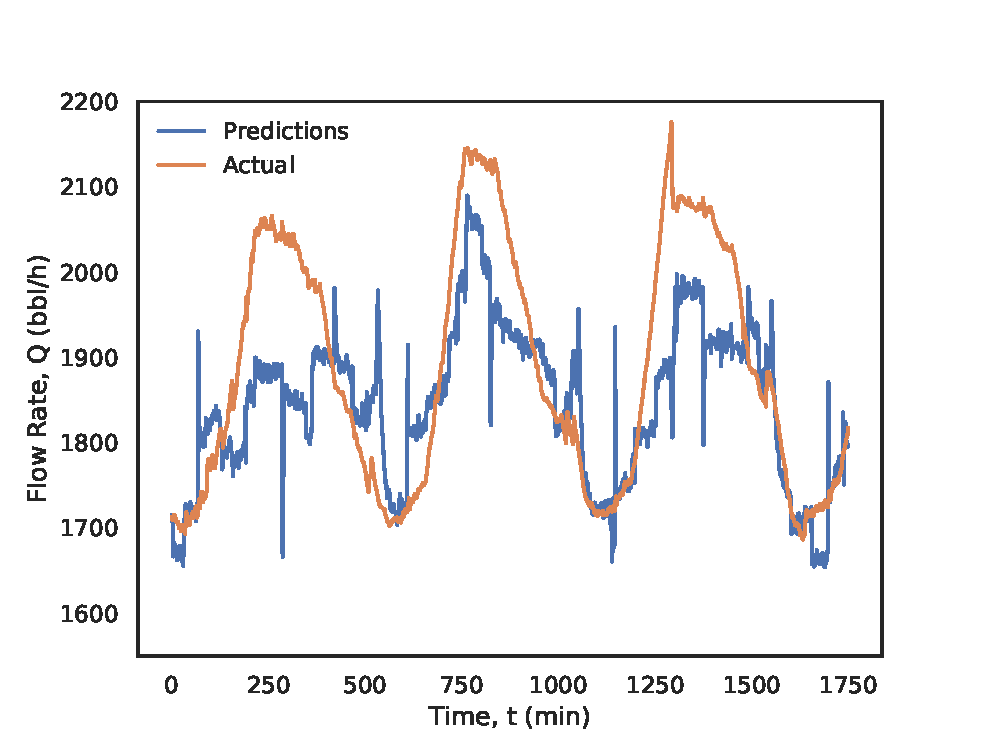
\includegraphics[width=\textwidth]{images/08cluster2_test.eps}
         \caption{Predicted vs. actual flow rate for the test data using model 2.}
         \label{fig:08cluster2_test}
     \end{subfigure}
        \caption{Linear parameter-varying models' validation and test plots.}
        \label{fig:08PolynomialPlots}
\end{figure}

Ultimately, the LPV model structure was selected to model the pipeline.  The LPV model has the interpretability of linear models, while having the predictive capabilities of non-linear models.  Furthermore, the LPV model identifies a separate set of parameters for the two distributions, making the optimization algorithm more representative of live operations.  For example, because no DRA was used for lower flow rates, the optimization algorithm will have explicit constraints on model 2 to not use DRA as well. A similar example would be using only Ault booster 1 for cluster 2, while using Ault booster 2 for cluster 1.  The advantages of these constraints are twofold: i) More realistic to live operations.  ii) Avoid model extrapolations (since no DRA data was used to identify model 2, the optimizer should not be able to use it for optimization).

\subsubsection{Time-series Modelling}
All previous models are static (i.e., $y_{ss} = f(x, u)$) and are used for the real time optimization layer in Figure \ref{fig:08APC}. To completely automate the pipeline operations, a dynamic model was identified for the application of supervisory control. In dynamic modelling, temporal correlations within the time-series data are exploited to improve model accuracy.  Moreover, $y_t$ is measured at each time and can be used to further improve model accuracy. The time-series model will have the following structure:
\begin{equation}
    y_{t+1} = f(x_{t}, x_{t - 1}, ..., x_{t-p}, u_{t}, u_{t - 1}, ..., u_{t - q}, y_{r})
\end{equation}
Here, subscripts $p$ and $q$ denote the number of previous states and inputs to be considered in the model, respectively.  Subscript $r = max(p, q)$. Least squares will be used to identify the time-series model with data augmented as $[x_t, u_t | x_{t - 1}, u_{t - 1} | ... ]$.  After exploring a variety of $p$'s and $q$'s, the final hyper parameters used for the time series model is shown in Table \ref{tab:08ts_parameters}.
\begin{table}[h]
    \centering
    {\setstretch{1.2}
    \begin{tabular}{ c | c}
        Hyper Parameter                  &  Value       \\
        \hline
        Epochs                           &  1000      \\
        Minibatch size                   &  8192     \\
        Learning rate, $\alpha$          &  0.001    \\
        Regularization, $\lambda$        &  0.001    \\
        $\#$ of previous states, $p$     &  2  \\
        $\#$ of previous inputs, $q$     &  2  \\
    \end{tabular}}
    \caption{Hyper parameters for the time-series least squares model.}
    \label{tab:08ts_parameters}
\end{table}

The performance metrics of the time-series model is shown in Table \ref{tab:08ts_performance}.  Compared to static models, dynamic models are significantly more accurate; error metrics went down by up to 87\%.
\begin{table}[h]
    \centering
    {\setstretch{1.2}
    \begin{tabular}{ c | c | c | c}
                             &  Training data    &  Validation data   &    Test data      \\
        \hline
        MAE                  &      22           &        17          &   25    \\
        RMSE                 &      41           &        34          &   65    \\ 
        $R^2$                &      0.99         &        0.99        &   0.86  \\
    \end{tabular}}
    \caption{Performance assessment for the time-series least squares model.}
    \label{tab:08ts_performance}
\end{table}

The comparison of actual and predicted flow rates on the validation and test data for the time-series least square model are shown in Figure \ref{fig:08ts_ls}. 
\begin{figure}[h]
    \centering
     \begin{subfigure}[b]{0.48\textwidth}
         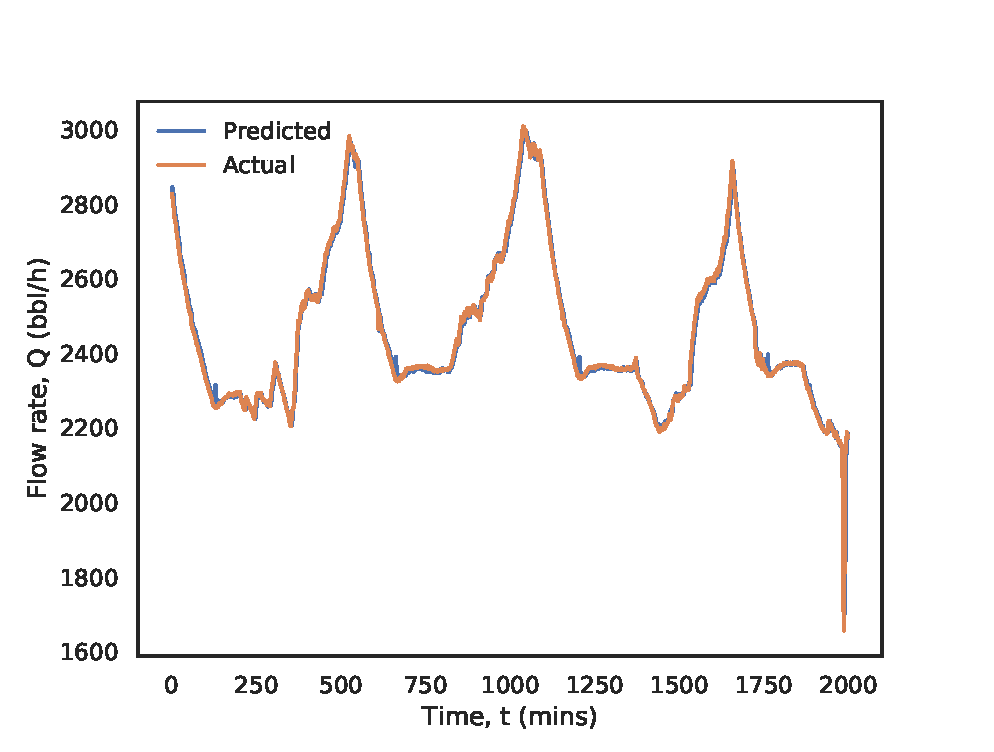
\includegraphics[width=\textwidth]{images/08ts_validation.eps}
         \caption{Validation data.}
         \label{fig:08ts_valid}
     \end{subfigure}
     \begin{subfigure}[b]{0.48\textwidth}
         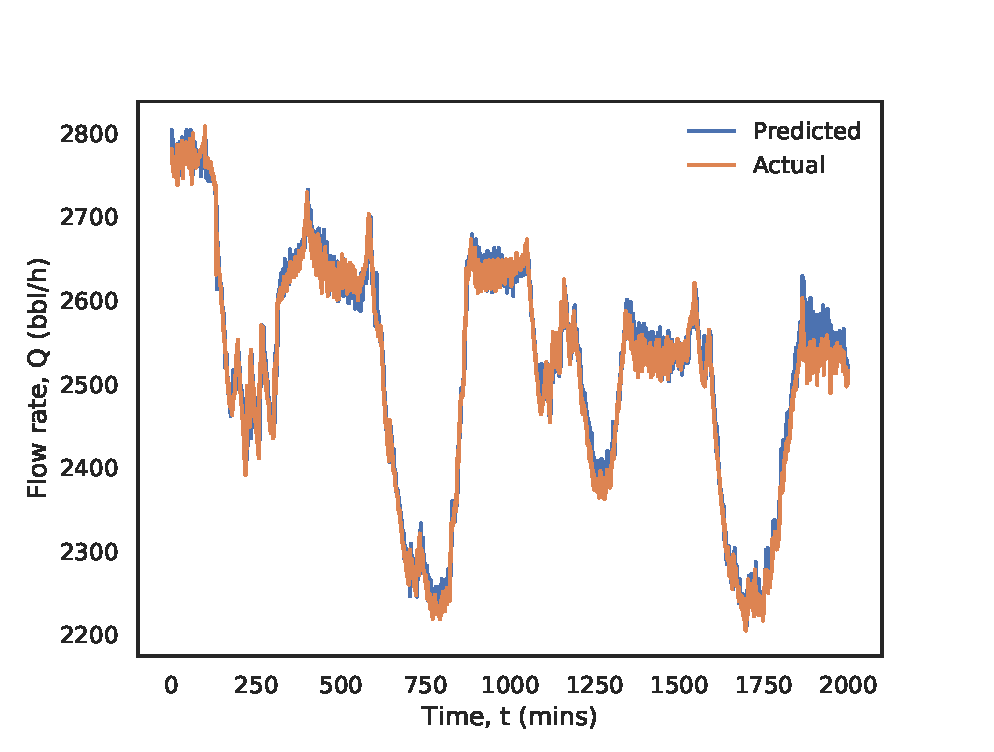
\includegraphics[width=\textwidth]{images/08ts_test.eps}
         \caption{Test data.}
         \label{fig:08ts_test}
     \end{subfigure}
        \caption{Predicted vs. actual flow rate using the time-series model.}
        \label{fig:08ts_ls}
\end{figure}


\subsubsection{Model Applicability Range}
Extrapolation while using data-driven models introduce risks to operations. Thus, Tables \ref{tab:08StateConst} and \ref{tab:08InputConst} show the ranges of states and inputs where the model is most effective. The ranges were identified from $\mu - 2\sigma \leq x, u \leq \mu + 2\sigma$ to ensure the range captures 95.5\% of the data while omitting outliers. Usage of the models beyond the normal range may be ineffective.

\begin{table}[h]
    \centering
    {\setstretch{1.2}
    \begin{tabular}{ p{5cm} | c }
        Variables                         &  Valid Range           \\
        \hline
        Flow Rate (bbl/h)                       &      1765 - 3000       \\
        Cheyenne Density (API)                  &      22 - 47           \\ 
        CIG Density (API)                       &      15 - 45           \\
        Ault Density (API)                      &      15 - 45           \\
        Cheyenne Temp (°C)                      &      35 - 50           \\
        CIG Temp (°C)                           &      41 - 51           \\
        Ault Temp (°C)                          &      43 - 54           \\
        Fort Lupton Temp (°C)                   &      48 - 60           \\
        Commerce City Temp  (°C)                &      40 - 58           \\
    \end{tabular}}
    \caption{Applicable states of the machine learning models.}
    \label{tab:08StateConst}
\end{table}

In addition to the state ranges provided above, the recommended set points are also limited to avoid extrapolation.  The set point ranges are shown in Table \ref{tab:08InputConst}.

\begin{table}[h]
    \centering
    {\setstretch{1.2}
    \begin{tabular}{ p{6cm} | c }
        Variables                               &  Valid Range            \\
        \hline
        Cheyenne VFD (Amps)                     &      105 - 322          \\
        Fort Lupton VFD (Amps)                  &      78 - 134           \\ 
        CIG \& Ault Sweet DRA (ppm)             &      20 - 40            \\
        CIG \& Ault Sour DRA (ppm)              &      20 - 40            \\
    \end{tabular}}
    \caption{Applicable inputs of the machine learning models.}
    \label{tab:08InputConst}
\end{table}

\subsubsection{Adaptive Machine Learning}
\paragraph{Online Learning vs. Incremental Learning}
\paragraph{ART: Adaptive Resonance Theory}
\paragraph{Implementation of Adaptive Machine Learning}

\begin{figure}
    \centering
    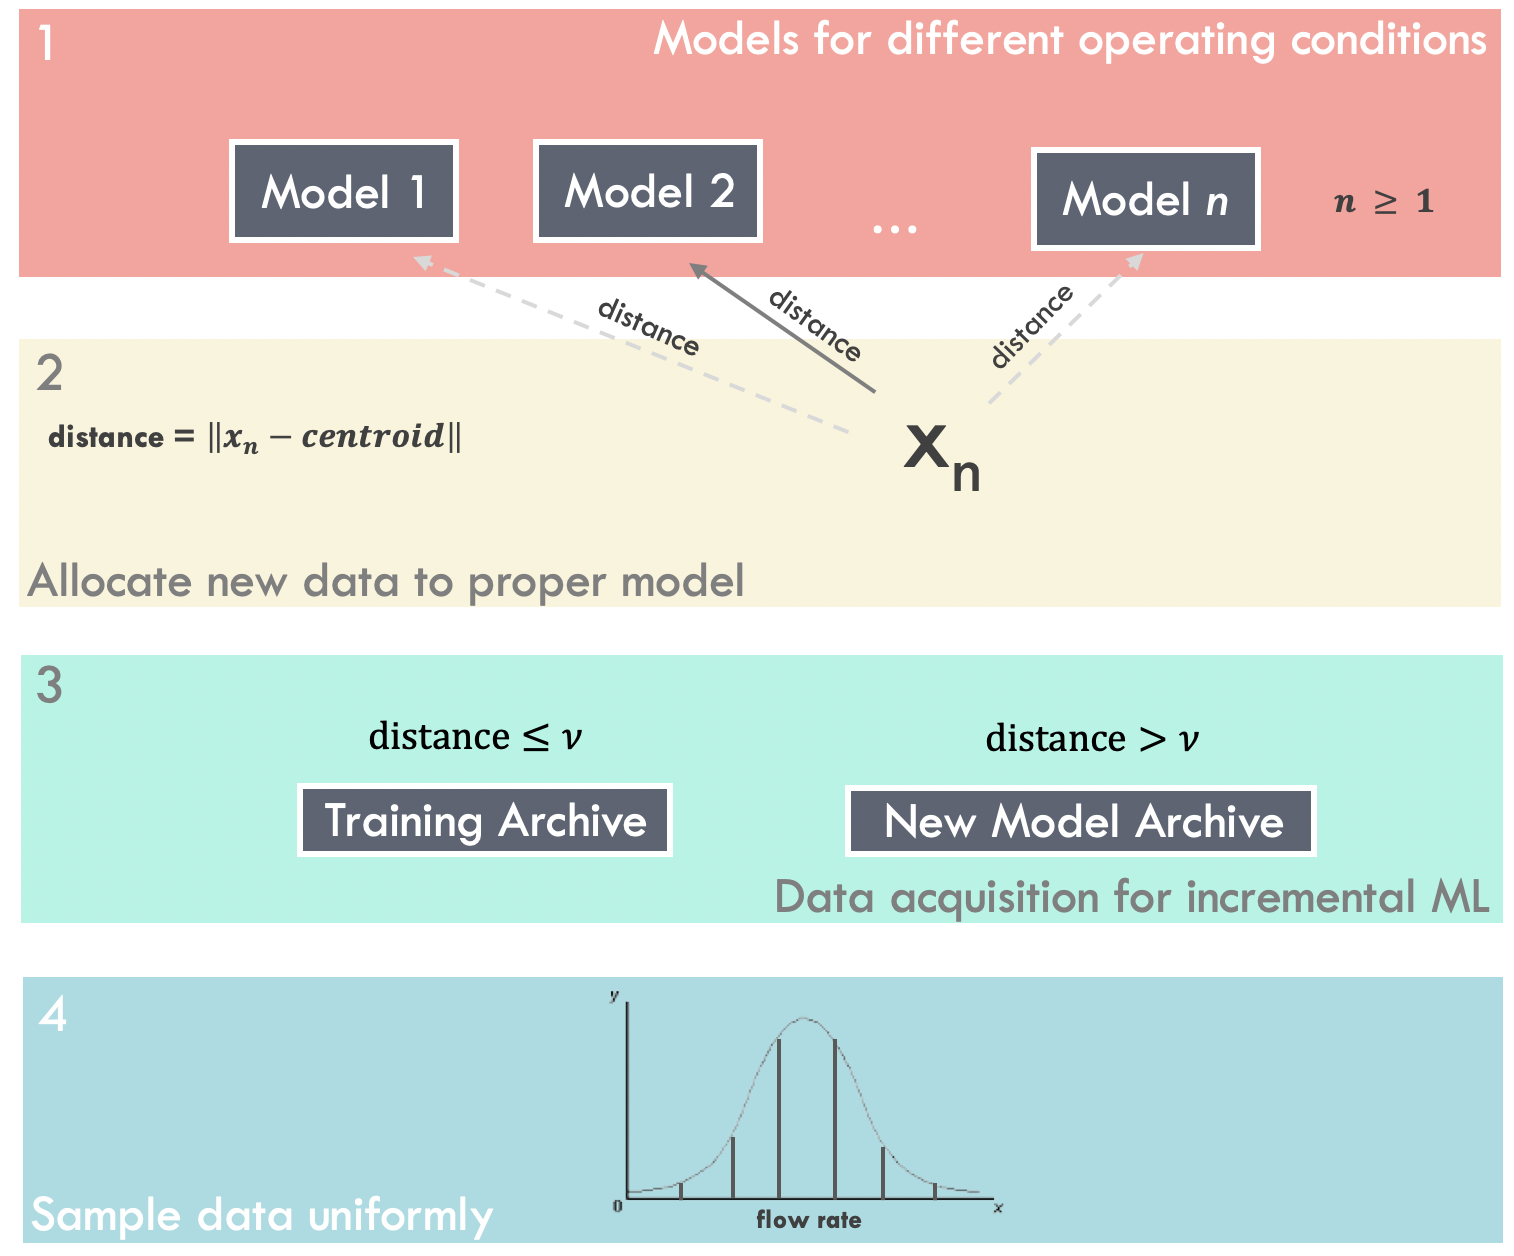
\includegraphics[width=\textwidth]{images/08IncrementalLearning.png}
    \caption{Importance Sampling Incremental Supervised learning architecture.}
    \label{fig:08ART}
\end{figure}

\subsection{Mixed Integer Linear Programming}
The information flow of the optimization algorithm is shown in Figure \ref{fig:08Optimization_flow}.  First, a desired flow will be inputted by the operators depending on the demand from Commerce City.  Then, the machine learning model along with equality and in-equality constraints will be provided to the mixed integer linear program (MILP).  Given the objective function, decision variables, and the current costs, the MILP will finally output the optimal set points.
\begin{figure}[h]
    \centering
    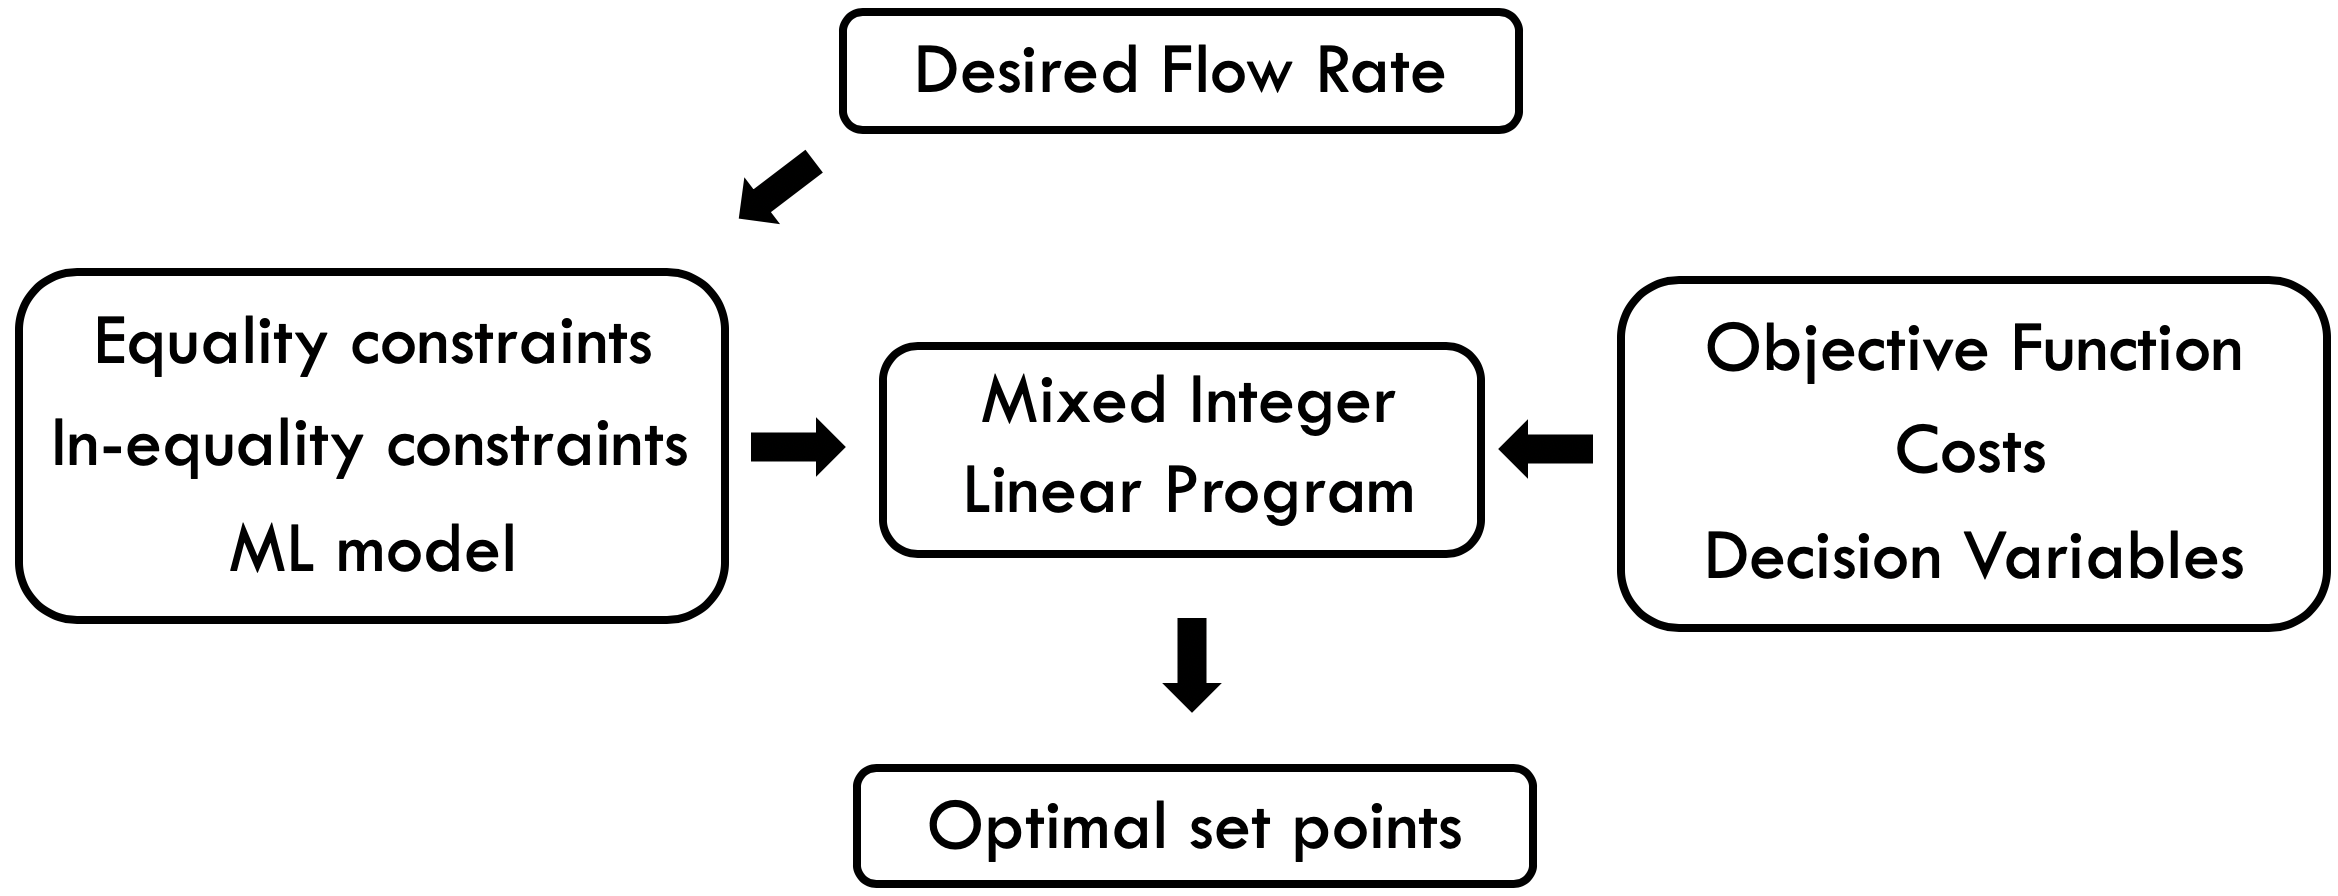
\includegraphics[width=\textwidth]{images/08Optimization_flow.png}
    \caption{Optimization information flow chart.}
    \label{fig:08Optimization_flow}
\end{figure}

\noindent
\textit{Mixed Integer Linear Program} \\
MILP was used to perform steady state optimization on the linear model because the decision variables included binary and continuous variables.  In total, there was 10 decision variables; 4 binary and 6 continuous.  The binary and continuous variables are shown in Table \ref{tab:08binary_cont}.

\begin{table}[h]
    \centering
    {\setstretch{1.2}
    \begin{tabular}{ c | c }
        Binary                       &  Continuous           \\
        \hline
        On/off Cheyenne Pump               &  Cheyenne \& Fort Lupton VFD            \\
        2$\times$ On/off Ault Pump         &  2$\times$ Sweet \& 2$\times$ Sour DRA  \\
        On/off Fort Lupton Pump
    \end{tabular}}
    \caption{Binary and continuous decision variables.}
    \label{tab:08binary_cont}
\end{table}

\noindent
\textit{Constraints} \\
The constraints are the machine learning model, equality, and in-equality constraints.  The equality and in-equality constraints are shown in Table \ref{tab:08eq_neq_constraints}. From the data provided, the Cheyenne pump was on 95\% of the time, and at least one Ault on/off pump was always on. Therefore, constraints were incorporated to reflect this.  Additionally, constraints were used to ensure proper DRA was injected into the pipeline for the different crudes.  There were also pressure constraints on the outlet pressure of the pumps to ensure safe operations.  Before a recommendation is made to the operators, the set points are used to predict for the outlet pressures at each pump to ensure they do not exceed the maximum allowable working pressure (MAWP). Finally, the flow rate is given a range to ensure optimization feasibility. Specifying exact flow rates lead to infeasible solutions because there may not exist a combination to get an \textit{exact} flow rate.

\begin{table}[h]
    \centering
    {\setstretch{1.5}
    \begin{tabular}{c|c}
         Equality Constraints              & In-equality Constraints \\
         \hline
         On/off Cheyenne Pump = On         & $\text{Lower bound} \leq \text{Flow rate} \leq \text{Upper bound}$ \\
         
         Ault Pump 1 and/or 2 = On          & $P_{Outlet}^{Chey} \leq 1480 \text{ psi}$       \\
         
         $API^{CIG} \geq 30: DRA_{Sweet}^{CIG}$ = On & $P_{Outlet}^{Ault} \leq 1613 \text{ psi}$ \\
         
         $API^{CIG} \leq 30: DRA_{Sour}^{CIG}$ = On  & $P_{Outlet}^{FL} \leq 1613 \text{ psi}$  \\
         
         $API^{Ault} \geq 30: DRA_{Sweet}^{Ault}$ = On & $20 \text{ ppm} \leq DRA \leq 40 \text{ ppm}$                 \\
         
         $API^{Ault} \leq 30: DRA_{Sour}^{Ault}$  = On  & $105 \text{ Amps} \leq VFD^{Chey} \leq 322 \text{ Amps}$   \\
         
         Cheyenne On/off = 28 Amps  & $78 \text{ Amps} \leq VFD^{FL} \leq 134 \text{ Amps}$  \\
         Ault 1 Pump = 190 Amps & \\
         Ault 2 Pump = 278 Amps & \\
         Fort Lupton Pump = 117 & \\
    \end{tabular}}   
    \caption{List of equality and inequality constraints}
    \label{tab:08eq_neq_constraints}
\end{table}

Pressure models were built to ensure MAWP was not exceeded when the recommended set points are implemented. In the end, three linear regression pressure models were identified; each at the outlet of a pump station (Cheyenne, Ault, Fort Lupton) where pressure is expected to be the highest. The inputs to the pressure models were all upstream of the pump station is located and is given in Table \ref{tab:08pressure_inputs}.

\begin{table}[]
    \centering
    {\setstretch{1.2}
    \begin{tabular}{p{5cm} | p{5cm} | p{5cm}}
         Cheyenne & Ault & Fort Lupton \\
         \hline
         
         Pipeline inlet pressure & Pipeline inlet pressure & Pipeline inlet pressure \\
         
         Cheyenne VFD & Cheyenne VFD & Cheyenne VFD \\
         
         Cheyenne on/off pump & Cheyenne on/off pump & Cheyenne on/off pump \\
         
         Cheyenne temperature & Ault on/off pump 1 & CIG DRA ppm \\
         
         & Ault on/off pump 2 & Ault on/off pump 1 \\
         
         & CIG DRA ppm & Ault on/off pump 2 \\
         
         & Cheyenne temperature & Ault DRA ppm \\
         
         & Ault temperature & Fort Lupton VFD \\
         & & Fort Lupton on/off pump \\
         & & Cheyenne temperature \\
         & & Ault temperature \\
         & & FL temperature \\
    \end{tabular}}
    \caption{Inputs to the pressure constraint models.}
    \label{tab:08pressure_inputs}
\end{table}

The performance assessment of the Cheyenne, Ault, and Fort Lupton pressure constraint models are shown in Table \ref{tab:08pres_const_performance}. The Cheyenne pressure prediction is very accurate; however the accuracy decreases as we traverse down the pipeline.  The primary reason is because an accurate inlet pressure is required to predict for the outlet pressure.  But the inlet pressure beyond Cheyenne is unknown because the set points are not actuated in the pipeline yet. Furthermore, predicting the outlet pressure at Ault is especially difficult because a mechanism exists to limit the pressure to 1377 psi.  The mechanism's data is not captured, and causes the regression curve to be hard constrained at an upper bound. Consequently, this causes many inputs to result in the same output, and hinders learning.

\begin{table}[h]
    \centering
    {\setstretch{1.2}
    \begin{tabular}{c|c|c|c|c|c|c|}
    \multicolumn{1}{l|}{} & \multicolumn{3}{c|}{Training Data} & \multicolumn{3}{c|}{Validation Data} \\ \cline{2-7} 
    \multicolumn{1}{l|}{} & Cheyenne   & Ault   & Fort Lupton  & Cheyenne    & Ault   & Fort Lupton   \\ \hline
    MAE                   & 75         & 179    & 25           & 72          & 179    & 27            \\
    RMSE                  & 101        & 217    & 32           & 96          & 217    & 35            \\
    $R^2$                 & 0.88       & 0.5    & 0.47         & 0.89        & 0.49   & 0.46         
    \end{tabular}}
    \caption{Performance assessment of the Cheyenne, Ault, and Fort Lupton pressure constraint models}
    \label{tab:08pres_const_performance}
\end{table}

The performance of the pressure constraint models on the validation data is shown in Figures \ref{fig:08Chey_Pconst} to \ref{fig:08FL_Pconst}.

\begin{figure}
    \centering
    \begin{subfigure}[b]{0.325\textwidth}
         \centering
         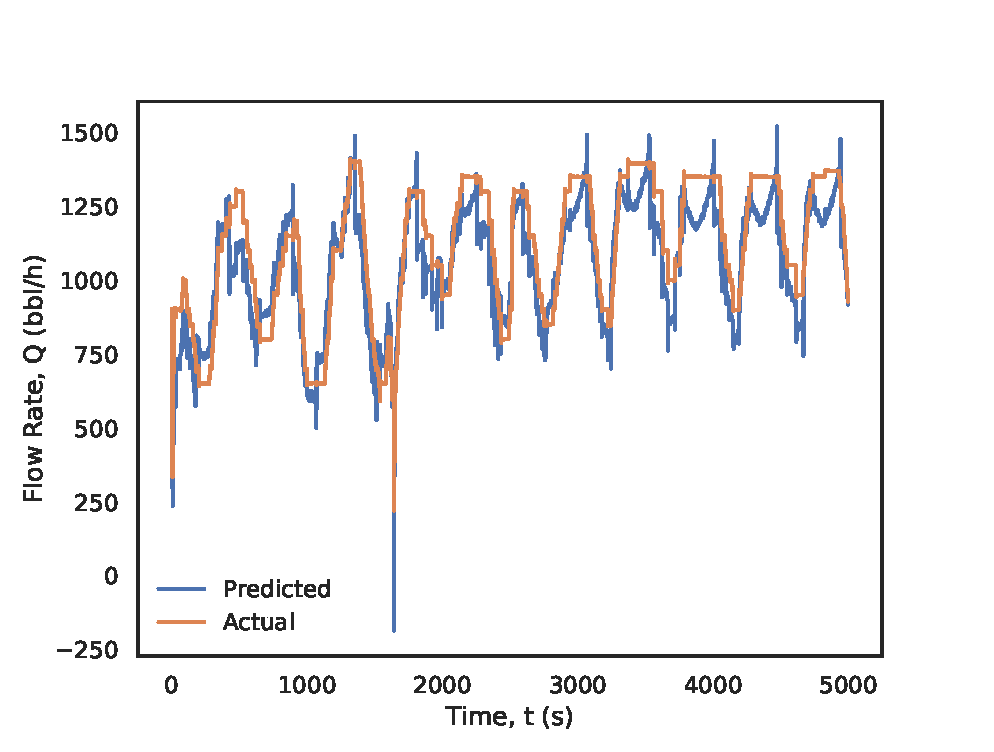
\includegraphics[width=\textwidth]{images/08Chey_Pconst.eps}
         \caption{Cheyenne}
         \label{fig:08Chey_Pconst}
    \end{subfigure}
    \begin{subfigure}[b]{0.325\textwidth}
         \centering
         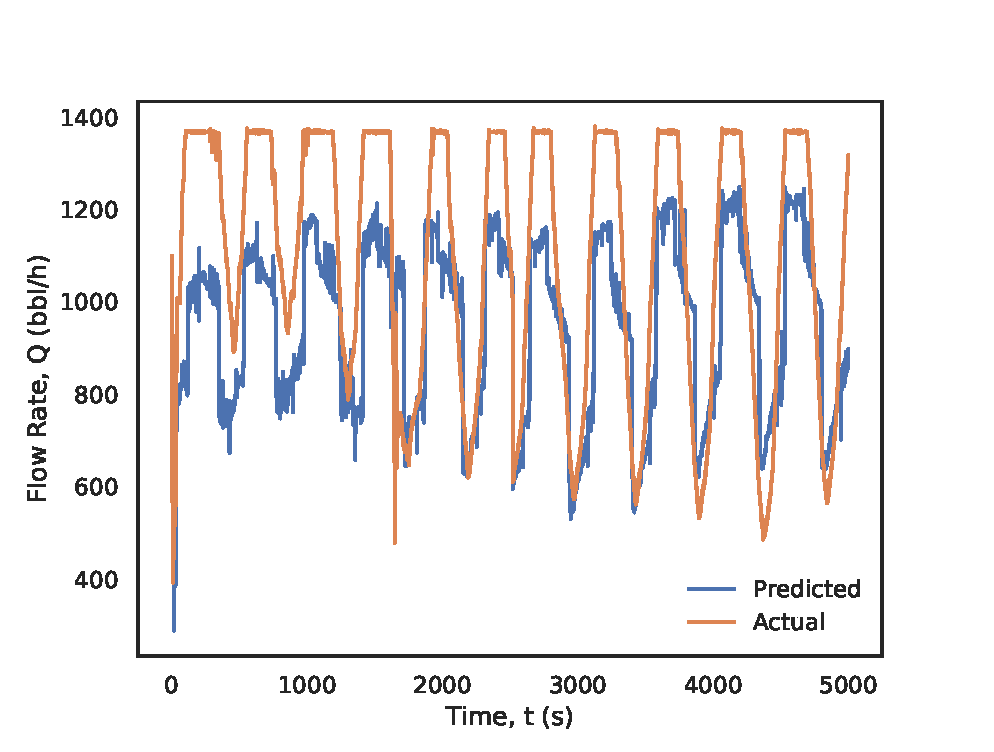
\includegraphics[width=\textwidth]{images/08Ault_Pconst.eps}
         \caption{Ault}
         \label{fig:08Ault_Pconst}
    \end{subfigure}
    \begin{subfigure}[b]{0.325\textwidth}
         \centering
         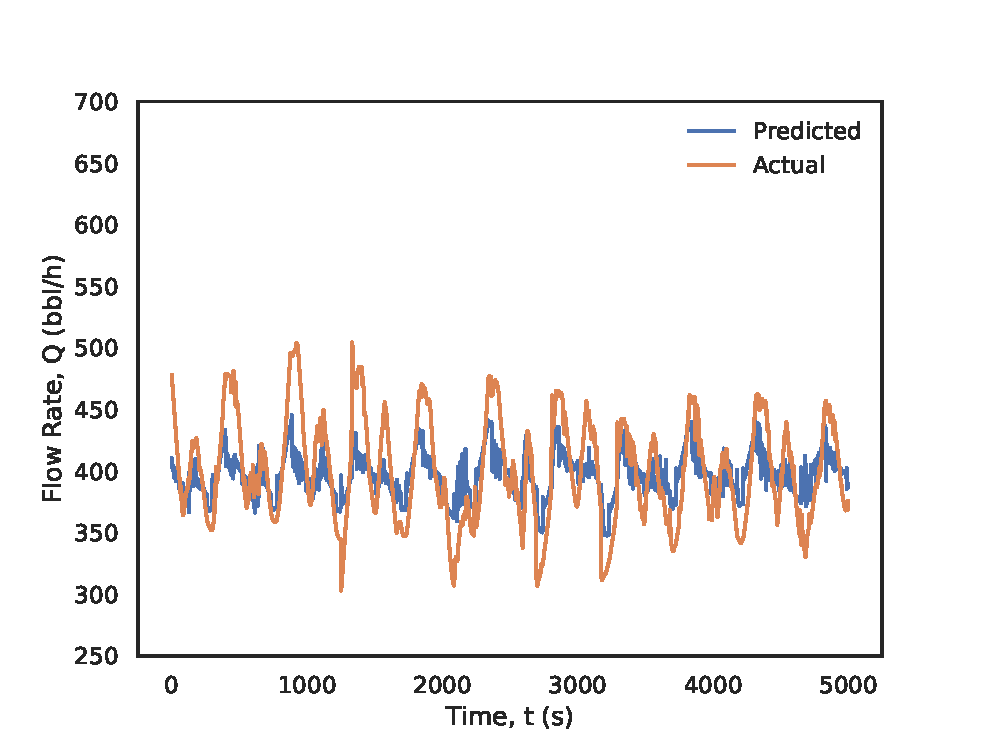
\includegraphics[width=\textwidth]{images/08FL_Pconst.eps}
         \caption{Fort Lupton}
         \label{fig:08FL_Pconst}
    \end{subfigure}
    \caption{Pressure constraint model performance on validation data.}
    \label{fig:08Pconst}
\end{figure}

\noindent
\textit{Objective Function, Costs and Decision Variables} \\
The objective is to operate the pipeline at the desired flow rate with the minimum possible operating cost.  The optimization is given by:

\begin{mini*}|s|
    {J} {= \left[ \alpha_i \sum_i \mu_i \cdot DRA_i + \beta \sum_j \nu_j \cdot I_jV_j \right]}
    {}{}
    \addConstraint{y = f(x, u)}                
    \addConstraint{\nu_{Ault1} + \nu_{Ault2} \geq 1} 
    \addConstraint{\nu_{Chey} = 1} 
    \addConstraint{20 \leq DRA_i \leq 40, \; i \in I} 
    \addConstraint{\gamma_j^{min} \leq I_j \leq \gamma_j^{max}, \; j \in J}{}
\end{mini*}
where $\alpha$ denotes the cost of DRA per ppm, $\beta$ denotes the cost of one kWh, $mu$ denotes the on/off status of the DRA pumps, and $\nu$ denotes the on/off status of the pumps. $DRA_i$ is the DRA ppm set point of the $i^{th}$ DRA injection pump. Moreover, $V_j$ and $I_j$ are the voltage and drawn amperes corresponding to the $j^{th}$ pump. Here, $\gamma_j$ are the upper and lower bounds of the VFDs' currents and are provided in Table \ref{tab:08eq_neq_constraints}. For on/off pumps, $\gamma_j$ is fixed.

The voltages of the pumps are provided in Table \ref{tab:08Voltages}.  The power cost per kWh for the pipeline was \$0.09 USD.
\begin{table}[h]
    \centering
    {\setstretch{1.2}
    \begin{tabular}{c|c}
        Pump          &  Voltage \\
        \hline
        $VFD^{Chey}$    &  4160    \\
        $VFD^{FL}$      &  4160    \\
        On/off $Pump^{Chey}$    & 480   \\
        On/off $Pump^{Ault1}$   & 4000  \\
        On/off $Pump^{Ault2}$   & 4000  \\
        On/off $Pump^{FL}$      & 480   \\
    \end{tabular}}
    \caption{Voltages for the pumps.}
    \label{tab:08Voltages}
\end{table}

The cost to increase DRA ppm is dependent on the flow rate of the pipeline. Higher flow rates require more DRA to be injected; hence a higher cost.  The cost curves for DRA is shown in Figures \ref{fig:08DRA_Cost}.  Given a flow rate, the cost to increase the DRA ppm is given by Equations \ref{eq:08sweet_dra} and \ref{eq:08sour_dra} for the sweet and sour DRA, respectively.

\begin{figure}[h]
    \centering
    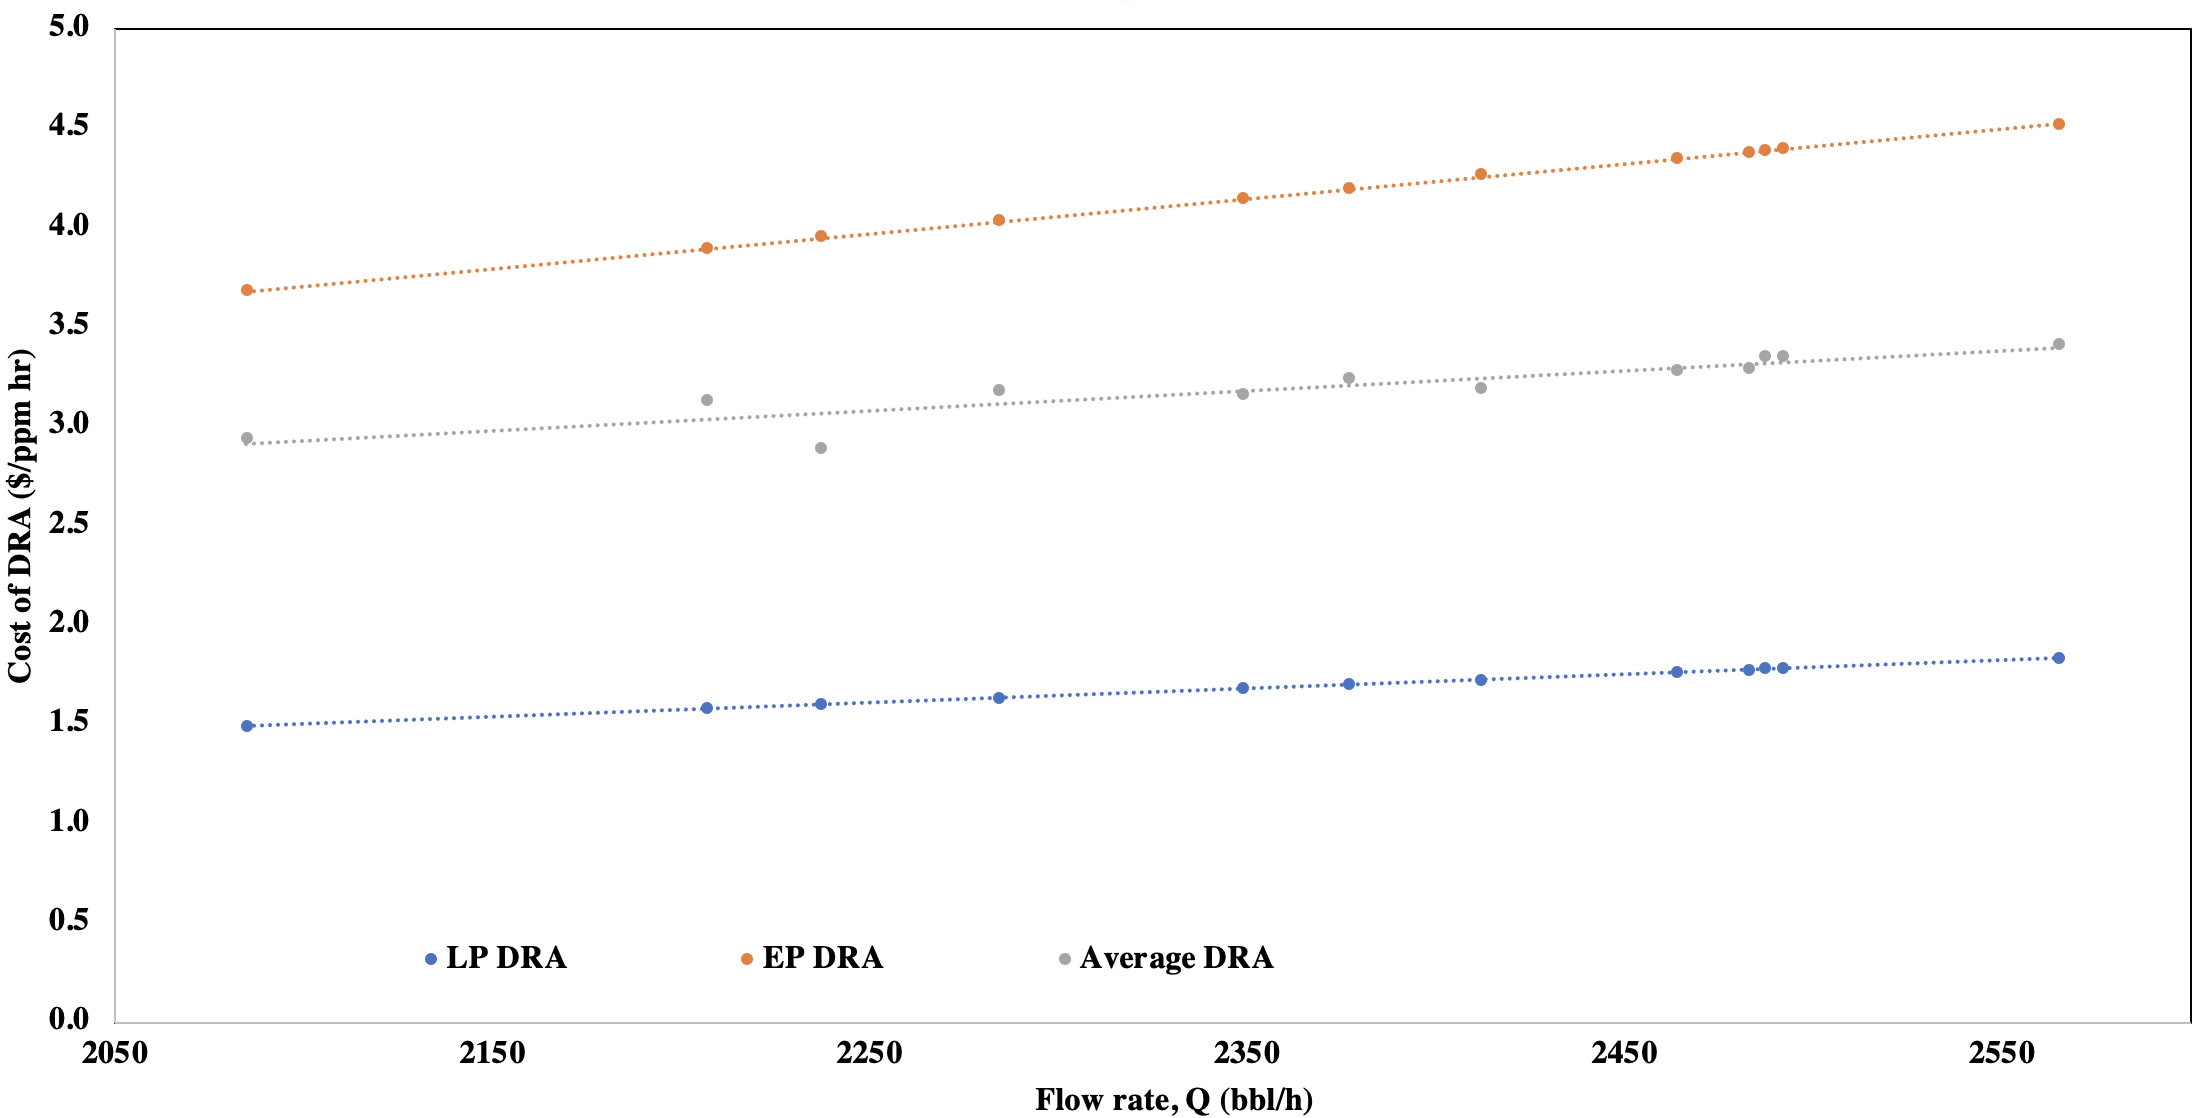
\includegraphics[width=\textwidth]{images/08DRA_Cost.png}
    \caption{Cost of DRA as a function of flow rate.}
    \label{fig:08DRA_Cost}
\end{figure}

\begin{equation}
    \$ / ppm_{sweet} = 0.00071Q + 0.01630
    \label{eq:08sweet_dra}
\end{equation}
\begin{equation}
    \$ / ppm_{sour} = 0.00176Q + 0.00226
    \label{eq:08sour_dra}
\end{equation}
where Q denotes the volumetric flow rate in barrels per hour.

\subsection{Conceptual Software Design}
The conceptual software design for the optimization tool is shown in Figure \ref{fig:08concept_software}. From the right, the users would first populate the costs corresponding to each equipment.  The pump costs are on a \$/kWh basis, and the DRA cost is based on \$/ppm. Operating costs can also be incorporated by multiplying the costs by a fixed factor (e.g. 1.1 $\cdot$ \$/kWh). Currently, DRA costs are calculated automatically based on the historical data using Equations \ref{eq:08sweet_dra} and \ref{eq:08sour_dra}. Next, the user would specify the maximum steady state operating pressure (MSSOP) for the pipeline, and enter the desired flow rate.  Finally, the "OPTIMIZE" button would be pressed and all the boxes outlined in green will be populated with the optimal set point values.  When a set point is no longer deemed optimal, the outline turns red.  An example of such a scenario would be when the batch switches at the CIG or Ault stations.  During maintenance activities, the user can click the "ADVANCED..." button to specify special constraints and eliminate the optimization from using certain equipment. For example, if the Cheyenne VFD is under maintenance, $\nu_{Chey VFD}$ can be constrained to 0, preventing the optimization from using it.

\begin{figure}[h]
    \centering
    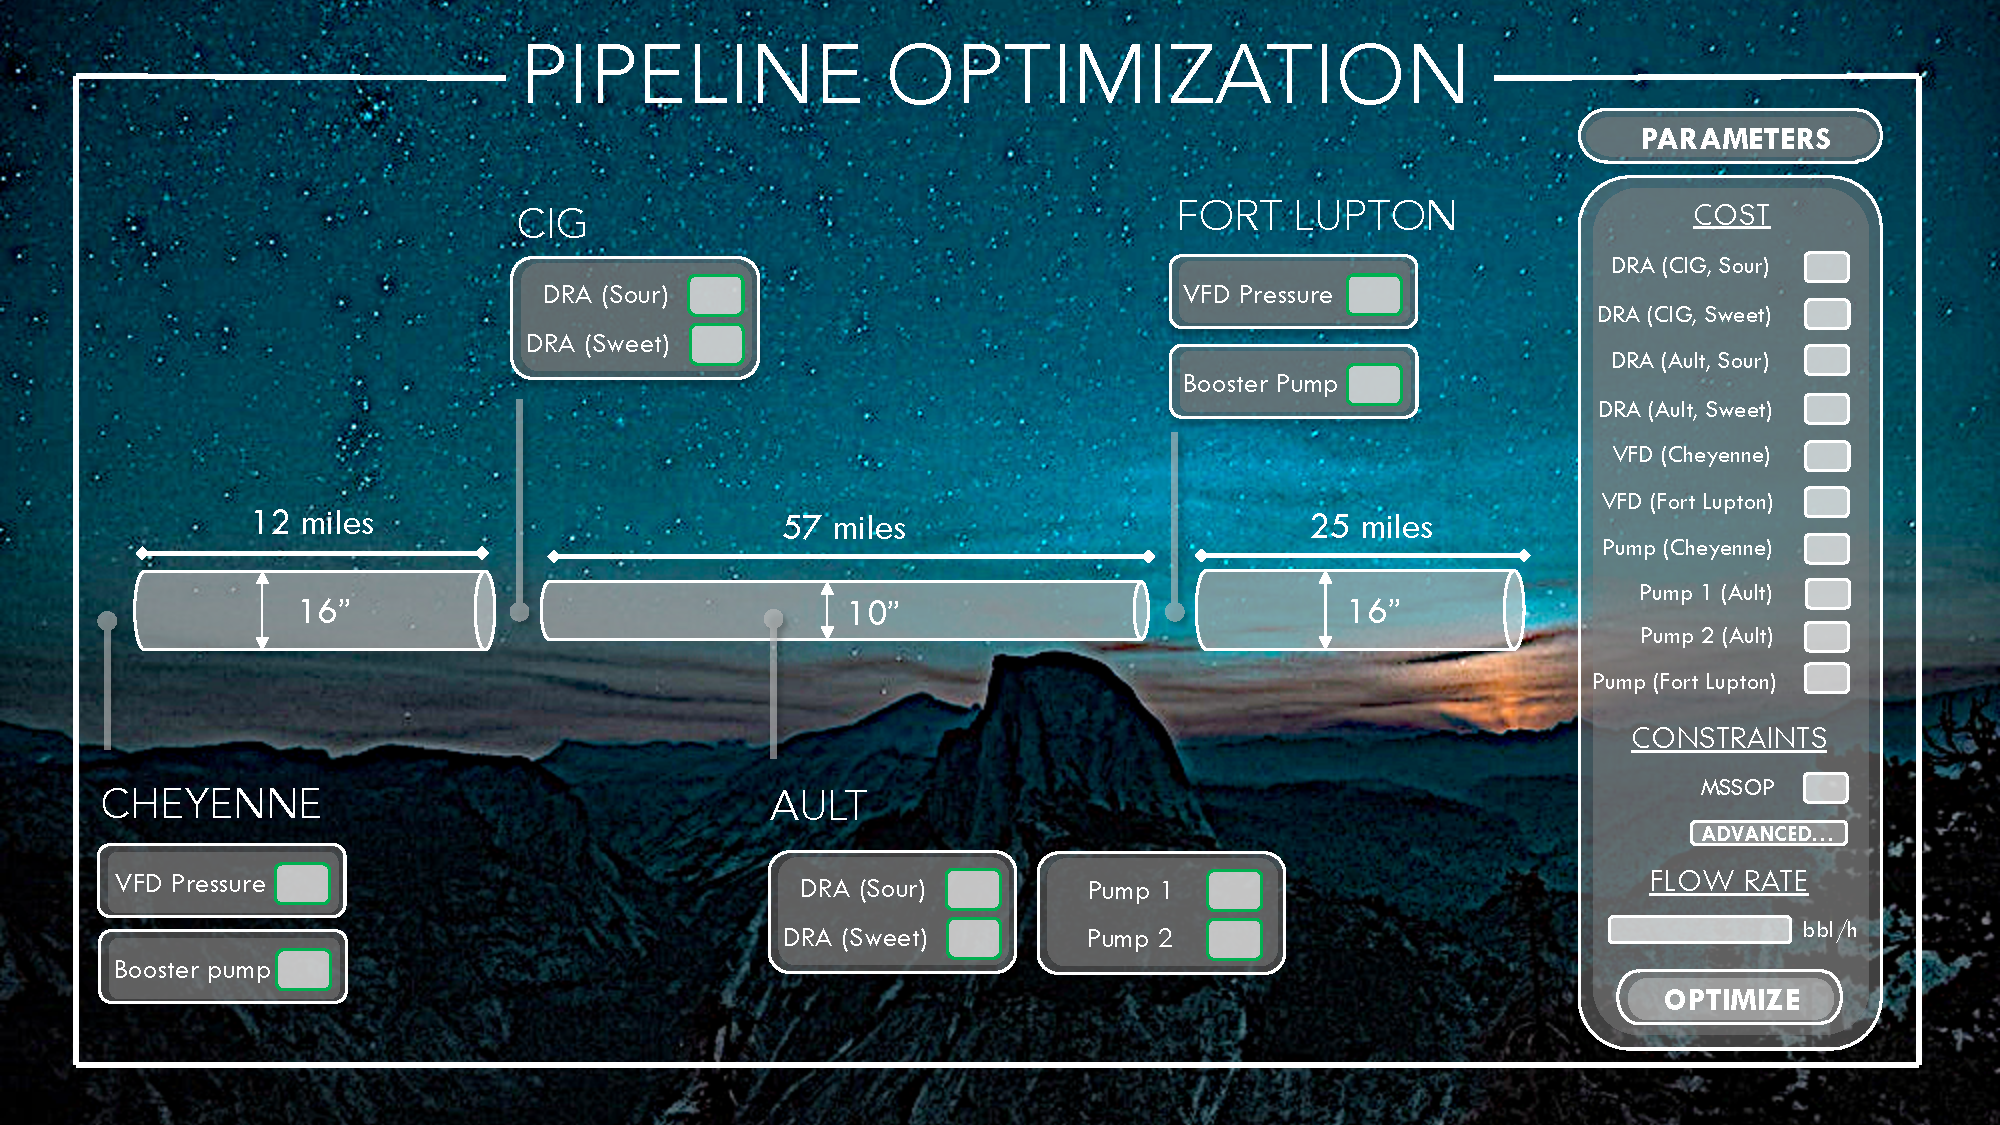
\includegraphics[width=\textwidth]{images/08conceptual_software.pdf}
    \caption{Conceptual software design for the optimization tool.}
    \label{fig:08concept_software}
\end{figure}

A flow diagram of the tool's internal structure is shown in Figure \ref{fig:08Product_Flow}. Starting from the left, the operator would provide the constraints (equipment maintenance, MSSOP, etc.), desired flow rate, and operating costs to the optimization tool.  Likewise, the optimization tool also receives live temperature and density readings from the SCADA system.  Given the densities at CIG and Ault, the proper VFD pumps are turned on.  From the flow rate and DRA pump status, DRA costs are computed from Equations \ref{eq:08sweet_dra} and \ref{eq:08sour_dra}.  Next, the costs, densities, and temperatures are all fed into the machine learning model and the MILP is ran to find the optimal set points to reach the desired flow rate. The set points are then sent to the pressure constraint models to validate that no outlet pressure constraints are violated.  If none are violated, the optimal set points are recommended to the operators. To ensure implementability, the VFD amperes are first converted to pressure set points.

\begin{figure}[h]
    \centering
    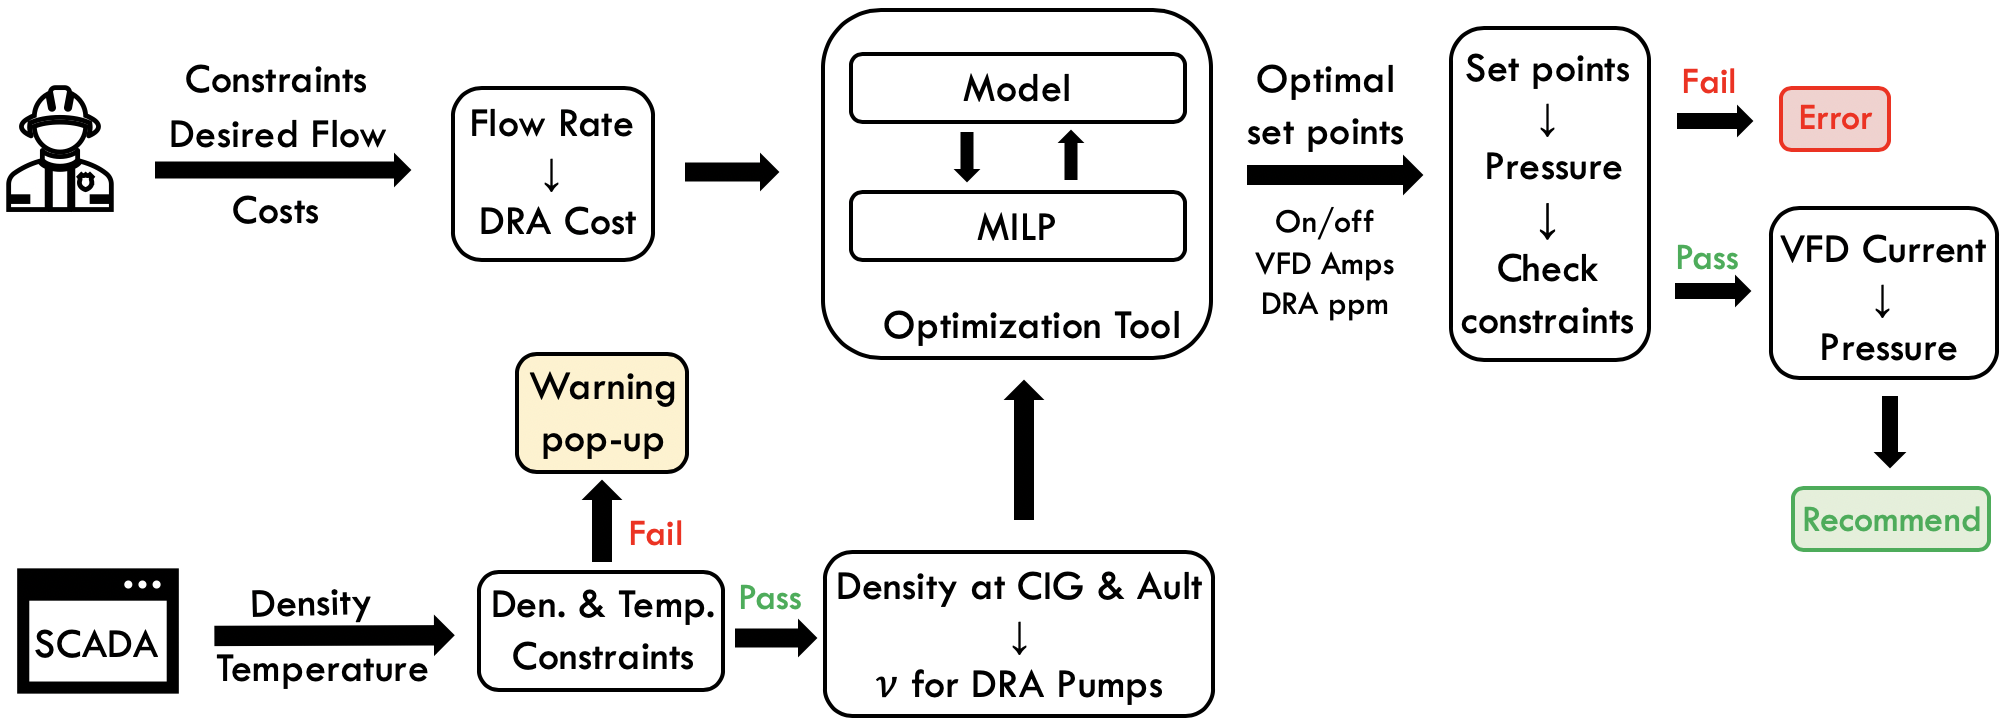
\includegraphics[width=\textwidth]{images/08Product_Flow.png}
    \caption{Internal flow diagram of the product.}
    \label{fig:08Product_Flow}
\end{figure}

\subsection{Cost Savings and Impact on Society}
Operating costs for running the pipeline using the optimization tool was compared to historical values to identify the potential cost savings.  In 2019, the pipeline was plagued with unexpected shut downs and maintenances. Thus, the data set ranging from January 2018 - May 2018 was used for this comparison due to the stability of operations. Both the actual and optimal costs are calculated using the same formulation to ensure a fair comparison.  

First, the total monthly DRA cost was calculated by:
\begin{equation}
    Cost_{DRA} = \sum\limits^{43,200}_{i=1} \frac{1}{60} \left(f_{sweet}(Q, ppm) + f_{sour}(Q, ppm)\right)
    \label{eq:08dra_cost}
\end{equation}
where the functions represent Equations \ref{eq:08sweet_dra} and \ref{eq:08sour_dra} for computing the DRA cost per hour. Here, $i$ denotes the $i^{th}$ minute in a particular month. The costs are divided by 60 to obtain the per minute costs and are summed over 43,200 entries representing the total minutes in a 30 day month. Likewise, the monthly power costs are calculated by:
\begin{equation}
    Cost_{power} = \frac{p}{1000} \sum\limits^{1,800}_{i=1} \sum\limits^{6}_{j=1} I_j \cdot V_j
    \label{eq:08power_cost}
\end{equation}
where $i$ denotes the $i^{th}$ hour in a particular month and $j$ denote the $j^{th}$ pump. $p$ denotes the power cost in kWh. Additionally, $I_j$ and $V_j$ denotes the current and voltage for the $j^{th}$ pump.

The actual and optimal costs for DRA and power are shown in Table \ref{tab:08opt_vs_act_costs}.  It can be seen that the total savings range between -3.7\% - 17.6\%.  The savings were realized by using less DRA while running the pumps harder. For this initial study, interaction effects between pumps and DRA were not explicitly considered. Additionally, the effectiveness of the pumps (i.e., flow rate as a function of current) were assumed to be constant; this may not be the case in actual production because pumps' efficiency changes with accordance to the pump curve \cite{fluid_mechanics}. Likewise, DRA effectiveness was also assumed to be constant; however, preliminary data analysis showed a exponential decay relationship between flow rate and increased DRA.  Additionally, the system was assumed to transition to the desired set point immediately after the set points are inputted for the optimal costs. The average flow rate change between time steps was 8 bbl/h and pressure is propagated down the pipeline at 1480 m/s.  Thus, the error for this assumption is not large. A loss was incurred in April because Suncor used only 10 - 15 ppm of DRA for a large part of the month. In the optimization, minimum DRA was constrained at 20 ppm.

\begin{table}[h]
    \centering
    {\setstretch{1.2}
\begin{tabular}{cc|c|c|c|c|c}
                                                 &            & January & February & March & April & May \\ \hline
\multicolumn{1}{c|}{\multirow{3}{*}{\rotatebox[origin=c]{90}{Actual}}}    & DRA cost   & 102.2 & 114.2 &    106.2 & 84.8 & 140.3 \\
\multicolumn{1}{c|}{}                            & Power cost & 52.3 & 61.6 & 59.7 & 54.0 & 66.5 \\
\multicolumn{1}{c|}{}                            & Total cost & 154.5 & 175.8 & 165.9 & 138.8 & 206.8 \\\hline
\multicolumn{1}{c|}{\multirow{3}{*}{\rotatebox[origin=c]{90}{Optimal}}}     & DRA cost   & 84.9 & 80.6 &    90.9 & 84.9 & 99.7 \\
\multicolumn{1}{c|}{}                            & Power cost & 57.3 & 64.2 & 62.0 & 59.1 & 87.0 \\
\multicolumn{1}{c|}{}                            & Total cost & 142.2 & 144.8 & 152.9 & 144.0 & 186.7 \\ \hline
\multicolumn{1}{c|}{\multirow{2}{*}{\rotatebox[origin=c]{90}{Diff.}}} & Dollars    & \textbf{12.3} & \textbf{31.0} & \textbf{13.0} & \textbf{\textcolor{red}{(5.2)}} & \textbf{20.1} \\
\multicolumn{1}{c|}{}                            & \% change        & \textbf{8.0} & \textbf{17.6} & \textbf{7.8} & \textbf{\textcolor{red}{(3.7)}} & \textbf{9.7}    
\end{tabular}}
    \caption{Optimal vs. actual costs (\$USD 000's) for January - May 2018.}
    \label{tab:08opt_vs_act_costs}
\end{table}

Figures \ref{fig:08Sweet_dra_curve} and \ref{fig:08Sour_dra_curve} shows the flow rate change (normalized by dP) as a function of DRA ppm. The flow rates were normalized by pressure to ensure only the DRA's effect was explored.  The flow rate was normalized by:
\begin{equation}
    Time_{norm} = \frac{Time}{P_2 - P_1}
\end{equation}
where $P_1$ and $P_2$ are the pressures at the starting and ending pump stations, respectively. A similar relationship is expected to exist for pumps due to the pump curves.  To further improve the accuracy of the optimization tool, the weights of the model can be switched to functions.  
\begin{figure}
    \centering
    \begin{subfigure}[b]{0.48\textwidth}
        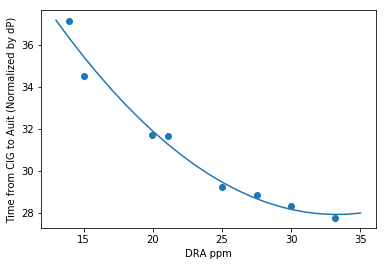
\includegraphics[width=\textwidth]{images/08Sweet_dra_curve.png}
        \caption{Sweet DRA}
        \label{fig:08Sweet_dra_curve}
    \end{subfigure}
    \begin{subfigure}[b]{0.48\textwidth}
        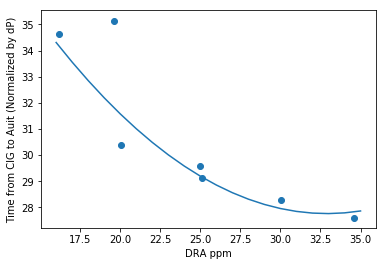
\includegraphics[width=\textwidth]{images/08Sour_dra_curve.png}
        \caption{Sour DRA}
        \label{fig:08Sour_dra_curve}
    \end{subfigure}
        \caption{Flow rate as a function of DRA ppm.}
        \label{fig:my_label}
\end{figure}

A detailed analysis of the cost savings for January - May 2018 are shown in Table \ref{tab:08Cost_per_barrel}. It can be seen that savings per barrel is more significant at higher flow rates.  

\begin{table}[h]
    \centering
    {\setstretch{1.2}
    \begin{tabular}{c|c|c|c|c|c}
                       & January & February & March & April & May  \\ \hline
        Ave. flow rate (bbl/h) & 2195    & 2400     & 2256  & 2248  & 2575 \\
        Saving / bbl per hour (\$)      & 5.6     & 12.9     & 5.7   & \textcolor{red}{(2.3)} & 7.8\\
        Saving / bbl / hour / km (\$) & 0.037 & 0.085 & 0.038 & \textcolor{red}{(0.015)} & 0.052 \\
    \end{tabular}}
    \caption{Cost savings per barrel of crude shipped.}
    \label{tab:08Cost_per_barrel}
\end{table}

Ultimately, expected operating cost savings were estimated to be between 7\% to 9\%.  Average saving per barrel was \$5.95, increasing as the flow rate increased. Moreover, savings for transporting one barrel of crude one km was \$0.04 USD.  The total expected savings per year for Line RM06A was estimated to be \$105,600 USD.  However, the results are only realized if the pipeline is operating within the ranges provided in Tables \ref{tab:08StateConst} and \ref{tab:08InputConst}.

\subsubsection{Benefits for Society}
On the financial side, this optimization tool has shown to reduce operating costs of transporting one bbl/h/km by \$0.04 USD for an industry leading energy company. Cost savings can be even more significant for lower tier, in-experienced companies. In Canada alone, 175,000 barrels of crude is produced per hour and transported at an average velocity of 9.5 km/h \cite{canada_crude_facts}.  Assuming a \$0.04 USD savings per barrel/km results in an annual saving of \$583M USD (\$784M CAD).  Expanding to North America, where approximately 742,000 barrels of crude is produced per hour, the savings jump up to \$2.5B USD (\$3.4B CAD) \cite{NA_crude_facts}. Moreover, the savings here does not include inter-refinery and inter-market pipelines; only produced crude were included.  The savings can be reinvested into greener products, resulting in significant reduction of green house gases (GHG). In 2018, the social cost of carbon was valued at \$46 USD per metric ton \cite{cost_of_carbon}; \$2.5B results in a 54.3M metric ton of reduced GHG.

On the operational level, this tool standardizes operation of complex pipelines. Given a set of inputs, $I = \{Q, Costs, x\}$, the output of the optimization tool each time will be identical due to the linear model. Thus, operators on different shifts and with different experience levels will operate very similarly if this tool is used.  Additionally, this normalization reduces variance in operations which reduces depreciation of process equipment. Furthermore, the free cash flow can be reinvested to obtain higher throughputs, which in turn will increase revenue and increase tax dollars.  Finally, the tool will also increase operational safety, which may result in the Alberta Energy Regulator (AER) allowing higher throughputs on pipelines currently operating under capacity.
